%%%%%%%%%%%%%%%%%%%%%%%%%%%%%%%%%%%%%%%%%%%%%%%%%%%%%%%%%%%%%%%%%%%%%%%%%%%%%%%%
%%%%%%%%%%%%%%%%%%%%%%%%%%%%%%%%%%%%%%%%%%%%%%%%%%%%%%%%%%%%%%%%%%%%%%%%%%%%%%%%
\part{Category Theory}\label{part:category_theory}
\cite{awodey06}\cite{maclane69}
%%%%%%%%%%%%%%%%%%%%%%%%%%%%%%%%%%%%%%%%%%%%%%%%%%%%%%%%%%%%%%%%%%%%%%%%%%%%%%%%
%%%%%%%%%%%%%%%%%%%%%%%%%%%%%%%%%%%%%%%%%%%%%%%%%%%%%%%%%%%%%%%%%%%%%%%%%%%%%%%%

Membership (\S\ref{sec:membership}) as the Fundamental Primitive of
Set Theory (Part \ref{part:set_theory})

Composition (\S\ref{sec:composition}) as the Fundamental Primitive of
Category Theory

2016Leinster - \emph{Basic Category Theory}

2018Hopkins - \emph{All of Basic Category Theory} (slides)



% ==============================================================================
\section{Metacategory}\label{sec:metacategory}
% ==============================================================================

The Formal System of Category Theory consists of:
\begin{itemize}
\item two Sorts (\S\ref{sec:sort}), \emph{Objects} $A,B,C,\ldots$, and
  \emph{Arrows} (corresponding to Morphisms) $f,g,h,\ldots$
\item four Operations: $dom(f)$, $cod(f)$, $1_A$, $\circ$
\end{itemize}
and seven Axioms:
\[
  dom(1_A) = A,\quad cod(1_A) = A
\]\[
  f \circ 1_{dom(f)} = f, \quad 1_{cod(f)} \circ f = f
\]\[
  dom(g\circ f) = dom(f), \quad cod(g \circ f) = cod(g)
\]\[
  h \circ (g \circ f) = (h \circ g) \circ f
\]

Composition (\S\ref{sec:composition})

Subsumption Relation (\S\ref{sec:subsumption_relation})



% ------------------------------------------------------------------------------
\subsection{Abstract Category}\label{sec:abstract_category}
% ------------------------------------------------------------------------------

The \emph{Elementary Theory of Abstract Categories} refers to the
First-order Formulas (\S\ref{sec:predicate_logic}) of the Language
of Metacategories.

A Sentence, $\Sigma$, in the Elementary Theory of Abstract Categories
can be made into a Dual Sentence, $\Sigma^*$, by replacing instances
of $cod$ by $dom$ and $dom$ by $cod$, and $h = g \circ f$ with $h = f
\circ g$. The Double-dual is Idempotent (\S\ref{sec:idempotent}):
$\Sigma^{**} = \Sigma$.

Because the Axioms are Self-dual, if a Sentence can be derived from
them, so can its Dual by the Duality Principle
(\S\ref{sec:duality_principle}). Functors (\S\ref{sec:functor}) are
Self-dual, and so they are not reversed as are Morphisms in
Categories.



% ------------------------------------------------------------------------------
\subsection{Paracategory}\label{sec:paracategory}
% ------------------------------------------------------------------------------

Quiver (\S\ref{sec:quiver})



% ------------------------------------------------------------------------------
\subsection{Precategory}\label{sec:precategory}
% ------------------------------------------------------------------------------

A \emph{Precategory} (or \emph{Diagram Scheme}), $G$, is a Directed Graph
(\S\ref{sec:directed_graph}) in the context of Category Theory. A Precategory is
used to generate a \emph{Free Category} (\S\ref{sec:free_category}). Here we
will use the notation for Categories (\S\ref{sec:category}) to equate Vertices
with Objects $G_0$ and Edges with Morphisms $G_1$. A Precategory can then be
described as a pair of Functions, $cod$ and $dom$, from the Set of Edges to the
Set of Objects:
\[
  G = \{G_1 \rightrightarrows G_0\}
\]

A Morphism $D : G \rightarrow G'$ between Precategories is a pair of Functions:
\[
  D_0 : G_0 \rightarrow G'_0, \;\;\; D_1 : G_1 \rightarrow G'_1
\]
such that $\forall f \in G_1$:
\[
  D_0(dom(f)) = dom(D_1(f))
\]\[
  D_0(cod(f)) = cod(D_1(f))
\]
Given two Graphs, $A$ and $B$, with the same Set of Objects, $O$, the Product
$\times_O$ over $O$ is defined as:
\[
  A \times_O B = \{ (g,f) | dom(g) = cod(f), g \in A, f \in B \}
\]
the set of Composable Morphisms.

A Category can be seen as a Graph, $G$, with two Morphisms:
\begin{enumerate}
  \item Mapping Composable Morphisms to their Composite:
    \[c : G \times_{G_0} G \rightarrow G\]
  \item Mapping Objects to their Identity Functions:
    \[i: G_0 \rightarrow G_1\]
\end{enumerate}
The \emph{Underlying Graph} of a Category, $\cat{C}$, is denoted
$U(\cat{C})$ where $U$ is the \emph{Underlying Graph Functor}
(\S\ref{sec:functor}).

For a Morphism of Graphs, $D : G \rightarrow U(\cat{B})$, there is
a corresponding Functor of Categories: $D' : \cat{C}_G \rightarrow
\cat{B}$.

The Category of all Small Directed Graphs and Graph Morphisms is
$\cat{Grph}$.

The Forgetful Functor (\S\ref{sec:forgetful_functor}) $U : \cat{Cat}
\rightarrow \cat{Grph}$ Maps a Categories to their Underlying Graphs,
effectively forgetting which Morphisms are Identities and which are
Composites.



% ------------------------------------------------------------------------------
\subsection{Free Category}\label{sec:free_category}
% ------------------------------------------------------------------------------

A \emph{Free Category} (or \emph{Path Category}) $F(G)$ (or
$\cat{C}_G$) is Generated (\S\ref{sec:generator}) by a Directed Graph
or Precategory (\S\ref{sec:precategory}), $G$, of Vertices and Arrows
under Concatenation of Paths.

For a Graph with a single Vertex, the Free Category is the Free Monoid
on the Edges of the Graph. A Graph with no Edges generates a Discrete
Category (\S\ref{sec:discrete_category}). The Free Category on a Graph
with two Vertices and one Edge between them is the Finite Category
(\S\ref{sec:finite_category}) $\cat{2}$. The Category $\cat{2}$ is a
Generator for the Category of all Categories.

Any Directed Acyclic Graph generates a Partial Order as its Free
Category.



% ------------------------------------------------------------------------------
\subsection{Category Presentation}\label{sec:category_presentation}
% ------------------------------------------------------------------------------

Presentation (\S\ref{sec:presentation})

Generators (\S\ref{sec:generator}): Directed Graph $G = (V,A)$

Free Category (\S\ref{sec:free_category}) $F(G)$

Relation: $R : F(G) \times F(G) \rightarrow R_{-,-} \subseteq
F(G)(-,-)$ ??? %FIXME

Quotient Category (\S\ref{sec:quotient_category}) $F(G) / R$

generalization of $T$-algebra Presentation
(\S\ref{sec:t_algebra_presentation})

``a Category with \emph{Weak Equivalences} (\S\ref{sec:weak_equivalence}) is
just a \emph{Presentation} of an $\infty$-category (or a Homotopy Theory)``

--\url{https://golem.ph.utexas.edu/category/2017/11/internal_languages_of_higher_c_1.html}



% ------------------------------------------------------------------------------
\subsection{Vertical Categorification}
\label{sec:vertical_categorification}
% ------------------------------------------------------------------------------

% ------------------------------------------------------------------------------
\subsection{Horizontal Categorification}
\label{sec:horizontal_categorification}
% ------------------------------------------------------------------------------

Monads (\S\ref{sec:monad}) are a Horizontal Categorification of
Monoids



% ==============================================================================
\section{Category}\label{sec:category}
% ==============================================================================

A \emph{Category} is an Algebraic Structure (\S\ref{sec:algebraic_structure})
where Functions are Morphisms (\S\ref{sec:morphism}) between Objects and each
Object has a Unique \emph{Identity Morphism} and where Composition of Morphisms
is Associative and Transitive.

A Category $\cat{C}$ is defined as:
\begin{itemize}
\item a Class $C_0$ of Objects (\S\ref{sec:category_object})
\item a Class $C_1$ of Morphisms (\S\ref{sec:morphism}; also called
  \emph{Arrows} or \emph{Maps}) with Identity Morphisms for each Object
\item a Binary Associative and Transitive Composition Operation on Morphisms
\end{itemize}
$\cat{C}$ is considered \emph{Small} (as opposed to \emph{Large})
if both $C_0$ and $C_1$ can be represented as Sets.

An equivalent definition of Categories can be given in terms of
\emph{Hom-sets} (\S\ref{sec:hom_set}).

a Category can be seen as a Monoid (\S\ref{sec:monoid}) with \emph{Type
  Parameters}, i.e. a Monoid is a Category with only one Object

(Corfield2018): Partially Ordered Sets (\S\ref{sec:poset}) can be considered as
Categories ``enriched'' in Truth Values (\S\ref{sec:truth_value}) (FIXME:
clarify)

\url{https://golem.ph.utexas.edu/category/2018/02/gradual_typing.html}:

Dynamic Types (\S\ref{sec:dynamic_typing}) are to Typed Languages as
\emph{Monoids} are to \emph{Categories}, or \emph{Operads} to
\emph{Multicategories}

\asterism

Example Categories:
\begin{itemize}
\item Sets and (Set) Functions
\item Finite Sets and Injective Functions
\item Posets and Monotonic Functions
\item Monoids and Monoid Homomorphisms
\item Groups and Group Homomorphisms
\item Categories and Functors
\item Formulae and Deductions
\item Functors and Natural Transformations
\item Types and Computable Functions
\end{itemize}
The Category of all Sets and Set Mappings is denoted $\cat{Set}$
(and is Dual to the Category of Complete, Atomic Boolean Algebras
(\S\ref{sec:boolean_algebra}). See \emph{List of Categories}
\S\ref{sec:categories_list} for more examples of Categories.

any Category with at most one Morphism between any two Objects is a Preorder:
(\S\ref{sec:preorder}): Preorders represent Categories by taking Elements as
Objects and (Single) Morphisms existing between Pairs of Elements in the
Ordering Relation which satisfies the Category Axioms by the Reflexivity and
Transitivity of the Preorder.

The Category of Posets is denoted $\cat{Pos}$. A special case of a
Poset Category is a Discrete Category (\S\ref{sec:discrete_category})
which is a Category of Objects with only Identity Morphisms.

A Monoid (\S\ref{sec:monoid}) is a Category with a single Object and
Morphisms for each Element in the Monoid such that Composition of
Morphisms is the Binary Operation of the Monoid. The Category
$\cat{Mon}$ is the Category of all Monoids and Functions that
preserve the Monoid structure.

Simplex Category (\S\ref{sec:simplex_category})



% ------------------------------------------------------------------------------
\subsection{List of Categories}\label{sec:categories_list}
% ------------------------------------------------------------------------------

\begin{description}
\item [0] no Objects or Morphisms
\item [1] one Object with Identity Morphism
\item [2] two Objects with Identity Morphisms and one Morphism between
  them
\item [3] three Objects with Identity Morphisms in a Commutative
  Triangle
\item [$\downdownarrows$] two Objects and two Parallel Morphisms
  between them
\item [$\omega$] the ordinals $\omega$ as a Poset
\item [Set] all Small Sets and Functions (Locally Small)
\item [Set$^\omega$] Sets through time: Functors from $cat{\omega}$
  to $\cat{Set}$ as Objects and Natural Transformations between
  them as Morphisms
\item [Set$^\downdownarrows$] Graph and Graph Homomorphisms
\item [Cls] all Classes and Functions between Classes
\item [Set$_*$] all Pointed Sets and Base-point preserving Functions
\item [Par] all Sets and Partial Functions
\item [Rel] all Sets and Relations
\item [Pos] all Posets and Monotonic Functions (Locally Small)
\item [Cpo] all Complete Partial Orders and Continuous Functions
  (Domain Theory \S\ref{sec:domain_theory})
\item [$\omega$Cpo] all $\omega$-cpos and Continuous Functions
\item [FinSet] all Finite Sets and Functions (Full Subcategory of
  $\cat{Set}$)
\item [FinOrd] ($\cat{\Delta}$) all Finite Ordinal Numbers and
  Order Preserving Maps (Skeleton of $\cat{FinSet}$, also called
  the \emph{Simplex Category} \S\ref{sec:simplex_category})
\item [Mag] all Magmas and Homomorphisms of Operations
\item [Med] all Medial Magmas and Homomorphisms of Operations
\item [Mon] all Monoids and Monoid Homomorphisms
\item [Grp] all Groups and Group Homomorphisms (Locally Small)
\item [Ab] all Abelian Groups with Group Homomorphisms
\item [Grpd] all Groupoids and Groupoid Homomorphisms
\item [Rng] all Small Rings and Ring Morphisms
\item [CRing] all Commutative Rings and Ring Homomorphisms
\item [RCR] all Real Closed Rings and Ring Homomorphisms
\item [Aff] all Affine Schemes (\S\ref{sec:affine_scheme}) and Homorphisms of
  Affine Schemes
\item [$R$-Mod] all $R$-modules (\S\ref{sec:module})
\item [Grph] all Small Graphs and Graph Morphisms; the Category of Graphs and
  Graph Homomorphisms is also an example of a Topos (\S\ref{sec:topos})
\item [Quiv] all Quivers and Quiver Morphisms
\item [Cat] all Small Categories and Functors (2-category
  \S\ref{sec:2_category})
\item [Cat'] all Large Categories and Functors
\item [StrCat] all Strict Categories (\S\ref{sec:strict_category}) and
  Functors
\item [Prof] all Small Categories and Profunctors
  (\S\ref{sec:profunctor}) with Natural Transformations between them
\item [DagCat] all Dagger Categories (\S\ref{sec:dagger_category}) and
  Dagger Functors (\S\ref{sec:dagger_functor})
\item [Top] all Topological Spaces and Continuous Maps (Locally Small)
\item [Top$_*$] all Pointed Topological Spaces and Continuous Maps
\item [CGTop] all Compactly Generated Spaces
  (\S\ref{sec:compactly_generated}) and (???) Continuous Maps (Full
  Subcategory of $\cat{Top}$)
\item [CGHaus] all Hausdorff Spaces (\S\ref{sec:hausdorff_space}) and
  (???) Continuous Maps (Full Subcategory of $\cat{CGTop}$)
\item [Toph] all Topological Spaces and Homotopy Classes of Continuous
  Maps (Homotopy Category \S\ref{sec:homotopy_category}, not
  Concretizable \S\ref{sec:concrete_category})
\item [Hotc] all CW Complexes and Homotopy Classes of Continuous Maps
\item [Man] or $\cat{Diff}$ all Smooth Manifolds (\S\ref{sec:smooth_manifold})
  and Smooth Maps; Differentiation (\S\ref{sec:derivative}) may be defined as an
  Endofunctor $\mathrm{d} : \cat{Diff} \rightarrow \cat{Diff}$ sending Smooth
  Manifolds $X$ to \emph{Tangent Bundles} (\S\ref{sec:tangent_bundle}) $T X$,
  with Points of $T X$ being Ordered Pairs $(x, v)$ where $v$ is a \emph{Tangent
    Vector} at $x$
\item [Cob] all Closed Manifolds and Cobordisms
\item [Euc] Euclidean Spaces $\reals^n$ and Smooth Maps
\item [Vect$_K$] all Finite-dimensional Vector Spaces over Field $K$
  and $K$-linear Transformations
\item [Vect$_\reals$] all Finite-dimensional Vector Spaces over
  $\reals$ and Linear Maps
\item [LinRel] all Vector Spaces and Linear Relations %FIXME
\item [LagRel$_k$] PROP Category (\S\ref{sec:prop_category}) of Symplectic
  Vector Spaces (\S\ref{sec:symplectic_vectorspace}) of the form $k^{2n}$ and
  Linear Lagrangian Relations as Morphisms
\item [Hilb] all Hilbert Spaces (\S\ref{sec:hilbert_space}) and Short
  Linear Maps (\S\ref{sec:short_linear}); is a Dagger Compact Category
  (\S\ref{sec:dagger_compact})
\item [FdHilb] all Finite-dimensional Hilbert Spaces and Short Linear
  Maps (???)
\item [Prob] all Probability Spaces and ``Almost-everywhere-equality Equivalence
  Classes'' of Measure-preserving Maps
\item [Loc] all Locales and Maps of Locales (Meet preserving Functions
  with Left Adjoints preserving Finite Meets)
\item [Frm] all Frames and Monotone Functions preserving Finite Meets
  and arbitrary Joins
\item [CHey] all Complete Heyting Algebras and their Homomorphisms
\item [BA] all Boolean Algebras and their Homomorphisms
\item [Law] all Lawvere Theories (\S\ref{sec:lawvere_theory}) and Maps
  of Lawvere Theories
\item [C($\lambda$)] all Types and Closed Terms
\end{description}

Database Schema (\S\ref{sec:database_schema}): Tables and Foreign Keys

$\cat{Set}$ -- Locally Cartesian Closed
(\S\ref{sec:locally_cartesian_closed})

Higher Categories:

%FIXME some of the above listed may in fact be ``higher'' categories

\begin{itemize}
\item [$\infty$Grpd] the $(\infty,1)$-category of $\infty$-groupoids
  (\S\ref{sec:infinity_groupoid}), i.e. of $(\infty,0)-categories$
\item ... TODO
\end{itemize}



% ------------------------------------------------------------------------------
\subsection{Composition}\label{sec:composition}
% ------------------------------------------------------------------------------

2017 - Hedges - \emph{On compositionality} -
\url{https://julesh.com/2017/04/22/on-compositionality/} -- ``the opposite of
Compositionality is \emph{Emergent Effects}''

\url{http://lambda-the-ultimate.org/node/5550}



\subsubsection{Transfinite Composition}
\label{sec:transfinite_composition}

Composition of Infinitely many Morphisms



% ------------------------------------------------------------------------------
\subsection{Hom-set}\label{sec:hom_set}
% ------------------------------------------------------------------------------

The collection of all Morphisms between two Objects $X$ and $Y$ in a
Category $\cat{C}$ is called the \emph{Hom-set} and is denoted
$Hom(X,Y)$:
\[
  Hom(X,Y) = \{f \in \cat{C} | f : X \rightarrow Y\}
\]
This gives a Hom-functor (\S\ref{sec:hom_functor}):
\[
  Hom_\cat{C} : \cat{C^{op}} \times \cat{C} \rightarrow \cat{Set}
\]
each half of which is a Representable Functor
(\S\ref{sec:representable_functor}).
\newline
\fist Note that the Hom-set need not be a Set (it could be a
Proper Class). A Category for which all Hom-sets are Sets is called a
Locally Small Category (\S\ref{sec:locally_small}).

Some Properties of Hom-sets:
\begin{itemize}
\item $ (X,Y) \neq (X',Y') \Rightarrow
  Hom(X,Y) \cap Hom(X',Y') = \varnothing$
\end{itemize}

A definition of Categories can be given in terms of Hom-sets. %FIXME

Internal Hom-set

External Hom-set



% ------------------------------------------------------------------------------
\subsection{Finite Category}\label{sec:finite_category}
% ------------------------------------------------------------------------------

A \emph{Finite Category} has a Finite number of Morphisms and Objects.
An Infinite number of Objects implies an Infinite number of Morphisms
because each Object has its own Identity Morphism.

A Category such as:
\[
  A
  \begin{matrix}
  \xrightarrow{\;\;f\;\;}\\
  \xleftarrow[\;\;g\;\;]{}
  \end{matrix}
  B
\]
induces an Infinite Category if $f$ and $g$ are not Isomorphisms
(\S\ref{sec:isomorphism}) because new Morphisms exist wherever the
Codomain of one Morphism is the Domain of another: $gf, gfgf, gfgfgf,
\ldots$ and $fg, fgfg, fgfgfg, \ldots$. See \emph{Finitely Presented
  Categories} (\S\ref{sec:finitely_presented}).

\begin{itemize}
  \item $\cat{0}$: Empty Category (\S\ref{sec:empty_category})
    \[
      \varnothing
    \]

    Initial Object in $\cat{Cat}$, Empty Groupoid
    (\S\ref{sec:groupoid}), Empty Set

  \item $\cat{1}$
    \[
      \bullet
    \]

    Terminal Object in $\cat{Cat}$

  \item $\cat{2}$
    \[
      \bullet \longrightarrow \circ
    \]

    Properties:
    \begin{enumerate}
    \item Generator for $\cat{Cat}$ %FIXME xref generator
    \item Retract of every Generator
    \end{enumerate}

    Endofunctors: $1_\cat{2}$, $\Delta_\bullet$, $\Delta_\circ$

\end{itemize}

Functors from $\cat{1}$ to $\cat{2}$:
\begin{enumerate}
  \item $\bullet : \cat{1} \rightarrow \cat{2}$
  \item $\circ : \cat{1} \rightarrow \cat{2}$
\end{enumerate}



\subsubsection{Empty Category}\label{sec:empty_category}

\subsubsection{Locally Finite Category}
\label{sec:locally_finite_category}



% ------------------------------------------------------------------------------
\subsection{Small Category}\label{sec:small_category}
% ------------------------------------------------------------------------------

% ------------------------------------------------------------------------------
\subsection{Large Category}\label{sec:large_category}
% ------------------------------------------------------------------------------

% ------------------------------------------------------------------------------
\subsection{Locally Presentable Category}\label{sec:locally_presentable}
% ------------------------------------------------------------------------------



\subsubsection{Locally Finitely Presentable Category}
\label{sec:lfp_category}

\fist Finitely Presented Category (\S\ref{sec:finitely_presented})

\url{https://golem.ph.utexas.edu/category/2017/04/gluing_together_finite_shapes.html}



% ------------------------------------------------------------------------------
\subsection{Accessible Category}\label{sec:accessible_category}
% ------------------------------------------------------------------------------

Accessible Functor (\S\ref{sec:accessible_functor})



% ------------------------------------------------------------------------------
\subsection{Category Equivalence}\label{sec:category_equivalence}
% ------------------------------------------------------------------------------

An \emph{Equivalence} between two Categories, $\cat{C}$ and
$\cat{D}$, $\cat{C} \simeq \cat{D}$, can be established by a
Pair of Functors (\S\ref{sec:functor}):
\[
  S : \cat{C} \rightarrow \cat{D}
\]\[
  T : \cat{D} \rightarrow \cat{C}
\]
and Natural Isomorphisms (\S\ref{sec:natural_isomorphism}):
\[
  I_\cat{C} \cong T \circ S
\]\[
  I_\cat{D} \cong S \circ T
\]
$S$ and $T$ in such an Equivalence are Fully Faithful
(\S\ref{sec:fully_faithful}).

\fist Note Equality of Categories $\simeq$ is distinct from
Isomorphism of Categories $\cong$.

$\cat{Set}_{fin} \simeq \cat{Ord}_fin$

$\cat{Par} \cong \cat{Set}$

$\cat{Set}^I \simeq \cat{Set}/I$

$\cat{BA}_{fin} \simeq \cat{Set}_{fin}^{op}$

$\cat{caBA} \simeq \cat{Set}^{op}$ Complete Atomic Boolean
Algebras %FIXME xref



% ------------------------------------------------------------------------------
\subsection{Subcategory}\label{sec:subcategory}
% ------------------------------------------------------------------------------

A \emph{Subcategory}, $\cat{S}$, of a Category, $\cat{C}$, is a
Category whose Objects and Morphisms are in $\cat{C}$.

For a Monomorphism in $\cat{Cat}$ from a Category $\cat{E}$ such
that $E$ is an Equalizer:
\[
  \cat{E} \xrightarrow{\;\;E\;\;} \cat{C}
  \begin{matrix}
  \xrightarrow{\;\;F\;\;}\\
  \xrightarrow[\;\;G\;\;]{}
  \end{matrix}
  \cat{D}
\]
$\cat{E}$ is a Subcategory of $\cat{C}$.



\subsubsection{Inclusion Functor}\label{sec:inclusion_functor}

For a Subcategory $\cat{S}$ of a Category $\cat{C}$ there is a
Monomorphic Faithful Functor (\S\ref{sec:faithful_functor}) called the
\emph{Inclusion Functor} which Maps Objects and Morphisms to
themselves:
\[
  I : \cat{S} \rightarrow \cat{C}
\]
If $I$ is a Full Functor then $\cat{S}$ is a \emph{Full
  Subcategory} (\S\ref{sec:full_subcategory}).



\subsubsection{Full Subcategory}\label{sec:full_subcategory}

A Subcategory $\cat{S}$ of a Category $\cat{C}$ is a \emph{Full
  Subcategory}, denoted $\cat{S} \rightarrowtail \cat{C}$ if the
corresponding Inclusion Functor is a Full Functor. A Full Subcategory
consists of some Objects and all Morphisms between them.

The Inclusion Functor $\cat{Set}_{fin} \rightarrowtail
\cat{Set}$ is Fully Faithful (\S\ref{sec:fully_faithful}).



\paragraph{Reflective Subcategory}\label{sec:reflective_subcategory}\hfill

Homoiconicity (\S\ref{sec:homoiconicity})

\emph{Reflector} (\S\ref{sec:reflector})

Coreflective Subcategory

Bireflective



\subparagraph{Reflector}\label{sec:reflector}\hfill


A \emph{Reflector}, $T$, is a Left Adjoint to the Inclusion Functor of
a Full Subcategory $i : \cat{C} \hookrightarrow \cat{D}$:
\[
  (T \dashv i) :
  \cat{C} \stackrel{\xleftarrow{T}}{\hookrightarrow} \cat{D}
\]

Reflection (Homoiconicity \S\ref{sec:homoiconicity})



% ------------------------------------------------------------------------------
\subsection{Discrete Category}\label{sec:discrete_category}
% ------------------------------------------------------------------------------

A Category is \emph{Discrete} if it is Equivalent
(\S\ref{sec:category_equivalence}) or (sometimes) Isomorphic to a
Category with only Identity Morphisms and no others.

The Discrete Category Functor $S : \cat{Set} \rightarrow
\cat{Cat}$ is Fully Faithful (\S\ref{sec:fully_faithful}).



% ------------------------------------------------------------------------------
\subsection{Thin Category}\label{sec:thin_category}
% ------------------------------------------------------------------------------

A \emph{Thin Category} has at most one Morphism between Objects, e.g.
a Preorder (a Poset without Antisymmetry \S\ref{sec:preorder}).

a Skeletal Thin Category is a Poset (\S\ref{sec:poset})



% ------------------------------------------------------------------------------
\subsection{Skeletal Category}\label{sec:skeletal_category}
% ------------------------------------------------------------------------------

A Category is \emph{Skeletal} if Isomorphic Objects are the same
Object. Any Category can be made Skeletal by taking Objects as
Isomorphism Classes of the original Objects.

a Skeletal Thin Category is a Poset (\S\ref{sec:poset})



% ------------------------------------------------------------------------------
\subsection{Weak Category}\label{sec:weak_category}
% ------------------------------------------------------------------------------

% ------------------------------------------------------------------------------
\subsection{Strict Category}\label{sec:strict_category}
% ------------------------------------------------------------------------------

$\cat{StrCat}$

Category of $T$-algebras (\S\ref{sec:t_algebra}) for a Monad on the
Category of Quivers $\cat{Quiv}$



% ------------------------------------------------------------------------------
\subsection{Localization}\label{sec:category_localization}
% ------------------------------------------------------------------------------

for a Collection $W$ of Morphisms, result of making all Morphisms in
$W$ into Isomorphisms

%FIXME



% ==============================================================================
\section{Morphism}\label{sec:morphism}
% ==============================================================================

% ------------------------------------------------------------------------------
\subsection{Identity}\label{sec:identity_morphism}
% ------------------------------------------------------------------------------

Objects (\S\ref{sec:category_object})



% ------------------------------------------------------------------------------
\subsection{Parallel Morphism}\label{sec:parallel_morphism}
% ------------------------------------------------------------------------------

$f,g : X \rightarrow Y$

Limit: Equalizer (\S\ref{sec:equalizer})

Colimit: Coequalizer (\S\ref{sec:coequalizer})



% ------------------------------------------------------------------------------
\subsection{Monomorphism}\label{sec:monomorphism}
% ------------------------------------------------------------------------------

A \emph{Monomorphism} $f$ between Objects $A$ and $B$ is denoted:
\[
  f : A \rightarrowtail B
\]
and has the property for any two Morphisms $g, h : C \rightarrow A$,
$fg = fh$ Implies $g = h$ ($f$ is Left Cancellative
\S\ref{sec:cancellative_property}). An Monomorphism in a Category
$\cat{C}$ is an Epimorphism in $\cat{C^{op}}$.

If $f$ is a Monomorphism then $gf$ and $hf$ are Idempotent
(\S\ref{sec:idempotent}). %FIXME correct ???

Functions between Sets (any Morphism in a Concrete Category
\S\ref{sec:concrete_category}) are Monomorphisms if they are Injective
Functions. In $\cat{Set}$ Monomorphisms are exactly the Injective
Functions between Sets. This is also true in the Categories
$\cat{Grp}$, $\cat{Rng}$, and any Abelian Category
(\S\ref{sec:abelian_category}).

Equalizers (\S\ref{sec:equalizer}) are always Monomorphisms and as
such are used to define the notion of Subobject
(\S\ref{sec:subobject}).

\fist Note not all Monomorphisms are required to be Injective.

Left-invertible Morphisms are necessarily Monomorphisms (Split
Monomorphism \S\ref{sec:split_monomorphism}).

As a representing Subobjects (\S\ref{sec:subobject}) Monomorphisms in:
\begin{itemize}
  \item $\cat{Set}$ are generalized Subsets
  \item $\cat{Grp}$ are generalized Subgroups
  \item $\cat{Top}$ are generalized Subspaces
\end{itemize}



\subsubsection{Split Monomorphism}\label{sec:split_monomorphism}

A Morphism with a Left Inverse or \emph{Retraction} is a Monomorphism
called a \emph{Split Monomorphism}.

The Retraction of a Split Monomorphism is a Split Epimorphism
(\S\ref{sec:split_epimorphism}).

assuming the Axiom of Choice, all Monomorphisms in $\cat{Set}$ are
Split



\subsubsection{Regular Monomorphism}\label{sec:regular_monomorphism}

\subsubsection{Strong Monomorphism}\label{sec:strong_monomorphism}

\subsubsection{Extremal Monomorphism}\label{sec:extremal_monomorphism}



% ------------------------------------------------------------------------------
\subsection{Epimorphism}\label{sec:epimorphism}
% ------------------------------------------------------------------------------

An \emph{Epimorphism} $f$ between Objects $A$ and $B$ is denoted:
\[
  f : A \twoheadrightarrow B
\]
and has the property for any two Morphisms $g, h : B \rightarrow C$,
$gf = hf$ Implies $g = h$ ($f$ is Right Cancellative
\S\ref{sec:cancellative_property}). An Epimorphism in a Category
$\cat{C}$ is a Monomorphism in $\cat{C^{op}}$.

In a Concrete Category (\S\ref{sec:concrete_category}), every Morphism
corresponding to a Surjective Function is an Epimorphism.

\fist Note that being an Epimorphism doesn't imply the Morphism
is Surjective. It is more frequently True for Monomorphisms that
Injective Functions imply they are Monomorphism than the reverse for
Surjective Functions and Epimorphisms. Regular
(\S\ref{sec:regular_epimorphism}) and Strong
(\S\ref{sec:strong_epimorphism}) Epimorphisms behave closer to
Surjections than ordinary Epimorphisms.

If $f$ is an Epimorphism, then $fg$ and $fh$ are Idempotent
(\S\ref{sec:idempotent}). %FIXME correct ???



\subsubsection{Split Epimorphism}\label{sec:split_epimorphism}

A Morphism with a Right Inverse (\S\ref{sec:right_inverse}) or
\emph{Section} or \emph{Splitting} is an Epimorphism called a
\emph{Split Epimorphism}. The Section is a Split Monomorphism
(\S\ref{sec:split_monomorphism}).

Split Epimorphism Implies Epimorphism

The Condition that every Epimorphism be a Split Epimorphism in a
Category is a version of the Axiom of Choice
(\S\ref{sec:choice_axiom}) and implies that all Sets are Projective
Objects (\S\ref{sec:projective_object}).\cite{awodey06}



\subsubsection{Regular Epimorphism}\label{sec:regular_epimorphism}

\subsubsection{Strong Epimorphism}\label{sec:strong_epimorphism}

\subsubsection{Extremal Epimorphism}\label{sec:extremal_epimorphism}

\subsubsection{Projective Object}\label{sec:projective_object}

An Object $P$ is \emph{Projective} if for any Epimorphism $e : E
\rightarrow X$ and Morphism $f : P \rightarrow X$, then $\exists
\overline{f} : P \rightarrow E$ such that $e \circ \overline{f} = f$.



% ------------------------------------------------------------------------------
\subsection{Bimorphism}\label{sec:bimorphism}
% ------------------------------------------------------------------------------

both Epimorphism and Monomorphism

\fist Note that not all Bimorphisms are Isomorphisms



\subsubsection{Isomorphism}\label{sec:isomorphism}

A Bimorphism $f : A \rightarrow B$ is an \emph{Isomorphism} if there
exists another Morphism $g : B \rightarrow A$ such that $f \circ g =
1_Y$ and $g \circ f = 1_X$, i.e. $f$ admits a Two-sided Inverse. The
Existance of an Isomorphism between two Objects $A$ and $B$ is denoted
$A \cong B$.

\fist Note that a Bimorphism need not be an Isomorphism.

In a Concrete Category (\S\ref{sec:concrete_category}) an Isomorphism
must correspond to a Bijective Function on the underlying Sets, but
there are Concrete Categories with Bijective Morphisms that are not
necessarily Isomorphisms (e.g. in $\cat{Top}$) and there are also
Categories with Objects corresponding to Sets with Isomorphisms that
are not Bijections.

The Existence of an \emph{Invertible Morphism}
(\S\ref{sec:bijective_function}) between Objects also Implies their
Isomorphism. A Category in which every Morphism is an Isomorphism is a
Groupoid (\S\ref{sec:groupoid}). A Category in which every Morphism is
an Isomorphism and which has a single Object is a Group
(\S\ref{sec:group}).

In $\cat{Top}$ the Category of Topological Spaces and Continuous
Maps, the Isomorphisms are exactly the Homeomorphisms
(\S\ref{sec:homeomorphism}) between Topological Spaces.



% ------------------------------------------------------------------------------
\subsection{Endomorphism}\label{sec:endomorphism}
% ------------------------------------------------------------------------------

An \emph{Endomorphism} is a Homomorphism from an Object to itself.



\subsubsection{Automorphism}\label{sec:automorphism}

An \emph{Automorphism} is both an Endomorphism and an Isomorphism,
that is, an Invertible (Bijective) Endomorphism.

Symmetry (\S\ref{sec:structure_symmetry})



% ------------------------------------------------------------------------------
\subsection{Heteromorphism}\label{sec:heteromorphism}
% ------------------------------------------------------------------------------

For Functor $L : \cat{C} \rightarrow \cat{D}$, the Set of
\emph{Heteromorphisms} of Objects $c \in \cat{C}$ and $d \in
\cat{D}$ is the Hom-set:
\[
  Het(c,d) = \cat{D}(L(c), d)
\]
and if $L$ has a Right Adjoint then this is equivalent to:
\[
  Het(c,d) = \cat{C}(c, R(d))
\]

Profunctor (\S\ref{sec:profunctor})



% ------------------------------------------------------------------------------
\subsection{Constant Morphism}\label{sec:constant_morphism}
% ------------------------------------------------------------------------------

A Morphism $f : X \rightarrow Y$ is a \emph{Constant Morphism} if for
any $g, h : W \rightarrow X$, $fg = fh$.

A Morphism $f : X \rightarrow Y$ is a \emph{Co-constant Morphism} if
for any $g, h : Y \rightarrow Z$, $gf = hf$.



\subsection{Zero Morphism}\label{sec:zero_morphism}

\emph{Zero Morphism} is a Morphism that is both Constant and
Co-constant.



% ------------------------------------------------------------------------------
\subsection{Section}\label{sec:section}
% ------------------------------------------------------------------------------

A \emph{Section} of a Morphism $f : A \rightarrow B$ in some Category is a
Right-inverse (\S\ref{sec:right_inverse}), i.e. a Morphism $\sigma : B
\rightarrow A$ such that:
\[
  1_B = f \circ \sigma : B \xrightarrow{\sigma} A \xrightarrow{f} B
\]

Dependent Product (\S\ref{sec:dependent_product})

Global Section (\S\ref{sec:global_section}): Section of Bundles
(\S\ref{sec:bundle})

\begin{itemize}
  \item (Exterior) Differential Forms (\S\ref{sec:differential_form}) -- a
    Section of the Exterior Algebra of the Cotangent Bundle on a Generalized
    Smooth Space $X$
  \item ...
\end{itemize}



% ==============================================================================
\section{Object}\label{sec:category_object}
% ==============================================================================

An Object may be equated with its Identity Morphism
(\S\ref{sec:identity_morphism})

\fist See Truncated Objects (\S\ref{sec:truncated_object}) in Higher
Category Theory (\S\ref{sec:higher_category}).

FIXME:

\begin{itemize}
  \item Initial Object
  \item Terminal Object
  \item Monoid Object (\S\ref{sec:monoid_object})
  \item Group Object (\S\ref{sec:group_object})
  \item ... MORE
\end{itemize}



% ------------------------------------------------------------------------------
\subsection{Subobject}\label{sec:subobject}
% ------------------------------------------------------------------------------

A \emph{Subobject} of an Object $X$ in $\cat{C}$ is a Monomorphism
into $X$:
\[
  m : M \rightarrowtail X
\]
The \emph{Inclusion Relation} between two Subobjects $m$ and $m'$ is
defined as:
\[
  m \subseteq m' \Leftrightarrow \exists f : m \rightarrow m'
\]
Two Subobjects are \emph{Equivalent} if and only if they are
Isomorphic:
\[
  m \subseteq m' \wedge m' \subseteq m \Leftrightarrow m \equiv m'
\]

\fist A Topos (\S\ref{sec:topos}) can be understood as a Cartesian Closed
Category (\S\ref{sec:cartesian_closed}) with a ``natural categorical
abstraction'' of the notions of Subalgebra of any Algebraic Structure
(\S\ref{sec:algebraic_structure}), as an Elementary
(\S\ref{sec:elementary_logic}) or First-order (\S\ref{sec:firstorder_logic})
definition of \emph{Subobject} of an Object-- Subobject Classifier
(\S\ref{sec:subobject_classifier})

Isomorphism Class of Monomorphisms, Propositions as Subobjects (???)
%FIXME

A Morphism between two Subobjects is a Morphism in the Quotient
Category $\cat{C}/X$ giving the Category of Subobjects of $X$ in
$\cat{C}$ as $Sub_{\cat{C}}(X)$. Because there is at most one
Morphism between Subobjects, $Sub_{\cat{C}}(X)$ is a Preorder
Category.

A \emph{Subobject} (Slice) \emph{Category}
(\S\ref{sec:slice_category}) $Sub_\cat{C}(X)$ may be formed by
taking Monomorphisms into $X$ as Objects and (Mono-)Morphisms between
them in the usual Slice Category definition corresponding to
\emph{Inclusion} of Subobjects and Isomorphisms as \emph{Equivalence}
of Subobjects. $Sub_\cat{C}(X)$ is a Preorder Category and a Poset
Category may be obtained by factoring out the Equivalence Relation
$\equiv$ and:
\[
  Sub_\cat{Set}(X) \cong \pow(X)
\]

For Subobjects $M,M'$ of $X$ related by $f : M \rightarrow M'$, there
is a Functor:
\[
  i_* : Sub (M') \rightarrow Sub (X)
\]



\subsubsection{Subobject Poset}\label{sec:subobject_poset}

Collection of Monomorphisms into a given Object (i.e. Subobjects).

In Categorical Semantics (\S\ref{sec:categorical_semantics}), Formal
Logic (Part \ref{part:formal_logic}) is Interpreted as being a Formal
Language for talking about the Subobject Posets of Objects.



\subsubsection{Characteristic Morphism}
\label{sec:characteristic_morphism}

Classifying Morphism (\S\ref{sec:classifying_morphism})



\subsubsection{Subobject Classifier}\label{sec:subobject_classifier}

Classifying Space (\S\ref{sec:classifying_space})

$\Omega$

Object of ``Propositions'' or ``Truth-values'' with $t =
\mathrm{true}$ and $u : E \rightarrow \Omega$ a Propositional Function
where $U \rightarrowtail E$ is the ``Extension''.

For a Terminal Object $1$, the Power Object (\S\ref{sec:power_object})
$\Omega^1$ is precisely a Subobject Classifier.



% ------------------------------------------------------------------------------
\subsection{Dual Object}\label{sec:dual_object}
% ------------------------------------------------------------------------------

generalizes the concept of a Dual Space (\S\ref{sec:dual_space}) in
Linear Algebra

A Category in which every Object has a Dual is called \emph{Rigid} or
\emph{Autonomous} (\S\ref{sec:rigid_category}) A Rigid Category that
is also Symmetric is a Compact Closed Category
(\S\ref{sec:compact_closed})

$(\cat{C}, \otimes, I, \alpha, \lambda, \rho)$ -- Monoidal Category
(\S\ref{sec:monoidal_category})

Object $X \in (\cat{C}, \otimes, I, \alpha, \lambda, \rho)$

Object $X^*$ is called \emph{Left Dual} of $X$ if there exist two
Morphisms:
\begin{enumerate}
  \item $\eta : I \rightarrow X \otimes X^*$ -- Coevaluation
  \item $\varepsilon : X^* \otimes X \rightarrow I$ -- Evaluation
\end{enumerate}
such that:
\[
  \lambda = \rho \circ (1 \otimes \varepsilon) \circ \alpha \circ
    (\eta \otimes 1)
\]
and:
\[
  \rho = \lambda \circ (\varepsilon \otimes 1) \circ \alpha^{-1}
    \circ (1 \otimes \eta)
\]
and $X$ is then the \emph{Right Dual} of $X^*$

An Object for which a Dual Object exists is called \emph{Rigid}.

Left and Right Duals are Canonically Isomorphic when they exist
%FIXME universal?

Dualizing Object (\S\ref{sec:dualizing_object})

When $\cat{C}$ is Braided (\S\ref{sec:braided_monoidal}) (or Symmetric
\S\ref{sec:symmetric_monoidal}) every Left Dual is also a Right Dual
and vice versa.

Considering a Monoidal Category as a Bicategory
(\S\ref{sec:bicategory}) with one Object, a Dual Pair is exactly an
Adjoint Pair (\S\ref{sec:adjunction}).



% ------------------------------------------------------------------------------
\subsection{Bisimilar Object}\label{sec:bisimilar_object}
% ------------------------------------------------------------------------------

Path Category (Free Category \S\ref{sec:free_category}) in a Category
of Models (\S\ref{sec:category_of_models})

Bisimulation (\S\ref{sec:bisimulation})

Non-well-founded Set Theory (\S\ref{sec:non_wellfounded}): Bisimilar
Sets are considered Equal leading to an strengthening of the Axiom of
Extensionality (\S\ref{sec:extensionality_axiom}).



% ------------------------------------------------------------------------------
\subsection{Monoid Object}\label{sec:monoid_object}
% ------------------------------------------------------------------------------

\[
  1 \xrightarrow{\eta} M \xleftarrow{\mu} M \times M
\]

Classical Monoids (\S\ref{sec:monoid}) are Monoid Objects in
$\cat{Set}$ with the Cartesian Product $\times$

(Mircocosm Principle): %FIXME

sufficient for the Ambient Category $\cat{C}$ to be a Multicategory
(\S\ref{sec:multicategory})

Monoid Object, Monoidal Category (\S\ref{sec:monoidal_category})

Commutative Monoid Object, Symmetric Monoidal Category
(\S\ref{sec:symmetric_monoidal})

The Interaction Category (\S\ref{sec:interaction_category})
$\cat{SProc}$ (\S\ref{sec:sproc}) may be viewed as a Multicategory.



\subsubsection{Frobenius Monoid}\label{sec:frobenius_monoid}

Models Multi-input/Multi-output Interconnections in Hypergraph
Categories (\S\ref{sec:hypergraph_category})

\fist Frobenius Algebra (\S\ref{sec:frobenius_algebra})

Monoid and Comonoid on the same Object that interact according to the
\emph{Frobenius Law}


\textbf{Special Commutative Frobenius Monoid}

Commutative Monoid Axioms, Cocommutative Comonoid Axioms
(\S\ref{sec:commutative_monoid})

\fist Cf. Representation Theory (\S\ref{sec:representation_theory})

\emph{Spider Theorem}



% ------------------------------------------------------------------------------
\subsection{Group Object}\label{sec:group_object}
% ------------------------------------------------------------------------------

can only be defined in a Cartesian Multicategory
(\S\ref{sec:cartesian_multicategory})

\begin{itemize}
  \item an Algebraic Group (\S\ref{sec:algebraic_group}) is a Group Object in
    the Category of Algebraic Varieties
  \item ...
\end{itemize}



% ------------------------------------------------------------------------------
\subsection{Ring Object}\label{sec:ring_object}
% ------------------------------------------------------------------------------

\begin{itemize}
  \item a Biring (\S\ref{sec:biring}) is a Commutative Ring Object in the
    Opposite Category of the Category of Commutative Rings
    (\emph{a.k.a} the Category of \emph{Affine Schemes}
    \S\ref{sec:affine_scheme})
\end{itemize}



% ------------------------------------------------------------------------------
\subsection{Pointed Object}\label{sec:pointed_object}
% ------------------------------------------------------------------------------

In a Category $\cat{C}$ with a Terminal Object $1$, a \emph{Pointed Object} is
an Object $X \in \cat{C}_0$ with a Global Element (\S\ref{sec:global_element})
$1 \rightarrow X$ called its \emph{Basepoint}.

Structure, cf. Property: Inhabited Set %FIXME

Category of Pointed Objects is the Co-slice Category
(\S\ref{sec:coslice_category}) $1/\cat{C}$ with an ``obvious'' Forgetful
Functor $1 / \cat{C}$ to $\cat{C}$. If $\cat{C}$ has Finite Coproducts
(\S\ref{sec:coproduct}) this Functor has a Left-adjoint Functor (a Free Functor
\S\ref{sec:free_functor}) which takes an object $X \in \cat{C}_0$ to the
Coproduct $1 \sqcup X$ equipped with the ``obvious'' Point (Maybe Monad).
$X_+$, Module over a Monad %FIXME



% ------------------------------------------------------------------------------
\subsection{Mapping Object}\label{sec:mapping_object}
% ------------------------------------------------------------------------------

Exponential (\S\ref{sec:category_exponential})

$A \Rightarrow B$

Closed Monoidal Categories (\S\ref{sec:closed_monoidal})



\subsubsection{Exponential Object}\label{sec:exponential_object}

$B^A$



% ------------------------------------------------------------------------------
\subsection{Power Object}\label{sec:power_object}
% ------------------------------------------------------------------------------

The notion of \emph{Power Object} generalizes Powersets
(\S\ref{sec:powerset}) in $\cat{Set}$ to an arbitrary Category with
Finite Limits (\S\ref{sec:finite_limit}).

Category with Finite Limits $\cat{C}$

Object $C \in \cat{C}_0$

Power Object of $C$ consists of an Object $\Omega^C$ and a
Monomorphism (\S\ref{sec:monomorphism}) $\in_C \hookrightarrow C
\times \Omega^C$ such that for every other Object $D \in \cat{C}_0$
and every Monomorphism $R \hookrightarrow C \times D$ there is a
Unique Morphism $\chi_R : D \rightarrow \Omega^C$ such that $R$ is the
Pullback of:
\[
  C \times D \xrightarrow{\id_C \times \chi_R} C \times \Omega^C
    \leftarrow \in_C
\]

If $1$ is a Terminal Object then $\Omega^1$ is precisely a Subobject
Classifier (\S\ref{sec:subobject_classifier}).

A Category with Finite Limits and Power Objects for all Objects is
precisely a Topos (\S\ref{sec:topos}).



% ------------------------------------------------------------------------------
\subsection{Bundle Object}\label{sec:bundle_object}
% ------------------------------------------------------------------------------

can be defined in any Category $\cat{C}$ as an Epimorphism $\pi : E \rightarrow
B$

Bundle (\S\ref{sec:bundle})

the Category of Smooth Vector Bundles (\S\ref{sec:vector_bundle}) is a Bundle
Object over the Category of Smooth Manifolds in $\cat{Cat}$ (the Category of
Small Categories) and the Functor taking each Manifold to its Tangent Bundle
(\S\ref{sec:tangent_bundle}) is a Section of the Bundle Object (i.e. the
Category of Smooth Vector Bundles)



% ------------------------------------------------------------------------------
\subsection{Infinitesimal Object}\label{sec:infinitesimal_object}
% ------------------------------------------------------------------------------

\fist Infinitesimal Number (\S\ref{sec:infinitesimal})

\fist Nonstandard Analysis (\S\ref{sec:nonstandard_analysis}) -- Differentials
(\S\ref{sec:differential}) as Infinitesimals in
Hyperreal Number Systems (\S\ref{sec:hyperreal})

(nlab):

Formalization in Synthetic Differential Geometry
(\S\ref{sec:synthetic_differential_geometry})



\subsubsection{Infinitesimal Interval Object}
\label{sec:infinitesimal_interval_object}



% ------------------------------------------------------------------------------
\subsection{Differential Object}\label{sec:differential_object}
% ------------------------------------------------------------------------------

(nlab):

\fist a \emph{Boundary Operator} (\emph{Differential}
\S\ref{sec:boundary_operator}) is a Morphism of a Differential Object defining a
Chain Complex (\S\ref{sec:chain_complex})



% ==============================================================================
\section{Functor}\label{sec:functor}
% ==============================================================================

A \emph{Functor} is a Homomorphism (\S\ref{sec:homomorphism}) of
Categories. A Functor $F$ between Categories $\cat{C}$ and $\cat{D}$:
\[
  F : \cat{C} \rightarrow \cat{D}
\]
is a pair of Maps for Objects and Morphisms of $\cat{C}$ to Objects
and Morphisms of $\cat{D}$ with the following Equivalences:
\begin{itemize}
\item $F(f : A \rightarrow B) = F(f) : F(A) \rightarrow F(B)$
\item $F(g \circ f) = F(g) \circ F(f)$
\item $F(1_A) = 1_{F(A)}$
\end{itemize}
Every Category has an Identity Functor (\S\ref{sec:identity_functor})
$1_{\cat{C}} : \cat{C} \rightarrow \cat{C}$ and the Category
of all Small Categories and Functors is denoted $\cat{Cat}$. An
Identity Functor is an example of an \emph{Endofunctor}
(\S\ref{sec:endofunctor}) which is a Functor from a Category to
itself.

A \emph{Construction} is just a Functor (\S\ref{sec:functor}).

A Relation between Constructions is just a Natural Transformation
(\S\ref{sec:natural_transformation}).

\fist Note that in Constructions where a Functor appears, if
that Functor is an Identity Functor, the Category instead may be
substituted.

\fist \emph{Semiautomata} (\S\ref{sec:semiautomaton}) are essentially
Functors

Because Functors preserve Identities, they also perserve Split
Epimorphisms and Monomorphisms (\S\ref{sec:split_epimorphism},
\ref{sec:split_monomorphism}).

Functors may also be defined in terms of the Object Mapping and
Hom-sets:
\[
  F_{A,B} : Hom_{\cat{C}}(A,B) \rightarrow Hom_{\cat{D}}(F(A),F(B))
\]
where $F_{A,A}1_A = 1_{F(A)}$ and Composition is Commutative.

Functors between Poset Categories are Monotonic Functions
(\S\ref{sec:monotonic_function}).

A \emph{Forgetful Functor} (\S\ref{sec:forgetful_functor}) is one that
drops some Property of the Input Category in the Output Category.

An \emph{Inclusion Functor} is a Functor from a Subcategory to its
containing Category (\S\ref{sec:subcategory}).

A Functor on two Categories is a \emph{Bifunctor}
(\S\ref{sec:bifunctor}) and generalized to more Categories is a
\emph{Multifunctor}.

Every Functor $F$ defines a Kernel Category (\S\ref{sec:kernel_category})
$ker(F)$.



% ------------------------------------------------------------------------------
\subsection{Endofunctor}\label{sec:endofunctor}
% ------------------------------------------------------------------------------

$H : \cat{C} \rightarrow \cat{C}$

\begin{itemize}
  \item a Combinatorial Species (\S\ref{sec:combinatorial_species}) is defined
    as an Endofunctor $F : \cat{FinSet}_{\biject} \rightarrow
    \cat{FinSet}_{\biject}$ called the \emph{Species of $F$-structures} on the
    Groupoid $\cat{FinSet}_{\biject}$ of Finite Sets with Bijections as
    Morphisms, where the Finite Set $F A$ is called the \emph{Set of
      $F$-structures on Finite Set $A$} or the \emph{Set of Structures of
      Species $F$ on Finite Set $A$}
\end{itemize}



\subsubsection{Identity Functor}\label{sec:identity_functor}

$1_{\cat{C}}$



\subsubsection{Endofunctor Category}\label{sec:endofunctor_category}

$\cat{End_C}$ (or $\cat{End}(\cat{C})$) with Objects as
Endofunctors of $\cat{C}$ and Morphisms as Natural Transformations
between them with Monoidal Structure Induced by Composition of
Endofunctors.

Unit $1_\cat{C} \in \cat{End_C}$

A Monoid Object (\S\ref{sec:monoid_object}) in $\cat{End_C}$ is a
Monad (\S\ref{sec:monad}) on $\cat{C}$

Strict Monoidal Category (\S\ref{sec:strict_monoidal})



\subsubsection{Unique Fixed Point Property}\label{sec:ufpp}

An Endofunctor $H : \cat{C} \rightarrow \cat{C}$ has the \emph{Unique
  Fixed Point Property} if for all $f : A \rightarrow H(A)$, $h : H(B)
\rightarrow B$, there is a Unique $g : A \rightarrow B$ such that:
\[
  g = f \circ H(g) \circ h
\]

If $H$ is an Endofunctor with the Unique Fixed Point Property, any
$H$-invariant Object is the Free (\S\ref{sec:free_algebra})
$H$-algebra (\S\ref{sec:f_algebra}) and so any two such Objects are
canonically Isomorphic and $H$ has a Unique Fixed Point Property on
Objects.



\subsubsection{$F$-algebra}\label{sec:f_algebra}

\emph{$F$-algebra}: Construction

\emph{$F$-coalgebra} (\S\ref{sec:f_coalgebra}): Deconstruction
(Observation, Modification)

Datatypes (??? Types \S\ref{sec:type}) Constructed as the Fixed Points
of (Endo-) Functors. \cite{jones95} %FIXME

For an Endofunctor $F : \cat{C} \rightarrow \cat{C}$, an
\emph{$F$-algebra} is an Object $A \in \cat{C}_0$ called the
\emph{Carrier} of the Algebra and a Morphism $\alpha : F (A)
\rightarrow A$ called the \emph{Action} (or \emph{Evaluator}) of the
Algebra: \cite{corfield08}
\[
  (A,\alpha)
\]
A Homomorphism between $F$-algebras $(A,\alpha)$, $(B,\beta)$ is a
Morphism $m : A \rightarrow B \in \cat{C}_1$ such that:
\[
  \beta \circ F(m) = m \circ \alpha
\]
with Composition given by Composition of the underlying Morphisms in
$\cat{C}$.

The Category of $F$-algebras is equivalent to the Category of
$T$-algebras of the Free Monad (\S\ref{sec:free_monad}) on $F$. This
is analogous to the way a Binary Function (Sets) $X \times Y
\rightarrow Y$ is equivalent to a Monoid Action
(\S\ref{sec:monoid_action}) of the Free Monoid $X^*$ on $Y$.

The Category of $F$-algebras has a Forgetful Functor to $\cat{C}$.

\fist See also:
\begin{itemize}
  \item $S$-algebra (Pointed Endofunctors \S\ref{sec:s_algebra})
  \item $T$-algebra (Monads \S\ref{sec:t_algebra})
  \item $H$-algebra (Hughes Arrows \S\ref{sec:h_algebra})
  \item Algebra over an Endo-profunctor ($\cat{C}-\cat{C}$-bimodule)
    (???) %FIXME
\end{itemize}

$T$-algebra (\S\ref{sec:t_algebra}) for a Monad without Associativity

If a Functor has an Initial Algebra (\S\ref{sec:initial_algebra},
i.e. Least Fixed-point (\S\ref{sec:least_fixedpoint}), or a Final
Coalgebra (\S\ref{sec:terminal_coalgebra}, i.e. Greatest Fixed-point
(\S\ref{sec:greatest_fixedpoint}), then it is Isomorphic to its Image
under the Functor. \cite{corfield08}
%FIXME wording, correctness?

Catamorphism (\S\ref{sec:catamorphism}): unique Homomorphism from the
Initial Algebra to any orther $F$-algebra

$\alpha$ is a Bijection then $(A,\alpha)$ is a \emph{Full Algebra}.
Any Initial Algebra (\S\ref{sec:initial_algebra}) is Full.
\cite{aczel88}



\paragraph{Initial Algebra}\label{sec:initial_algebra}\hfill

In $\cat{Set}$, built as ``Term Models'' \cite{corfield08} %FIXME

Initial Algebras generalize Least Fixed-points
(\S\ref{sec:least_fixedpoint}) \cite{rutten00}

allows for Induction (\S\ref{sec:mathematical_induction}) and
Recursion (\S\ref{sec:recursion}), Terminal Coalgebra
(\S\ref{sec:terminal_coalgebra}) allows for Coinduction
(\S\ref{sec:coinduction}) and Corecursion (\S\ref{sec:corecursion})

Categorical Semantics (\S\ref{sec:categorical_semantics}) for
Inductive Types (\S\ref{sec:inductive_type})

Polynomial Functors (\S\ref{sec:polynomial_functor}): Class of Functors that all
admit an Initial Algebra %FIXME

(Milewski - Understanding F-Algebras):

The Carrier of the Initial Algebra is the Fixed Point
(\S\ref{sec:fixed_point}) of $F$:
\[
  Fix (F) = Fx (F (Fix (F)))
\]
where $Fix$ is the Type-level Fixed-point Combinator
(\S\ref{sec:fixedpoint_combinator}).

Evaluator of the Initial Algebra is $Fx : (F (Fix (F))) \rightarrow
(Fix (F))$

\fist Note $Fx$ doesn't Reduce anything (it's ``non-lossy'')

Inverse of $Fx$ is $unFix : Fix (F) \rightarrow F (Fix (F))$:
\[
  unFix (Fx (X)) = X
\]

Homomorphism to another Algebra with Carrier Set $A$ and Evaluator
$\alpha$ is a Morphism $g : Fix (F) \rightarrow A$ such that:
\[
  \alpha \circ (fmap (g)) = g \circ Fx
\]
which can be Defined Recursively in terms of $unFix$:
\[
  g = \alpha \circ (fmap (g)) \circ unFix
\]
(Definition Converges because Application of $g$ through $fmap$ deals
with Subtrees of the ``original Tree'')

Catamorphism (\S\ref{sec:catamorphism}) for $F$ obtained by factoring
out dependence on $\alpha$:
\[
  Cata : (F (A) \rightarrow A) \rightarrow (Fix (F)) \rightarrow A
\]
Defined Recursively as:
\[
  Cata (\alpha) = \alpha \circ (fmap (Cata (\alpha))) \circ unFix
\]

Catamorphism creates a Recursive Evaluator for a Nested Data Structure
(the Fixed Point of $F$), a generalization of List Folding to
arbitrary Recursive Data Structures (\S\ref{sec:data_structure}).



\subsubsection{$F$-coalgebra}\label{sec:f_coalgebra}

An \emph{$F$-coalgebra} for an Endofunctor $F : \cat{C} \rightarrow
\cat{C}$ is an Object $A \in \cat{C}_0$ with a Morphism $\beta : A
\rightarrow F(A)$ \cite{corfield08}

Deconstruction (Observation, Modification)

potentially Infinite Data Structure (\S\ref{sec:data_structure})

Non-well-founded Set Theory (\S\ref{sec:non_wellfounded}): Systems
(\S\ref{sec:system}) are Coalgebras for the Functor $\pow$



\paragraph{Terminal Coalgebra}\label{sec:terminal_coalgebra}\hfill

\emph{Final Coalgebra}

Observations only

\emph{Productive Programming}: if a Program generates an Infinite
amount of Data, each piece will be generated in a Finite amount of
Time; Guarded Recursion (\S\ref{sec:guarded_recursion})
\cite{atkey-mcbride13}

Complete Sets of possibly Infinite Behaviors (e.g. Streams, Transition
Systems \S\ref{sec:state_transition})

Coalgebraic Modal Logic (???)

Terminal Coalgebras generalize Greatest Fixed-points
(\S\ref{sec:greatest_fixedpoint}) \cite{rutten00}

allows for Coinduction (\S\ref{sec:mathematical_induction}) and
Corecursion (\S\ref{sec:recursion}), Initial Algebra
(\S\ref{sec:initial_algebra}) allows for Induction
(\S\ref{sec:mathematical_induction}) and Recursion
(\S\ref{sec:recursion})

Categorical Semantics (\S\ref{sec:categorical_semantics}) for
Coinductive Types (\S\ref{sec:coinductive_type})

Terminal Coalgebras $X$ are Fixed Points (\S\ref{sec:fixed_point}) of
their Endofunctors: $F(X) \cong X$, i.e. if $F$ has a Terminal
Coalgebra $\theta : X \rightarrow F(X)$ then $X$ is Isomorphic to
$F(X)$ and $X$ is the Greatest Fixed-point of $F$.
%FIXME correctness?

Coaction?

Fixed-point Combinator (\S\ref{sec:fixedpoint_combinator})

Anamorphism (\S\ref{sec:anamorphism}) is the Unique Homomorphism into
Terminal Coalgebra for a given $\theta : A \rightarrow F(A)$:
\[
  Ana : (A \rightarrow F (A)) \rightarrow A \rightarrow Fix F
\]
Defined Recursively as:
\[
  Ana (\theta) = Fx \circ (fmap (Ana (\theta))) \circ \theta
\]

Set of Streams $A^\omega$ (Infinite Sequences of Elements of $A$, map
$A^\omega \rightarrow A \times A^\omega$, $A^\omega$ is a Coalgebra
for Functor $G : X \rightarrow A \times X$ and is the Terminal
$G$-coalgebra

\textbf{Thm.} Any Final Coalgebra for $\pow$ is a Model for the
Anti-foundation Axiom (\S\ref{sec:anti_foundation}) \cite{aczel88}

\textbf{Final Coalgebra Theorem} Any Endofunctor that Preserves Weak
Pullbacks has a Terminal Coalgebra \cite{aczel88}



\subsubsection{Pointed Endofunctor}\label{sec:pointed_endofunctor}

A \emph{Pointed Endofunctor} $(S,\sigma)$ is an Endofunctor $S :
\cat{C} \rightarrow \cat{C}$ with a Natural Transformation $\sigma :
1_\cat{C} \rightarrow S$

Well-pointed if $S \sigma = \sigma S$ (Natural Transformations $S
\rightarrow S$)

Pointed Object (\S\ref{sec:pointed_object}) in an Endofunctor Category
(\S\ref{sec:endofunctor_category}): $1_\cat{C} \rightarrow S$

Monad (\S\ref{sec:monad}): Pointed Endofunctor $S$ with Unit $\sigma$,
Idempotent Monad (\S\ref{sec:idempotent_monad}) exactly when $S$ is
Well-pointed



\paragraph{$S$-algebra}\label{sec:s_algebra}\hfill

Pointed Endofunctor (\S\ref{sec:pointed_endofunctor}) $(S, \sigma)$

Induces a Theory of Transfinite Construction of Free Algebras

Object $C \in \cat{C}_0$ with a Map $a : S(C) \rightarrow C$ such that
$a \sigma_C = 1_C$

if $S$ is Well-pointed then $C$ admits at most one $S$-algebra
Structure (exactly when $\sigma_C$ is an Isomorphism: its inverse is
the Unique $S$-algebra Structure)

when $S$ is Well-pointed the Category of $S$-algebras is a Full
Subcategory (\S\ref{sec:full_subcategory}) of $\cat{C}$



% ------------------------------------------------------------------------------
\subsection{Constant Functor}\label{sec:constant_functor}
% ------------------------------------------------------------------------------

$\Delta_X : \cat{C} \rightarrow \cat{D}$

Maps Every Object in $\cat{C}_0$ to $X \in \cat{D}_0$ and Every
Morphism in $\cat{C}_1$ to $1_X \in \cat{D}_0$.

Functor which Factors through $\cat{1}$:
\[
  \Delta_X = \cat{C} \xrightarrow{\;\;!\;\;} \cat{1}
    \xrightarrow{[X]} \cat{D}
\]



% ------------------------------------------------------------------------------
\subsection{Covariant Functor} \label{sec:covariant_functor}
% ------------------------------------------------------------------------------

% ------------------------------------------------------------------------------
\subsection{Contravariant Functor} \label{sec:contravariant_functor}
% ------------------------------------------------------------------------------

A \emph{Contravariant Functor} is a Functor from a Dual Category
(\S\ref{sec:opposite_category}) to another Category, e.g. $F :
\cat{C^{op}} \rightarrow \cat{D}$, but expressed in terms of the
original Category:
\[
  \overline{F} : \cat{C} \rightarrow \cat{D}
\]

The Dual (\S\ref{sec:abstract_category}) of a Contravariant
Functor, a \emph{Covariant Functor}.

Positive Position ($X \rightarrow A$)

Negative Position ($A \rightarrow X$)



% ------------------------------------------------------------------------------
\subsection{Full Functor}\label{sec:full_functor}
% ------------------------------------------------------------------------------

$F$ is a \emph{Full Functor} if $F_{X,Y}$ is Surjective



% ------------------------------------------------------------------------------
\subsection{Faithful Functor}\label{sec:faithful_functor}
% ------------------------------------------------------------------------------

Given a Functor, $F : \cat{C} \rightarrow \cat{D}$, and the Induced Function:
\[
  F_{X,Y} : \mathrm{Hom}_C(X,Y) \rightarrow \mathrm{Hom}_D(F(X),F(Y))
\]
then $F$ is a \emph{Faithful Functor} if $F_{X,Y}$ is \emph{Injective}.

Objects in a Category $\cat{C}$ with ``\emph{extra Structure}'' are Objects in a
Category $\cat{D}$ such that there exists a Faithful Functor
$p : \cat{D} \rightarrow \cat{C}$



\subsubsection{Embedding}\label{sec:category_embedding}

A Faithful Functor may be considered an \emph{Embedding}, e.g. the
\emph{Inclusion Functor} for a Subcategory (\S\ref{sec:subcategory}).

``Embedded in'': ``more Abstract than''



% ------------------------------------------------------------------------------
\subsection{Fully Faithful Functor}\label{sec:fully_faithful}
% ------------------------------------------------------------------------------

$F$ is a \emph{Fully Faithful Functor} if $F_{X,Y}$ is Bijective

If $F : \cat{C} \rightarrow \cat{D}$ is Fully Faithful, then $C
\cong C'$ if and only if $FC \cong FC'$.

definition of a \emph{Property} (\S\ref{sec:property}) in the Abstract
Categorical Setting: Properties correspond to Fully Faithful Functors, i.e.
Functors that induce Bijections on Hom-sets



% ------------------------------------------------------------------------------
\subsection{Forgetful Functor}\label{sec:forgetful_functor}
% ------------------------------------------------------------------------------

A Forgetful Functor that only removes Axioms is always Fully Faithful
(\S\ref{sec:fully_faithful}).

A Forgetful Functor that removes Predicates (Structures) is Faithful
(\S\ref{sec:faithful_functor}) but not necessarily Full
(\S\ref{sec:full_functor}).

A Forgetful Functor that removes Types (extra Sets) are not
necessarily Faithful nor Full.

The Forgetful Functor $\cat{Grp} \rightarrowtail \cat{Set}$ is
Faithful but not Full.

The Forgetful Functor $\cat{Grp} \rightarrow \cat{Cat}$ is
Fully Faithful.

The Forgetful Functor $\cat{Pos} \rightarrow \cat{Cat}$ is
Fully Faithful.

Forgetful Functors are Right Adjoint (\S\ref{sec:adjoint_functor}) to
Free Functors (\S\ref{sec:free_functor}) and Left Adjoint to Cofree
Functors (\S\ref{sec:cofree_functor}).



% ------------------------------------------------------------------------------
\subsection{Free Functor}\label{sec:free_functor}
% ------------------------------------------------------------------------------

Free Functors are Left Adjoint (\S\ref{sec:adjunction}) to Forgetful
Functors (\S\ref{sec:forgetful_functor}).

Coyoneda (\S\ref{sec:coyoneda})

Presentation (\S\ref{sec:presentation})

Free Algebra (\S\ref{sec:free_algebra})

Free Monoid (\S\ref{sec:free_monoid})

Free Monad (\S\ref{sec:free_monad})

Free Category (\S\ref{sec:free_category})

Free Object (\S\ref{sec:free_object})



\subsubsection{Free Object}\label{sec:free_object}

Forgetful Functor $U : \cat{C} \rightarrow \cat{D}$

$x \in \cat{D}_0$

\emph{Free $\cat{C}$-object} on $x$ with respect to $U$ is an Object
of $\cat{C}$ satisfying the Universal Property
(\S\ref{sec:universal_property}) that $F(x)$ has if $F$ was the
corresponding Free Functor to $U$. Sometimes called a \emph{Universal
  Arrow} from $x$ to $U$.

If $U$ has a Left-adjoint then $F(x)$ is a Free $\cat{C}$-object on
$x$ for every $x \in \cat{D}$ and conversely if there is a Free
$\cat{C}$-object for every $x \in \cat{D}$ then $U$ has a
Left-adjoint.

Initial Object of the Comma Category (\S\ref{sec:comma_category}) $x /
U$

\fist Free Object (Universal Algebra \S\ref{sec:universal_free_object})

direct generalization to Categories of the notion of Basis (\S\ref{sec:basis})
in a Vector Space (FIXME: clarify)

nLab:

\begin{itemize}
  \item Free Monad (\S\ref{sec:free_monad}) Generated by an Endofunctor
  \item Free Monad Generated by a Pointed Endofunctor
  \item Free Monoid Generated by an Object of a Monoidal Category
    (\S\ref{sec:monoidal_category})
\end{itemize}



% ------------------------------------------------------------------------------
\subsection{Cofree Functor}\label{sec:cofree_functor}
% ------------------------------------------------------------------------------

Cofree Functors are Right-adjoint to Free Functors

(Example in \cite{abramsky-gay-nagarajan96} for $\cat{SProc}$
\S\ref{sec:sproc}): for a Category $\cat{C}$ considered as a Model of
Linear Logic, the Forgetful Functor from the Category of Commutative
Comonoids in $\cat{C}$ has a Right Adjoint giving a construction of
Cofree Commutative Comonoids (\S\ref{sec:comonoid}) in $\cat{C}$



% ------------------------------------------------------------------------------
\subsection{Bivariant Functor} \label{sec:bivariant_functor}
% ------------------------------------------------------------------------------

Both Covariant and Contravariant

Phantom Types % FIXME xref

Jespersen-Munksgaard-Larsen15: Phantom Types ``unused Type
Parameters''



% ------------------------------------------------------------------------------
\subsection{Invariant Functor} \label{sec:invariant_functor}
% ------------------------------------------------------------------------------

Neither Covariant nor Contravariant



% ------------------------------------------------------------------------------
\subsection{Conservative Functor}\label{sec:conservative_functor}
% ------------------------------------------------------------------------------

A Functor $F : \cat{C} \rightarrow \cat{D}$ is
\emph{Conservative} if it ``Reflects Isomorphisms'', i.e. if $g : A
\rightarrow B$ is a Morphism in $\cat{C}$ and $F(g)$ is an
Isomorphism in $\cat{D}$ then $g$ is an Isomorphism in
$\cat{C}$.



% ------------------------------------------------------------------------------
\subsection{Continuous Functor}\label{sec:continuous_functor}
% ------------------------------------------------------------------------------

A \emph{Continuous Functor} preserves Limits

Hom-functor (\S\ref{sec:hom_functor})



% ------------------------------------------------------------------------------
\subsection{Weak Inverse}\label{sec:weak_inverse}
% ------------------------------------------------------------------------------

A \emph{Weak Inverse} of a Functor $F : \cat{C} \rightarrow \cat{D}$
is a Functor $G : \cat{D} \rightarrow \cat{C}$ with Natural
Isomorphisms:
\begin{align*}
  \iota &: \id_\cat{C} \rightarrow G \circ F \\
  \epsilon &: F \circ G \rightarrow \id_\cat{D}
\end{align*}

Left and Right Adjoints (\S\ref{sec:adjoint_functor}) are both ``best
approximations'' of a Weak Inverse

Adjoint Equivalence (\S\ref{sec:adjoint_equivalence}) when $\iota$ and
$\varepsilon$ satisfy the Triangle Identities
(\S\ref{sec:triangle_identity})



% ------------------------------------------------------------------------------
\subsection{Product-preserving Functor}
\label{sec:product_preserving_functor}
% ------------------------------------------------------------------------------

examples:
\begin{itemize}
\item Differentiation (\S\ref{sec:derivative}) is a Product-preserving Functor
  -- in the ``Context'' $H$ (FIXME: clarify) of Synthetic Differential Geometry
  (\S\ref{sec:synthetic_differential_geometry}), the Differentiation
  (Endo-)functor $\mathrm{d} : \cat{Diff} \rightarrow \cat{Diff}$ on the
  Category of Smooth Manifolds and Smooth Maps is the Internal Hom
  (\S\ref{sec:internal_hom}) out of the Infinitesimal Interval
  (\S\ref{sec:infinitesimal_interval}) $D$:
  \[
    \mathrm{d} = [D,-] : H \rightarrow H
  \]
  where $D \hookrightarrow \reals$ is the Smooth Locus
  (\S\ref{sec:smooth_locus}) defined by $x^2 = 0$ (in Toposes that Model
  Synthetic Differential Geometry this is regarded as an Infinitesimal
  Neighborhood about a Point)

  ``this description'' as an Internally Representable Functor (FIXME: clarify)
  leads to the Theorem that \emph{Differentiation is a Product-preserving
    Functor}. (\S\ref{sec:product_preserving_functor})
\end{itemize}


% ------------------------------------------------------------------------------
\subsection{Cartesian Closed Functor}
\label{sec:cartesian_closed_functor}
% ------------------------------------------------------------------------------

% ------------------------------------------------------------------------------
\subsection{Accessible Functor}\label{sec:accessible_functor}
% ------------------------------------------------------------------------------

Accessible Category (\S\ref{sec:accessible_category})

Filtered Limit (\S\ref{sec:filtered_limit})



% ------------------------------------------------------------------------------
\subsection{Strong Functor}\label{sec:strong_functor}
% ------------------------------------------------------------------------------

Tensorial Strength (\S\ref{sec:tensorial_strength})



% ------------------------------------------------------------------------------
\subsection{Dense Functor}\label{sec:dense_functor}
% ------------------------------------------------------------------------------

% ------------------------------------------------------------------------------
\subsection{Codense Functor}\label{sec:codense_functor}
% ------------------------------------------------------------------------------

Functor $F : \cat{A} \rightarrow \cat{B}$ is \emph{Codense} when:
\[
  \forall b \in B,
  \mathrm{Lim}((b \downarrow F) \rightarrow A \rightarrow B) = b
\]
where $(b \downarrow F)$ is the Coslice Category
(\S\ref{sec:coslice_category}) from $b$ to $F$

$F$ is Codense just when its Codensity Monad
(\S\ref{sec:codensity_monad}) is the Identity (Codensity Monad
measures the failure of $F$ to be Codense)

Equivalently: $F$ is Codense if and only if $Id_\cat{B}$ with Natural
Transformation $Id_F$ is the Pointwise Kan Extension
(\S\ref{sec:kan_extension}) of $F$ along $F$



% ------------------------------------------------------------------------------
\subsection{Polynomial Functor} \label{sec:polynomial_functor}
% ------------------------------------------------------------------------------

Categorification of Polynomials (\S\ref{sec:polynomial})

Class of Functors that all admit an Initial Algebra
(\S\ref{sec:initial_algebra})

Martin-L\"of: \emph{Well-foudned Trees} ($W$-types) %FIXME

Differentiation as Comonad (\S\ref{sec:comonad})

McBride08 - \emph{Clowns to the left of me, jokers to the right (pearl):
  Dissecting data structures}



% ==============================================================================
\section{Natural Transformation}\label{sec:natural_transformation}
% ==============================================================================

A \emph{Natural Transformation} is a Morphism between Functors with
two Properties. Given a Natural Transformation, $\tau : F \Rightarrow
G$, between two Functors, $F$ and $G$, between Categories $\cat{C}$
and $\cat{D}$:
\[
  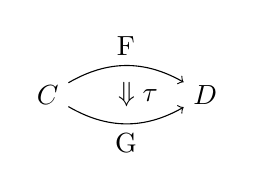
\begin{tikzpicture}
    \node (C) at (-1,0) {$\cat{C}$};
    \node (D) at (1,0) {$\cat{D}$};
    \node (T) at (0,0) {$\;\;\;\Downarrow\tau$};
    \draw[->,bend left] (C) to node [above] {F} (D);
    \draw[->,bend right] (C) to node [below] {G} (D);
  \end{tikzpicture}
\]
such that:
\begin{enumerate}
  \item $\forall X \in \cat{C},
    \exists \tau_X : F(X) \rightarrow G(X) \in \cat{D}$
  \item $\forall f : X \rightarrow Y \in \cat{C},
    \tau_Y \circ F(f) = G(f) \circ \tau_X$
\end{enumerate}
where the Morphism $\tau_X$ is called the \emph{Component} of $\tau$
at $X$. When (2) holds, a Commutative Diagram is formed and the
Morphisms $\tau_X$ are said to be \emph{Natural} in $X$. If there is
no Morphism in $\cat{D}$ corresponding to $\tau_X$, then there can
be no Natural Transformation from $F$ to $G$.

Milewski: A Natural Transformation maps Morphisms to Commuting
Diagrams

When every Component in $\tau$ is Invertible in $\cat{D}$, $\tau$ is a
\emph{Natural Isomorphism} (\S\ref{sec:natural_isomorphism}) and $F
\cong G$. Equivalently, a Natural Isomorphism is an Isomorphism in the
Functor Category $Fun(\cat{C},\cat{D})$.

Natural Isomorphisms:
\[
  Hom_\cat{Grp}(F_1,G) \cong U(G)
\]\[
  Hom_\cat{Set}(X,\cat{2}) \cong \pow(X)
\]\[
  Hom_\cat{BA}(B,\cat{2}) \cong Ult(X)
\]

in Programming Languages, Natural Transformations may be represented
as Polymorphic Functions (i.e. Family of Functions Parameterized by
Types)

Horizontal Composition (\S\ref{sec:horizontal_composition}):
Composition along $1$-morphisms (Functors)

Vertical Composition (\S\ref{sec:horizontal_composition}):
Composition along Objects (Categories)



% ------------------------------------------------------------------------------
\subsection{Vertical Composition}\label{sec:vertical_composition}
% ------------------------------------------------------------------------------

Given Natural Transformations $\eta : F \Rightarrow G$ and $\epsilon :
G \Rightarrow H$ between Functors $F,G,H : \cat{C} \rightarrow
\cat{D}$, the \emph{Vertical Composition} is $\epsilon\circ\eta : F
\Rightarrow H$:
\[
  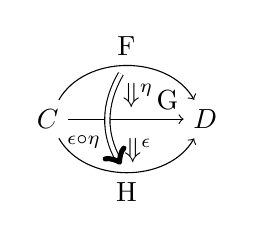
\begin{tikzpicture}
    \node (C) at (-1,0) {$\cat{C}$};
    \node (D) at (1,0) {$\cat{D}$};
    \node (N) at (0,0.3) {$\;\;\;\Downarrow^\eta$};
    \node (M) at (0,-0.4) {$\;\;\;\Downarrow^\epsilon$};
    \node (F) at (0,0.7) {};
    \node (H) at (0,-0.7) {};
    \draw[->,bend left=60] (C) to node [above] {F} (D);
    \draw[->] (C) to node [above] {\quad\quad\quad G} (D);
    \draw[->,bend right=60] (C) to node [below] {H} (D);
    \draw[->,bend right=30,double distance=1.5pt] (F) to
      node [left,pos=0.75] {$_{\epsilon\circ\eta}$} (H);
  \end{tikzpicture}
\]

Composition in the corresponding Functor Category



% ------------------------------------------------------------------------------
\subsection{Horizontal Composition}\label{sec:horizontal_composition}
% ------------------------------------------------------------------------------

Given Functors $F,G : \cat{C} \rightarrow \cat{D}$ and $J,K : \cat{D}
\rightarrow \cat{E}$, and Natural Transformations $\eta : F
\rightarrow G$ and $\epsilon : J \rightarrow K$, the \emph{Horizontal
  Composition} (or \emph{Godement Product}) is $\eta * \epsilon : JF
\Rightarrow KG$:
\[
  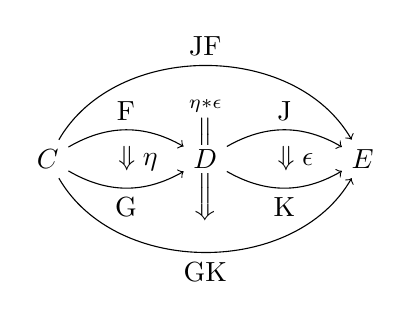
\begin{tikzpicture}
    \node (U) at (0,0) {$\stackrel{\eta*\epsilon}
      {\stackrel{\Big\|}{\Big\Downarrow}}$};
    \node [fill,color=white,scale=1.5] (W) at (0,0) {};
    \node (C) at (-2,0) {$\cat{C}$};
    \node (D) at (0,0) {$\cat{D}$};
    \node (E) at (2,0) {$\cat{E}$};
    \node (S) at (-1,0) {$\;\;\;\Downarrow\eta$};
    \node (T) at (1,0) {$\;\;\;\Downarrow\epsilon$};
    \draw[->,bend left] (C) to node [above] {F} (D);
    \draw[->,bend right] (C) to node [below] {G} (D);
    \draw[->,bend left] (D) to node [above] {J} (E);
    \draw[->,bend right] (D) to node [below] {K} (E);
    \draw[->,bend left=60] (C) to node [above] {JF} (E);
    \draw[->,bend right=60] (C) to node [below] {GK} (E);
  \end{tikzpicture}
\]

Horizontal Composition is Associative and has the same Identity as
Vertical Composition.



% ------------------------------------------------------------------------------
\subsection{Interchange Law}\label{sec:interchange_law}
% ------------------------------------------------------------------------------

Given three Categories, $\cat{B}$, $\cat{C}$, and $\cat{D}$,
and six Functors, $P,Q,R : \cat{B} \rightarrow \cat{C}$ and
$S,T,U : \cat{C} \rightarrow \cat{D}$, and four Natural
Transformations, $\sigma : P \rightarrow Q$, $\tau : Q \rightarrow R$,
$\sigma' : S \rightarrow T$, and $\tau' : T \rightarrow U$, the
following \emph{Interchange Law} applies:
\[
  (\tau' \cdot \sigma') \circ (\tau \cdot \sigma) =
  (\tau' \circ \tau) \cdot (\sigma' \circ \sigma)
\]



% ------------------------------------------------------------------------------
\subsection{Natural Isomorphism}\label{sec:natural_isomorphism}
% ------------------------------------------------------------------------------

\emph{Natural Equivalence} in a $1$-category %FIXME xref

\[
  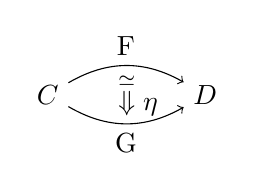
\begin{tikzpicture}
    \node (C) at (-1,0) {$\cat{C}$};
    \node (D) at (1,0) {$\cat{D}$};
    \node (N) at (0,0) {$\;\;\;\stackrel{\simeq}{\Downarrow}\eta$};
    \draw[->,bend left] (C) to node [above] {F} (D);
    \draw[->,bend right] (C) to node [below] {G} (D);
  \end{tikzpicture}
\]

\begin{itemize}
  \item Natural Isomorphism with a Two-sided Inverse (???)
  \item each Component $\eta_X : F(X) \rightarrow G(X)$ for all $X
    \in \cat{C}_0$ is an Isomorphism in $\cat{D}$
  \item Isomorphism in the Functor Category
    (\S\ref{sec:functor_category}) $[\cat{C},\cat{D}]$
\end{itemize}



% ------------------------------------------------------------------------------
\subsection{Extranatural Transformation}
\label{sec:extranatural_transformation}
% ------------------------------------------------------------------------------

For Functors $F : \cat{A} \times \cat{B}^{op} \times \cat{B}
\rightarrow \cat{D}$ and $G : \cat{A} \times \cat{C}^{op} \times
\cat{C} \rightarrow \cat{D}$, the Family $\eta(a,b,c) : F(a,b,b)
\rightarrow G(a,c,c)$ is Natural in $a$ and \emph{Extranatural} in $b$
and $c$ if the following holds:
\begin{itemize}
  \item (Natural in $a$): $\eta (-,b,c)$ is a Natural Transformation
  \item (Extranatural in $b$): $\forall (g:b \rightarrow b') \in
    \cat{B}_1, \forall a \in \cat{A}, \forall c \in \cat{C},
    \eta(a,b,c) \circ F(1,1,g) = \eta(a,b',c) \circ F(1,g,1)$
  \item (Extranatural in $c$): $\forall (h:c \rightarrow c') \in
    \cat{C}_1, \forall a \in \cat{A}, \forall b \in \cat{B}, G(1,h,1)
    \circ \eta(a,b,c) = G(1,1,h) \circ \eta(a,b,c')$
\end{itemize}



% ------------------------------------------------------------------------------
\subsection{Dinatural Transformation}
\label{sec:dinatural_transformation}
% ------------------------------------------------------------------------------

Ex.: Hughes Arrow (\S\ref{sec:hughes_arrow}) $\ggg : A (X,P) \times A
(P,Y) \rightarrow A (X,Y)$ is Dinatural in $P$. For each $f : P
\rightarrow Q$:
\[
  id \times A(f,id) \circ \ggg = A(id,f) \times id \circ \ggg
\]



% ==============================================================================
\section{Opposite Category}\label{sec:opposite_category}
% ==============================================================================

The \emph{Opposite} or \emph{Dual} (\S\ref{sec:abstract_category})
of a Category $\cat{C}$ is denoted $\cat{C^{op}}$ or
$\cat{C^*}$ and has the same Objects as $\cat{C}$ but the Domain
and Codomain in each Morphism is reversed. Objects and Morphisms of a
Dual Category may be written with over-lines to distinguish them from
the original Category: $\overline{f}: \overline{C} \rightarrow
\overline{D}$. With this notation the following Equalities may be
expressed:
\[
  1_{\overline{C}} = \overline{1_C}
\]\[
  \overline{f} \circ \overline{g} = \overline{g \circ f}
\]
A Terminal Object in $\cat{C}$ is an Initial Object in
$\cat{C^{op}}$ and vice-versa.

The Functor $(-)^\cat{op} : \cat{Cat} \rightarrow \cat{Cat}$
is an Involution (\S\ref{sec:involution}) but is Contravariant so it
does not define any Isomorphisms.

In a Dual Category the following are all Duals of eachother:
\begin{itemize}
  \item Monomorphisms and Epimorphisms (\S\ref{sec:morphism})
  \item Left and Right Inverses (\S\ref{sec:morphism})
  \item Initial and Terminal Objects (\S\ref{sec:universal_property})
\end{itemize}



% ==============================================================================
\section{Category Product}\label{sec:category_product}
% ==============================================================================

A \emph{Category Product}, $\times$, is a Construction (i.e. a Functor,
specifically a Bifunctor \S\ref{sec:bifunctor}) on Categories (or
Functors):
\[
  \times : \cat{Cat} \times \cat{Cat} \rightarrow \cat{Cat}
\]

This operation is the Cartesian Product (\S\ref{sec:product}) in the
$1$-category $\cat{Cat}$



% ------------------------------------------------------------------------------
\subsection{Product Category}\label{sec:product_category}
% ------------------------------------------------------------------------------

A \emph{Product Category} can be constructed from two Categories,
$\cat{C}$ and $\cat{D}$, and is denoted:
\[
  \cat{C} \times \cat{D}
\]
has Objects of the form $(C,D)$ where $C \in \cat{C}$ and $D \in
\cat{D}$ and Morphisms $(f,g) : (C,D) \rightarrow (C',D')$ where $f
: C \rightarrow C' \in \cat{C}$ and $g : D \rightarrow D' \in
\cat{D}$. Composition and Identity are defined as:
\[
  (f',g') \circ (f,g) = (f' \circ f,g' \circ g)
\]\[
  1_{(C,D)} = (1_C, 1_D)
\]
$\cat{C} \times \cat{D}$ is a Product (\S\ref{sec:product}) in
$\cat{Cat}$.



\subsubsection{Projection}\label{sec:projection_functor}

A Product Category has a pair of \emph{Projections} which are Functors
from the Product Category to the original Categories:
\[
  \cat{C} \xleftarrow{\;\; P\;\;} \cat{C}\times\cat{D}
  \xrightarrow{\;\; Q\;\;} \cat{D}
\]
such that for $C,f \in \cat{C}, D,g \in \cat{D}$:
\[
  P(C,D) = C, \;\; P(f,g) = f
\]\[
  Q(C,D) = D, \;\; Q(f,g) = g
\]
Given any other Category, $\cat{B}$, there exists a unique Functor:
\[
  F : \cat{B} \rightarrow \cat{C} \times \cat{D}
\]
with:
\[
  PF = R : \cat{B} \rightarrow \cat{C}
\]\[
  QF = T : \cat{B} \rightarrow \cat{D}
\]
giving:
\[
  \forall h \in B, F(h) = (Rh,Th)
\]



% ------------------------------------------------------------------------------
\subsection{Functor Product}\label{sec:functor_product}
% ------------------------------------------------------------------------------

Give two Functors, $U : \cat{C} \rightarrow \cat{C'}$ and $V :
\cat{D} \rightarrow \cat{D'}$, a \emph{Functor Product} is
defined as:
\[
  U \times V : \cat{C} \times \cat{D}
  \rightarrow \cat{C'} \times \cat{D'}
\]
where:
\[
  (U \times V)(C,D) = (UC,VD), \;\; (U \times V)(f,g) = (Uf,Vg)
\]
and $(U \times V)$ is the unique Functor such that:
\[
  P'(U \times V) = UP, \;\; Q'(U \times V) = VQ
\]
%FIXME is the above correct?



% ==============================================================================
\section{Quotient Category}\label{sec:quotient_category}
% ==============================================================================

%FIXME this probably needs a rewrite

The \emph{Quotient Category} is defined for a Category $\cat{C}$
with Congruence Relation $\sim$ as $\cat{C}/\sim$:
\[
  (\cat{C}/\sim)_0 = \cat{C_0}
\]\[
  (\cat{C}/\sim)_1 = (\cat{C_1})/\sim
\]
where Morphisms are of the form $[f]$ where $f \in \cat{C_1}$.

For a Category $\cat{C}$ with Graph $G$ and relations $R$,
$\cat{C}/R$ is called the Category with \emph{Generators} $G$ and
\emph{Relations} $R$.

Homotopy Category (\S\ref{sec:homotopy_category})



% ------------------------------------------------------------------------------
\subsection{Congruence Category}\label{sec:congruence_category}
% ------------------------------------------------------------------------------

\emph{Congruence} on a Category is an Equivalence Relation on
Morphisms such that for two Morphisms $f,g \in \cat{C_1}$, $f \sim
g$ Implies:
\begin{itemize}
  \item $dom(f) = dom(g)$
  \item $cod(f) = cod(g)$
  \item $\forall a,b \in \cat{C_1}, bfa \sim bga$
\end{itemize}
Such a Congruence defines a \emph{Congruence Category}
$\cat{C^{\sim}}$:
\[
  (\cat{C^{\sim}})_0 = \cat{C}_0
\]\[
  (\cat{C^{\sim}})_1 = \{\langle f,g \rangle | f \sim g\}
\]\[
  \tilde{1_\cat{C}} = \langle 1_\cat{C}, 1_\cat{C} \rangle
\]\[
  \langle f',g' \rangle \circ \langle f,g \rangle = \langle f'f,g'g \rangle
\]
The Categorical Congruence $\sim$ on a Group $G$ is a Normal Subgroup
$N \subseteq G$ and the Quotient Category $G/\sim$ and the Quotient
Group $G/N$ coincide. \cite{awodey06}



% ------------------------------------------------------------------------------
\subsection{Kernel Category}\label{sec:kernel_category}
% ------------------------------------------------------------------------------

Given a Functor $F : \cat{C} \rightarrow \cat{D}$, a Congruence
$\sim_F$ on $\cat{C}$ is defined as:
\[
  f \sim_F g \leftrightarrow dom(f) = dom(g) \wedge cod(f) = cod(g)
  \wedge F(f) = F(g)
\]
The \emph{Kernel Category} of $F$ is then defined as the Congruence
Category of $\sim_F$
\[
  ker(F) = C^{\sim_F}
\]



% ------------------------------------------------------------------------------
\subsection{Finitely Presented Category}
\label{sec:finitely_presented}
% ------------------------------------------------------------------------------

% FIXME free category notation?
A \emph{Finitely Presented Category} is given by taking the Quotient
Category of a Free Category (\S\ref{sec:free_category})
$\cat{C}(G)$ with the Congruence $\sim_\Sigma$:
\[
  \cat{C}(G) / \sim_{\Sigma} = \cat{C}(G,\Sigma)
\]
where $\Sigma$ is the finite Set of Relations:
\[
  (g_1 \circ \ldots \circ g_n) = (g'_1 \circ \ldots \circ g'_m)
\]
for all $g_i \in G$ such that $dom(g_n) = dom(g'_m)$ and $cod(g_1) =
cod(g'_1)$.

\fist Locally Presentable Category (\S\ref{sec:locally_presentable})



% ==============================================================================
\section{Comma Category}\label{sec:comma_category}
% ==============================================================================

A \emph{Comma Category} is formed from a pair of Functors that share a
common Codomain. For three Categories, $\cat{A}$, $\cat{B}$, and
$\cat{C}$ and Functors $S$ (\emph{Source}) and $T$ (\emph{Target}) in
the following relation:
\[
  \cat{A} \xrightarrow{\;\; S\;\;} \cat{C} \xleftarrow{\;\;
    T\;\;} \cat{B}
\]
one can form a Comma Category $(S \downarrow T)$ with Objects as
Triples $(\alpha, \beta, f)$ where $\alpha$ is an Object in
$\cat{A}$, $\beta$ is an Object in $\cat{B}$, and $f : S(\alpha)
\rightarrow T(\beta)$ is a Morphism in $\cat{C}$ and with Morphisms
between Triples $(\alpha, \beta, f)$ to $(\alpha', \beta', f')$ as
pairs $(g,h)$ where $g : \alpha \rightarrow \alpha'$ is a Morphism in
$\cat{A}$ and $h : \beta \rightarrow \beta'$ is a Morphism in
$\cat{B}$.

When $S$ is a Functor, $\cat{1} \xrightarrow{\;\;S\;\;}
\cat{C}$, to a single Object $A \in \cat{C}$, the resulting
Comma Category may be denoted $(A \downarrow \cat{C})$ and is
called the Category of Objects under $A$. Here Objects are Morphisms
with Domain of $A$, and Morphisms are Commutative triangles with top
Vertex $A$.

The Category of Objects over $A$ is likewise $(\cat{C} \downarrow
A)$ and has as Objects Morphisms with Codomain $A$ and Morphisms are
Commutative triangles with a bottom Vertex $A$.

When both $S$ and $T$ are Functors from $\cat{1}$ to Objects $A$
and $B$ respectively, the result is a Discrete Category whose Objects
are $Hom(A,B)$.

The case where $S = T = 1_\cat{C}$, $(\cat{C} \downarrow
\cat{C})$, is the Category of all Morphisms of $\cat{C}$:
$\cat{C}^\cat{2}$.



% ------------------------------------------------------------------------------
\subsection{Arrow Category}\label{sec:arrow_category}
% ------------------------------------------------------------------------------

An \emph{Arrow Category} of a Category $\cat{C}$, written
$\cat{C^{\rightarrow}}$, has for its Objects the Morphisms of
$\cat{C}$ and as Morphisms pairs of Objects such that their
underlying Morphisms in $\cat{C}$ are Composable (Commutative
Squares).

Equivalent to the Comma Category $(1_\cat{C}/1_\cat{C})$

The Arrow Category $\cat{C}^\rightarrow$ is Isomorphic to the
Functor Category $\cat{C^2}$.

There are two Functors defined on an Arrow Category:
\[
  \cat{C} \xleftarrow{\cat{dom}} \cat{C}^\rightarrow
  \xrightarrow{\cat{cod}} \cat{D}
\]



% ------------------------------------------------------------------------------
\subsection{Slice Category}\label{sec:slice_category}
% ------------------------------------------------------------------------------

A \emph{Slice Category} (or \emph{Overcategory}) $\cat{C}/C$ of a
Category $\cat{C}$ with an Object $C$ has as Objects the Morphisms
with Codomain $C$ and as Morphisms those Morphisms in $\cat{C}$
between the Domains of the underlying Morphisms of the Objects of
$\cat{C}/C$. That is, for Objects in the Slice Category corresonding
to Morphisms $f$ and $f'$, the Morphism in the Slice Category between
the two is $g$ such that
\[
  f' \circ g = f
\]

\emph{Coslice}

if each Slice Category $\cat{C}/x$ is a Cartesian Monoidal Category
(\S\ref{sec:cartesian_monoidal}) then $\cat{C}$ is Locally Cartesian
(\S\ref{sec:locally_cartesian})

Categorical Semantics (\S\ref{sec:categorical_semantics}) for Formal
Logic (Part \ref{part:formal_logic}) and Type Theory (Part
\ref{part:type_theory})



% ------------------------------------------------------------------------------
\subsection{Coslice Category}\label{sec:coslice_category}
% ------------------------------------------------------------------------------



% ==============================================================================
\section{Bifunctor}\label{sec:bifunctor}
% ==============================================================================

A \emph{Bifunctor} is a Functor of two Variables from a Product
Category to an arbitrary Category:
\[
  B : \cat{C} \times \cat{D} \rightarrow \cat{A}
\]

A \emph{Multifunctor} is a generalized to $n$ or more Variables.



% ------------------------------------------------------------------------------
\subsection{Product Functor}\label{sec:product_functor}
% ------------------------------------------------------------------------------

\[
  \times : \cat{C} \times \cat{C} \rightarrow \cat{C}
\]

Category Product (\S\ref{sec:category_product})



% ------------------------------------------------------------------------------
\subsection{Coproduct Functor}\label{sec:coproduct_functor}
% ------------------------------------------------------------------------------

\[
  + : \cat{C} \times \cat{C} \rightarrow \cat{C}
\]



% ------------------------------------------------------------------------------
\subsection{Diagonal Functor}\label{sec:diagonal_functor}
% ------------------------------------------------------------------------------

For Functor Category (\S\ref{sec:functor_category})
$\cat{C}^\cat{J}$ with Small Index Category $\cat{J}$, a
\emph{Diagonal Functor} $\Delta : \cat{C} \rightarrow
\cat{C}^\cat{J}$ assigns to each Object $A$ of $\cat{C}$ the
Constant Functor $\Delta_A \in \cat{C}^\cat{J}$ with fixed $A$
and to each Morphism $f : A \rightarrow B$ of $\cat{C}$ the Natural
Transformation $\eta$ in $\cat{C}^\cat{J}$ given by $\eta_j =
f$.

If $\cat{J}$ is a Discrete Category with two Objects, the Diagonal
Functor is $\cat{C} \rightarrow \cat{C} \times \cat{C}$.

The Limit (\S\ref{sec:limit}) of a Functor $F : \cat{J} \rightarrow
\cat{C}$ is a Universal Morphism (\S\ref{sec:universal_morphism})
from the Diagonal Functor $\Delta$ to $F$.

If $\cat{C}$ is Complete (\S\ref{sec:complete_category}) then every
Functor from $\cat{J}$ to $\cat{C}$ has a Limit and the
operation of taking Limits is a Functor from $\cat{C}^\cat{J}$
to $\cat{C}$.

The Limit Functor is the Right-adjoint (\S\ref{sec:adjoint_functor})
of the Diagonal Functor.

A Colimit (\S\ref{sec:colimit}) is a Universal Morphism $F \rightarrow
\Delta$.

If $\cat{C}$ is Complete the Colimit Functor exists and is the
Left-adjoint of the Diagonal Functor.

As an example, the Diagonal Functor $\cat{C} \rightarrow \cat{C}
\times \cat{C}$ is the Left-adjoint of the Binary Product Functor
(\S\ref{sec:product_functor}) and the Right-adjoint of the Binary
Coproduct Functor (\S\ref{sec:coproduct_functor}).



% ------------------------------------------------------------------------------
\subsection{Profunctor}\label{sec:profunctor}
% ------------------------------------------------------------------------------

A \emph{Profunctor} (or \emph{Distributor}) is a Bifunctor that is
Contravariant in the first argument and Covariant in the second.

Generalization of Functors, Categorical generalization of Bimodules
(\S\ref{sec:bimodule})

\url{https://golem.ph.utexas.edu/category/2018/02/cartesian_bicategories.html}:
``A Profunctor from $\cat{C}$ to $\cat{D}$ is a Functor from $\cat{D}^{op}
\times \cat{C}$ to $\cat{Set}$ ... Heuristically, Profunctors can be thought of
as a generalization of Relations when considering Profunctors as
`$\cat{Set}$-valued Matrix of size $ob(\cat{C} \times ob(\cat{D})$'''

$P : \cat{C} \nrightarrow \cat{D}$

$H_P : \cat{D}^{op} \times \cat{C} \rightarrow \cat{Set}$

Set of Heteromorphisms (\S\ref{sec:heteromorphism})

Identity Profunctor $Id : \cat{C} \nrightarrow \cat{C}$ is given by
the Hom-functor $\cat{C}(-,-) : \cat{C}^{op} \times \cat{C}
\rightarrow \cat{Set}$

Composition of Profunctors $P : \cat{C} \nrightarrow \cat{D}$, $Q :
\cat{D} \nrightarrow \cat{E}$:
\[
  Q P = \int^{d \in \cat{D}} P(d,-) \otimes Q(-,d)
\]
% FIXME kan extensions?

Every Functor $F : \cat{C} \rightarrow \cat{D}$ induces two
Profunctors $D(1,F) : \cat{C} \nrightarrow \cat{D}$ and $D(F,1)
: \cat{D} \nrightarrow \cat{C}$ where $D(1,F)(d,c) = D(d,f(c))$
and $D(f,1)(c,d) = D(f(c),d)$.

Functor $F : \cat{C} \rightarrow \cat{D}$ gives a Profunctor $P_F :
\cat{C} \nrightarrow \cat{D}$ by Post-composition with the Yoneda
Functor (\S\ref{sec:yoneda_embedding}):
\[
  P_F = Y_\cat{D} \circ F
\]



\subsubsection{Profunctor Bicategory}\label{sec:profunctor_bicategory}

Bicategory (\S\ref{sec:bicategory}) of Profunctors

Coend (\S\ref{sec:coend})



% ==============================================================================
\section{Hom-functor}\label{sec:hom_functor}
% ==============================================================================

A \emph{Hom-functor} is a Functor from a Locally Small Category
(\S\ref{sec:locally_small}), $\cat{C}$, to the Category $\cat{Set}$,
and has a Covariant and a Contravariant definition:

\begin{enumerate}
  \item \emph{Covariant Hom-functor}, for $A \in \cat{C}_0$, $f : X
    \rightarrow Y \in \cat{C}_1$:
\[
\begin{split}
  & h^A = Hom(A,-) : \cat{C} \rightarrow \cat{Set} \\
  & X \mapsto Hom(A,X) \\
  & f \mapsto Hom(A,f) : Hom(A,X) \rightarrow Hom(A,Y)
\end{split}
\]
  where $Hom(A,f)$ is defined for all $g \in Hom(A,X)$ as:
\[
  g \mapsto f \circ g
\]

  \item \emph{Contravariant Hom-functor} (also \emph{Functor of
    Points}, see Generalized Elements
    \S\ref{sec:generalized_element}), for $B \in \cat{C}_0$, $f : X
    \rightarrow Y \in \cat{C}_1$:
\[
\begin{split}
  & h_B = Hom(-,B) : \cat{C} \rightarrow \cat{Set} \\
  & X \mapsto Hom(X,B) \\
  & f \mapsto Hom(f,B) : Hom(Y,B) \rightarrow Hom(X,B)
\end{split}
\]
  where $Hom(f,B)$ is defined for all $g \in Hom(Y,B)$ as:
\[
  g \mapsto g \circ f
\]
\end{enumerate}

The Hom-functor $Hom(-,-)$ is a Covariant Bifunctor
(\S\ref{sec:bifunctor}):
\[
  Hom_\cat{C}(-,-):
    \cat{C}^{op} \times \cat{C} \rightarrow \cat{Set}
\]
each half of which is a Representable Functor
(\S\ref{sec:representable_functor}). $Hom_\cat{C}(-,-)$ is also the
Identity Profunctor (\S\ref{sec:profunctor}) $1_\cat{C} :
\cat{C} \nrightarrow \cat{C}$. Hom-functors are Continuous
Functors (\S\ref{sec:continuous_functor}).

The Category of all Hom-functors and Natural Transformations
(\S\ref{sec:natural_transformation}) between them, $\{ h^A | A \in
\cat{C} \}$, is a Subcategory of the Functor Category
(\S\ref{sec:functor_category}) $\cat{Set^C}$, and is Isomorphic to
$\cat{C^{op}}$ (see Yoneda Embedding \S\ref{sec:yoneda_embedding}).

Every Morphism $f : A' \rightarrow A$ determines a pair of Natural
Transformations:
\[
  Hom(f,-) : h^A \rightarrow h^{A'}
\]\[
  Hom(-,f) : h_{A'} \rightarrow h_A
\]

For any pair of Morphisms, $f : A' \rightarrow A$ and $g : B
\rightarrow B'$:
\[
  Hom(A',g) \circ Hom(f,B) = Hom(f,B') \circ Hom(A,g)
\]
is a path sending:
\[
  h : A \rightarrow B
\]
to:
\[
  g \circ h \circ f : A' \rightarrow B'
\]



% ------------------------------------------------------------------------------
\subsection{Closed Category}\label{sec:closed_category}
% ------------------------------------------------------------------------------

A \emph{Closed Category} is a Category $\cat{C}$ with:
\begin{itemize}
  \item Internal Hom-functor (\S\ref{sec:internal_hom}):
    \[
      [-,-]:\cat{C}^{op} \times \cat{C} \rightarrow \cat{C}
    \]
  \item Unit Object:
    \[
      I \in \cat{C}_0
    \]
  \item Natural Isomorphism:
    \[
      i : 1_\cat{C} \cong [I,-]
    \]
  \item Transformation:
    \[
      j_X : I \rightarrow [X,X]
    \]
    Extranatural (\S\ref{sec:extranatural_transformation}) in $X$
  \item Transformation:
    \[
      L_{Y Z}^X : [Y,Z] \rightarrow [[X,Y],[X,Z]]
    \]
    Natural in $Y$ and $Z$ and Extranatural in $X$
\end{itemize}
Satisfying the Axioms:
\begin{enumerate}
  \item $L_{Y Y}^X \circ j_Y = j_{[X,Y]}$ for any $X,Y$
  \item $[j_X,1] \circ L_{X Y}^X = i_{[X,Y]}$ for any $X,Y$
  \item $[i_Y,1] \circ L_{Y Z}^I = [1,i_Z]$ for any $Y,Z$
  \item $[1,L_{Y V}^X] \circ L_{U V}^Y = [L_{Y U}^X,1] \circ L_{[X,U]
    [X,V]}^{[X,Y]} \circ L_{U V}^X$ for any $X,Y,U,V$
  \item The Map $\gamma : \cat{C}(X,Y) \rightarrow \cat{C}(I,[X,Y])$
    defined by $f \mapsto [1,f](j_X)$ is a Bijection
\end{enumerate}

Every Closed Category embeds Fully and Faithfully into a Closed
Monoidal Category (\S\ref{sec:closed_monoidal}) by a Strong Closed
Functor (LaPlaza) %FIXME



\subsubsection{Internal Hom-functor}\label{sec:internal_hom}

\emph{Internal Hom Functor}
\[
  [-,-] : \cat{C}^{op} \times \cat{C} \rightarrow \cat{C}
\]

examples:
\begin{itemize}
  \item (nlab): in the ``Context'' $H$ (FIXME: clarify) of Synthetic
    Differential Geometry (\S\ref{sec:synthetic_differential_geometry}), the
    Differentiation (\S\ref{sec:derivative}) (Endo-)functor $\mathrm{d} :
    \cat{Diff} \rightarrow \cat{Diff}$ on the Category of Smooth Manifolds and
    Smooth Maps is the Internal Hom out of the Infinitesimal Interval
    (\S\ref{sec:infinitesimal_interval}) $D$:
    \[
      \mathrm{d} = [D,-] : H \rightarrow H
    \]
    where $D \hookrightarrow \reals$ is the Smooth Locus (FIXME: xref) defined
    by $x^2 = 0$ (in Toposes that Model Synthetic Differential Geometry this is
    regarded as an Infinitesimal Neighborhood about a Point)
  \item ... TODO: more
\end{itemize}



\subsubsection{Dualizing Object}\label{sec:dualizing_object}

\emph{Dualizing Object} $D$ in a Closed Category $\cat{D}$ is an
Object with Internal Hom $[-,D]: \cat{C} \rightarrow \cat{C}^{op}$, an
Involutive Duality Operation on $\cat{C}$: %FIXME
\[
  [[-,D],D]: \cat{C} \rightarrow \cat{C}
\]

Dual Object (\S\ref{sec:dual_object})



\subsubsection{Symmetric Closed Category}
\label{sec:symmetric_closed_category}

BCI Combinators (\S\ref{sec:bci_logic}) have the Types of the basic
Operations in a Symmetric Closed Category



\subsubsection{Doubly Closed Category}\label{sec:doubly_closed_category}

Category with two Monoidal Closed Structures

Cartesian if one of the Closed Structures is Cartesian and the other
Symmetric Monoidal and Bicartesian if also has Finite Coproducts



\paragraph{Cartesian Doubly Closed Category}
\label{sec:cartesian_doubly_closed}\hfill

Doubly Closed Category where one of the Closed Structures is Cartesian
and the other is Symmetric Monoidal



\paragraph{Bicartesian Doubly Closed Category}
\label{sec:bicartesian_doubly_closed}\hfill

Cartesian Doubly Closed Category with Finite Coproducts

Categorical Semantics of Logic of Bunched Implications
(\S\ref{sec:bunched_logic})



% ------------------------------------------------------------------------------
\subsection{Representable Functor}\label{sec:representable_functor}
% ------------------------------------------------------------------------------

%FIXME definition of 'representation'
%FIXME ref Naturally Isomorphic
Presheaf (\S\ref{sec:category_presheaf})

A Functor $F : \cat{C} \rightarrow \cat{Set}$ is a
\emph{Representable Functor} if it is Naturally Isomorphic to the
Hom-functor $h^A$ or $h_A$ for some Object $A \in \cat{C}$.

A \emph{Covariant Representable Functor} for an Object $A$ in a
Category $\cat{C}$ is defined as Naturally Isomorphic to the
Covariant Hom-functor $h^A = Hom(A,-) : \cat{C} \rightarrow
\cat{Set}$
\[
  Hom(A,-) : Hom(A,X) \xrightarrow{f_*} Hom(A,Y)
\]
A \emph{Contravariant Representable Functor} for $A$ is a Functor that
is Naturally Isomorphic to the Contravariant Hom-functor $h_A =
Hom(-,A) : \cat{C^{op}} \rightarrow \cat{Set}$
\[
  Hom(-,A) : Hom(X,A) \xrightarrow{f^*} Hom(Y,A)
\]

A \emph{Representation} of a Covariant Representable Functor, $F$, is
a pair $(A, \Phi)$ with Natural Isomorphism $\Phi : Hom(A,-)
\rightarrow F$.

Contravariant Representable Functors map all Colimits
(\S\ref{sec:colimit}) to Limits (\S\ref{sec:limit}).

A Locally Small Category (\S\ref{sec:locally_small}) has Representable
Functors for all Objects.

generalization of Upper Sets (\S\ref{sec:upper_set}) in Posets



% ------------------------------------------------------------------------------
\subsection{Locally Small Category}\label{sec:locally_small}
% ------------------------------------------------------------------------------

A Category is \emph{Locally Small} if all Hom-sets
(\S\ref{sec:hom_set}) of the Category are Sets and not Proper Classes.
% FIXME definition in terms of hom-sets

Hom-functor (\S\ref{sec:hom_functor})

There is at least one canonical Representable Functor
(\S\ref{sec:representable_functor}) from any Locally Small Category
into $\cat{Set}$.

For a Locally Small Category $\cat{C}$, $\cat{Set^{C^{op}}}$ is
Complete (\S\ref{sec:complete_category}) and Cocomplete
(\S\ref{sec:cocomplete_category}) and for all $C \in \cat{C}_0$,
the Evaluation Functor $ev_C : \cat{Set^{C^{op}}} \rightarrow
\cat{Set}$ preserves all Limits. \cite{awodey06}



% ==============================================================================
\section{Concrete Category}\label{sec:concrete_category}
% ==============================================================================

A \emph{Concrete Category} is pair, $(\cat{C},U)$, where $\cat{C}$ is
a Category and $U$ is a Faithful Functor
(\S\ref{sec:faithful_functor}) $U : \cat{C} \rightarrow \cat{Set}$.

Representable Functor (\S\ref{sec:representable_functor})

Sets with Structure (\S\ref{sec:abstract_structure})

Categories with Interpretations as Concrete Categories:
\begin{itemize}
  \item $\cat{Set}$
  \item $\cat{Top}$
  \item $\cat{Grp}$
\end{itemize}

Not \emph{Concretizable}:
\begin{itemize}
  \item $\cat{Toph}$
\end{itemize}



% ==============================================================================
\section{Yoneda Lemma}\label{sec:yoneda_lemma}
% ==============================================================================

For an arbitrary Covariant Functor $F : \cat{C} \rightarrow
\cat{Set}$:
\[
  Nat_\cat{Set^C}(h^A,F) \cong F(A)
\]
If $F$ is a Covariant Hom-functor $h^B$, then:
\[
  Nat_\cat{Set^C}(h^A,h^B) \cong Hom(B,A)
\]

For an arbitrary Contravariant Functor $G : \cat{C}^{op} \rightarrow
\cat{Set}$:
\[
  Nat_\cat{Set^{C^op}}(h_B,G) \cong G(A)
\]
If $F$ is a Contravariant Hom-functor $h_B$, then:
\[
  Nat_\cat{Set^{C^{op}}}(h_A,h_B) \cong Hom(A,B)
\]

Corollary:
\[
  yA \cong yB \Rightarrow A \cong B
\]



% ------------------------------------------------------------------------------
\subsection{Yoneda Embedding}\label{sec:yoneda_embedding}
% ------------------------------------------------------------------------------

The Fully Faithful Contravariant Functor $h^- : \cat{C} \rightarrow
\cat{Set^C}$ which maps each Object $A \in \cat{C}_0$ to the
Hom-functor $h^A$ and each $f \in \cat{C}_1$ to the Natural
Transformation $Hom(f,-)$ can also be interpreted as a Covariant
Functor $h^- : \cat{C^{op}} \rightarrow \cat{Set^C}$. Being a
Faithful Functor means $h^-$ gives an Embedding
(\S\ref{sec:category_embedding}) of $\cat{C^{op}}$ in
$\cat{Set^C}$.

By the Contravariant Yoneda's Lemma:
\[
  h_-: \cat{C} \rightarrow \cat{Set^{C^{op}}}
\]
called the \emph{Yoneda Embedding}.

Covariant:

$Nat_\cat{Set^C}(Hom(A,-), Hom(B,-)) \cong Hom_\cat{C}(B,A)$

Contravariant:

$Nat_\cat{Set^{C^op}}(Hom(-,A), Hom(-,B)) \cong Hom_\cat{C}(A,B)$

Yoneda Embedding preserves all Products and Exponentials in
$\cat{C}$.



% ------------------------------------------------------------------------------
\subsection{Coyoneda}\label{sec:coyoneda}
% ------------------------------------------------------------------------------

Free Functor (\S\ref{sec:free_functor})



% ==============================================================================
\section{Functor Category}\label{sec:functor_category}
% ==============================================================================

Given two Categories, $\cat{C}$ and $\cat{D}$, a \emph{Functor
  Category} is a Category with Objects as Functors $T : \cat{C}
\rightarrow \cat{D}$ and Morphisms as Natural Transformations
between Functors:
\[
  \cat{D}^{\cat{C}} = Fun(\cat{C},\cat{D})
\]

$[\cat{C},\cat{D}]$

A Hom-set in a Functor Category may be denoted:
\[
  Nat(S,T) = \cat{D}^{\cat{C}}(S,T) =
    \{ \tau | \tau : S \rightarrow T \}
\]

With Evaluation Functor $\eta : \cat{D^C} \times \cat{C} \rightarrow
\cat{D}$, $\cat{D^C}$ is an Exponential
(\S\ref{sec:category_exponential}) in $\cat{Cat}$ and $\cat{Cat}$ is a
Cartesian Closed Category (\S\ref{sec:cartesian_closed}).

The Functor Category $\cat{C^2}$ is Isomorphic to Arrow Categories
(\S\ref{sec:arrow_category}) $\cat{C}^\rightarrow$.

The Functor Category $\cat{C}^\cat{2}$ from the Discrete Category
$\cat{2}$ is equivalent to the Product Category $\cat{C} \times
\cat{C}$.

For any Discrete Category $I$:
\[
  \cat{C}^I \cong \prod_{i \in I} \cat{C}
\]

The Functor Category $\cat{Set}^\downdownarrows$ where
$\downdownarrows$ is the Category with two Objects and two Morphisms
between them ($* \rightrightarrows \star$) is equivalent to the
Category of Graphs and Graph Homomorphisms $\cat{Graph}$. Cf.
Simplicial Sets (\S\ref{sec:simplicial_set}).

A Functor Category into the Category $\cat{Set}$ is called a
\emph{Category Diagram} (\S\ref{sec:category_diagram}).
%FIXME terminology doesn't match



% ------------------------------------------------------------------------------
\subsection{Set-valued Functor Category}\label{sec:setvalued_functor}
% ------------------------------------------------------------------------------

A \emph{Set-valued Functor Category} (or \emph{Category of Diagrams})
is a Functor Category from a Category into the Category
$\cat{Set}$.

A Presheaf (\S\ref{sec:presheaf}) is an example of a Set-valued
(Contravariant) Functor Category from an Opposite Category into
$\cat{Set}$.



\subsubsection{Powerset Functor}\label{sec:powerset_functor}

$\pow : \cat{Set} \rightarrow \cat{Set}$

Functions $f : X \rightarrow Y$ to the Image Mapping $img(f) :
\pow(X) \rightarrow \pow(Y)$



% ==============================================================================
\section{Presheaf Category}\label{sec:presheaf_category}
% ==============================================================================

Objects: Functors $F: \cat{C}^{op} \rightarrow \cat{Set}$

Morphisms: Natural Transformations $\Phi : F \rightarrow G$

$Psh(\cat{C}) = [\cat{C}^{op},\cat{Set}]$



% ------------------------------------------------------------------------------
\subsection{Presheaf}\label{sec:category_presheaf}
% ------------------------------------------------------------------------------

A \emph{Presheaf} is a Contravariant Functor from an Opposite Category
to the Category $\cat{Set}$. A Presheaf is an example of a
Set-valued Functor Category (\S\ref{sec:category_diagram}) and gives a
Cartesian Closed Category (\S\ref{sec:cartesian_closed}).

Presheaf (Topology \S\ref{sec:presheaf})

$2$-presheaf (\S\ref{sec:2_presheaf})

Sheave (\S\ref{sec:sheave})



\subsubsection{Simplicial Presheaf}\label{sec:simplicial_presheaf}

Simplicial Scheme (\S\ref{sec:simplicial_scheme})



% ------------------------------------------------------------------------------
\subsection{Copresheaf}\label{sec:copresheaf}
% ------------------------------------------------------------------------------

% ------------------------------------------------------------------------------
\subsection{Global Section}\label{sec:global_section}
% ------------------------------------------------------------------------------

% ------------------------------------------------------------------------------
\subsection{Representable Presheaf}\label{sec:representable_presheaf}
% ------------------------------------------------------------------------------

Limit (\S\ref{sec:limit})



% ------------------------------------------------------------------------------
\subsection{Graphic Category}\label{sec:graphic_category}
% ------------------------------------------------------------------------------

Class of Finite Monoids and Categories permitting a ``graphic
display'' via Presheaf (\S\ref{sec:presheaf}) Categories
(def. nCat Lab) % FIXME

Graphic Monoid (\S\ref{sec:graphic_monoid})



% ==============================================================================
\section{Universal Property}\label{sec:universal_property}
% ==============================================================================

Unique up to Unique Isomorphism

examples:

TODO: xref, more

A Quotient Space $X/~$ together with Quotient Map $q : X \rightarrow X/~$ is
characterized by a \emph{Universal Property}:

\emph{If $g : X \rightarrow Z$ is a Continuous Map such that $a ~ b$ Implies $g(a)
  = g(b)$ for all $a$ and $b$ in $X$, then there exists a unique Continuous Map
  $f : X/~ \rightarrow Z$ such that $g = f \circ q$ and $g$ is said to
  ``descend'' to the Quotient.}

(wiki):

``Universal Constructions are more general than Adjoint Functor pairs: a
Universal Construction is like an Optimization Problem; it gives rise to an
Adjoint Pair if and only if this Problem has a Solution for every Object of
$\cat{C}$ (equivalently, every Object of $\cat{D}$).''



% ------------------------------------------------------------------------------
\subsection{Universal Mapping Property}
\label{sec:universal_mapping_property}
% ------------------------------------------------------------------------------

A \emph{Universal Mapping Property} is a Property in the Language of
Category Theory that defines a Mathematical Structure up to
Isomorphism. By relation to the Curry-Howard Correspondence, these
Isomorphisms are effectively two-way Rules of Inference.

\emph{Existence}

\emph{Uniqueness}

Universal Construction

Milewski: If a Universal Construction exists for all Diagrams of a
certain shape in a Category, it can also be defined through an
Adjunction (\S\ref{sec:adjunction})



% ------------------------------------------------------------------------------
\subsection{Universal Morphism}\label{sec:universal_morphism}
% ------------------------------------------------------------------------------

Given a Functor $S: \cat{D} \rightarrow \cat{C}$, an
\emph{Universal Morphism} to $S$ or \emph{Initial Morphism}, is an
Initial Object of the form $(Y',u)$ in the Comma Category
(\S\ref{sec:comma_category}) $(X \downarrow S)$ where $X \in
\cat{C}_0$, $u : X \rightarrow S(Y') \in \cat{C}_1$ and $X' \in
\cat{D}_0$.
%FIXME is X' initial and/or terminal in D?

$(Y', u)$ satisfies the \emph{Initial Property}:
\[
  \forall Z' \in \cat{D}, \forall f : X \rightarrow S(Z') \in
  \cat{C}, \exists! g : Y' \rightarrow Z' : S(g) \circ u = f
\]

The Dual concept of an Initial Morphism, an Universal Morphism from
$S$ or \emph{Terminal Morphism}, is a Terminal Object of the form
$(X',v)$ in the Comma Category $(S \downarrow X)$ where $v : S(X')
\rightarrow X \in \cat{C}$.

$(X',v)$ satisfies the \emph{Terminal Property}:
\[
  \forall Y' \in \cat{D}, \forall f : S(Y') \rightarrow X \in
  \cat{C}, \exists! g : Y' \rightarrow X' : v \circ S(g) = f
\]

%FIXME universality in terms of Hom sets



\subsubsection{Universal Element}\label{sec:universal_element}

\emph{Representable Functor} (\S\ref{sec:representable_functor})

For a Functor $H : \cat{D} \rightarrow \cat{Set}$, an
\emph{Universal Element} of $H$ is a pair of Objects $(A,X) \in
\cat{D}_0 \times \cat{Set}_0$ such that:
\[
  \forall (A',X') \in \cat{D}_0 \times \cat{Set}_0,
  \exists! f : A \rightarrow A' \in \cat{D} : H(f)(X) = X'
\]



% ------------------------------------------------------------------------------
\subsection{Global Element}\label{sec:global_element}
% ------------------------------------------------------------------------------

A \emph{Global Element}, $a$, (also \emph{Point} or \emph{Constant})
of an Object, $A$, is a Morphism from a Terminal Object, $1$, to that
Object
\[
  a: 1 \rightarrow A
\]
In $\cat{Set}$ this expresses an Isomorphism:
\[
  A \cong Hom_\cat{Set}(1,A)
\]
but is not true for all Categories in general.

In some settings Global Elements represent Closed Terms.

Pointed Object (\S\ref{sec:pointed_object})



\subsubsection{Well-pointed Category}\label{sec:well_pointed}

Well-pointed Topos (\S\ref{sec:wellpointed_topos})



% ------------------------------------------------------------------------------
\subsection{Generalized Element}\label{sec:generalized_element}
% ------------------------------------------------------------------------------

A \emph{Generalized Element} (or \emph{General Element} or
\emph{Variable}) $x$ is a Morphism from an arbitrary Domain Object,
$X$:
\[
  x: X \rightarrow A
\]

In some contexts Generalized Elements correspond to arbitrary Terms
(\S\ref{sec:term}) as in Programming Languages (``Computational
Trinitarianism'', Curry-Howard Correspondence
\S\ref{sec:curry_howard}).



% ------------------------------------------------------------------------------
\subsection{Separator}\label{sec:separator}
% ------------------------------------------------------------------------------

(or \emph{Generator})

nLab:

Object $S$ (or Family of Objects $\class{S}$) in a Category $\cat{C}$
for which Generalized Elements (\S\ref{sec:generalized_element}) with
Domain $S$ (or $\class{S}$) are ``sufficient'' to distinguish
Morphisms in $\cat{C}$.

Grothendieck Categories (\S\ref{sec:grothendieck_category})



\subsubsection{Coseparator}\label{sec:coseparator}



% ------------------------------------------------------------------------------
\subsection{Category Diagram}\label{sec:category_diagram}
% ------------------------------------------------------------------------------

A \emph{Category Diagram} is a Covariant Functor from an \emph{Index
  Category} into another Category:
\[
  D : \cat{J} \rightarrow \cat{C}
\]
A Diagram is the Category Theory analogue of an Indexed Family of Sets
(\S\ref{sec:index_set}).

Category of Diagrams (\S\ref{sec:setvalued_functor})

$Diag(\cat{C},\cat{D})$



\subsubsection{Cone}\label{sec:category_cone}

A \emph{Cone} in a Diagram $D : \cat{J} \rightarrow \cat{C}$ is
an Object $C \in \cat{C}_0$ and a Unique Morphism $c_j : C
\rightarrow D_j$ for each Object in the Diagram such that any
resulting triangles Commute.

This is equivalent to a Natural Tranformation from the Constant
Functor (\S\ref{sec:constant_functor}) $\Delta_C$ to the Diagram
Functor $D$.

Cone Category $\cat{Cone}(D)$

Cocone (\S\ref{sec:cocone})



\paragraph{Universal Cone}\label{sec:universal_cone}\hfill

Universal Object in the Cone Category

Cone Category $\cat{Cone}(D)$

A Limit (\S\ref{sec:limit}) is a Terminal Object in the Cone
Category.



\subsubsection{Cocone}\label{sec:cocone}

A \emph{Cocone} in a Diagram $D : \cat{J} \rightarrow \cat{C}$
is an Object $C \in \cat{C}_0$ and a Unique Morphism $c_j : D_j
\rightarrow C$ for each Object in the Diagram such that any resulting
triangle Commutes.




\paragraph{Universal Cocone}\label{sec:universal_cocone}\hfill

Universal Object in the Cocone Category

Cocone Category $\cat{Cocone}(D)$

A Colimit (\S\ref{sec:colimit}) is a Initial Object in the Cocone
Category.



\subsubsection{Wedge}\label{sec:wedge}

$T : \cat{C}^{op} \times \cat{C} \rightarrow \cat{D}$

\emph{Wedge}, $X \in \cat{D}$ with Family of Morphisms $\omega_C :
X \rightarrow T(C,C)$ in $\cat{D}$ for all $C \in \cat{C}$ such
that for any $f : C \rightarrow C'$ in $\cat{C}$:
\[
  \omega_C \circ T(1_C,f) = \omega_C' \circ T(f,1_{C'})
\]
(Extranatural Transformation \S\ref{sec:extranatural_transformation}

$\omega_C(X) = n_C : C \rightarrow C$ are Components of a Natural
Transformation from $1_\cat{C} \rightarrow 1_\cat{C}$. A Wedge
$X \xrightarrow{.} Hom : \cat{C}^{op} \times \cat{C} \rightarrow
\cat{Set}$ is a Function $X \rightarrow Nat
(1_\cat{C},1_\cat{C})$.

A Universal Wedge is called an \emph{End} (\S\ref{sec:end})



\subsubsection{Span}\label{sec:span}

\emph{Span} (or \emph{Roof} or \emph{Correspondence})

Span from Object $X$ to Object $Y$ in a Category $\cat{C}$, with
another Object $S$:
\[
  X \xleftarrow{\quad f \quad} S \xrightarrow{\quad g \quad} Y
\]

generalization of Relations: a Correspondence which is
$(-1)$-truncated (\S\ref{sec:truncation}) as a Morphism into the
Cartesian Product

Diagram over $1 \rightarrow 2 \leftarrow 3$

The Colimit of a Span is a Pushout (\S\ref{sec:pushout})

Spans can be Composed in a Category with Pullbacks
(\S\ref{sec:pullback})

(Fong16):

Spans $X \leftarrow N \rightarrow Y$ are in one-to-one correspondence
with Functions $N \rightarrow X \times Y$

\url{https://www.youtube.com/watch?v=Iv8Oe2jt55Y} Marsden: Distributed
Systems? %FIXME



\paragraph{Relation}\label{sec:relation}\hfill

\fist Relations (Set Theory \S\ref{sec:set_relation})

\fist Multimaps (Left-total Relations \S\ref{sec:multimap})

(Fong16):

Spans $X \leftarrow N \rightarrow Y$ are in one-to-one correspondence
with Functions $N \rightarrow X \times Y$

when $N \rightarrow X \times Y$ is Monic, the Span is \emph{Jointly
  Monic}

Relations can be seen as an Isomorphism Class of Jointly Monic Spans
in the Category of Sets; \fist Cf. Corelations
(\S\ref{sec:corelation})

``Subobjects of Pair-wise Products'' %FIXME

Factorization Systems (\S\ref{sec:factorization_system}) %FIXME

\fist Regular Categories (\S\ref{sec:regular_category}): Finitely
Complete Category with ``good notion'' of Image Factorization



\paragraph{Correspondence Category}\label{sec:correspondence_category}\hfill

Category of Spans

$\cat{Corr_C}$

Self-dual: if Limits Exist, Colimits also Exist and vice versa



\subsubsection{Cospan}\label{sec:cospan}

The Limit of a Cospan is a Pullback (\S\ref{sec:pullback})

\fist Decorated Cospan (Hypergraph Categories
\S\ref{sec:decorated_cospan}), Category of Cospans
(\S\ref{sec:cospan_category})

a Cospan is a pair of Morphisms $X \rightarrow N \leftarrow Y$ with a
common Codomain (Apex)

Feet $X,Y$

used to model Interconnection of Systems (Fong16)

Cospans can be thought of as $1$-morphisms in a Bicategory
(\S\ref{sec:bicategory}) (Fong16 => Benabou67)

Cobordism (\S\ref{sec:cobordism})

Map of Cospans is a Morphism $n : N \rightarrow N'$ between Apices
such that the resulting Diagram Commutes

(Fong16):

Composition using a Pushout from a common Foot

given a pair of Cospans $X \rightarrow N \leftarrow Y$ and $Y
\rightarrow M \leftarrow Z$, the Composite has Apex the Pushout $N +_Y
M$ which is (roughly) the Union of $N$ and $M$ with two Points
Identified if they are both Images of the same Element of $Y$

$X \rightarrow N +_Y M \leftarrow Z$



\paragraph{Corelation}\label{sec:corelation}\hfill

(Fong16):

a Cospan $X \rightarrow N \leftarrow Y$ such that the \emph{Copairing}
of two Morphisms $X + Y \rightarrow N$ is a Morphism in $\class{E}$ of
the Factorization System $(\class{E}, \class{M})$ %FIXME

Corelations are Cospans with the ``$\cat{M}$-part'' ``forgotten''

Composition of Corelations

to compute the Composite of any two Corelations, consider them as
Cospans and compute their Composite as Cospans and then take the
``$\cat{E}$-part'' of the result %FIXME

$X \rightarrow \overline{N} \leftarrow Y$, $Y \rightarrow \overline{M}
\leftarrow Z$

$X \rightarrow \overline{N +_Y M} \leftarrow Z$

the Apex of the Composite is the Subset of the Apex of the Composite
Cospan of those Elemnts that are in the Image of the Maps from the
Feet %FIXME

Corelation Category (\S\ref{sec:corelation_category})

Composition of Corelations is not Associative in general

$\cat{M}$ obeys \emph{Stability under Pushout} (``well behaved'')i --
Implies that Corelations in $\cat{C}$ (Category with Finite Colimits
and Factorization System $(\cat{E},\cat{M})$) form a Hypergraph
Category (\S\ref{sec:hypergraph_category}); Implies $\cat{M}$ is
Closed under $+$ and $(\cat{M},+)$ is a Symmetric Monoidal Category

\emph{Construct a Hypergraph Category Modelling the Semantics of Open
  Systems}: Epi-mono Factorization (\S\ref{sec:epimono_factorization})

%FIXME

$(\cat{E},\cat{M})$-factorization System
(\S\ref{sec:factorization_system})

$\cat{E}$, $\cat{M}$ -- Subcategories of $\cat{C}$ such that every
Morphism in $\cat{C}$ ``Factors in a Coherent way'' as the Composite
of a Morphism in $\cat{E}$ followed by a Morphism in $\cat{M}$; e.g.
on $\cat{Set}$ every Function can be written as Surjection followed by
an Injection giving Factorization system $(\cat{Sur},\cat{Inj})$ where
$\cat{Sur}$ is the Subcategory of Surjections in $\cat{Set}$ and
$\cat{Inj}$ is the Subcategory of Injections in $\cat{Set}$

\emph{$(\cat{E},\cat{M})$-corelations} are Cospans
(\S\ref{sec:cospan}) such that the Copairing $X + Y \rightarrow N$ of
the two Maps is an Element of the $\cat{E}$ ``factor''

taking the $\cat{E}$-part of a Cospan $X \rightarrow N \leftarrow Y$
the resulting Corelation is written $X \rightarrow \overline{N}
\leftarrow Y$ with new Apex $\overline{N}$

in $\cat{Set}$ with Epi-mono Factorization System $(\cat{Sur},
\cat{Inj})$, Epi-mono Corelations from $X \rightarrow Y$ are
Surjective Functions $X + Y \rightarrow N$ and their Isomorphism
Classes are Partitions or Equivalence Relations on $X + Y$

Composition Rule on Isomorphism Classes of Corelations %FIXME


\textbf{Partial Order of Factorization Systems} %FIXME

Morphism-isomorphism Factorization System: nothing is ``forgotten'' so
Corelations are just Cospans

Isomorphism-morphism Factorization System: everything is ``forgotten''
so there is a unique Corelation between any two Objects

Hypergraph Functor can be constructed between two Corelation
Categories if the Codomain ``forgets'' more than the Domain, i.e. if
the Codomain is ``less'' than the Domain in the Poset



\subsubsection{Category of Elements}\label{sec:element_category}

For all $P \in \cat{Set^{C^{op}}}$, $P$ is a Colimit of
Representable Functors:
\[
  \lim_{\rightarrow_j} yA_j \cong P
\]
by the Yoneda Lemma (\S\ref{sec:yoneda_lemma})

Index Category: $\int_\cat{C} P$

Objects: $(x,C)$ where $C \in \cat{C}_0$ and $x \in PC$

Morphisms: Triples $(h, (x',C'), (x,C))$ where $h : C' \rightarrow C
\in \cat{C}_1$ such that $P(h)(x) = x'$.

Projection Functor: $\pi : \int_\cat{C} P \rightarrow \cat{C}$
such that $\pi(x,C) = C$ and $\pi(h, (x',C'), (x,C)) = h$



% ------------------------------------------------------------------------------
\subsection{Limit}\label{sec:limit}
% ------------------------------------------------------------------------------

\emph{Limit} = \emph{Inverse Limit} = \emph{Projective Limit} =
\emph{Left Root}

\emph{Colimit} = \emph{Direct Limit} = \emph{Inductive Limit} =
\emph{Right Root}

Colimit (\S\ref{sec:colimit})

A \emph{Limit} is defined as a Terminal Object in the Cone Category
(\S\ref{sec:category_cone}) over a Diagram $D : \cat{J} \rightarrow
\cat{C}$:
\[
  c_i : \lim_{\xleftarrow[j]{}} D_j \rightarrow D_i
\]

A Category has all Finite Limits if and only if it has Finite Products
(\S\ref{sec:category_product}) and Equalizers (\S\ref{sec:equalizer}),
or equivalently if it has Pullbacks (\S\ref{sec:pullback}) and a
Terminal Object (\S\ref{sec:terminal_object}). Furthermore, a Category
has all Limits of som Cardinality if and only if it has all Equalizers
and Products of that Cardinality. \cite{awodey06}

A Limit is also definable as a Natural Isomorphism (a Natural
Transformation with every Component an Isomorphism) between the two
Functors:
\[
  \cat{C}(c, \lim_{\xleftarrow[j]{}} D) \cong Nat (\Delta_c, D)
\]

Representable Presheaf (\S\ref{sec:representable_presheaf})

Negative Types (\S\ref{sec:negative_type})


Hopkins2018: ``A Limit is a generalized Product where the Projections must
satisfy some compatibility conditions. A Colimit is a generalized Sum where the
Injections are forced to agree. If we have Equalizers and Products, we can
build all Limits. If we have Coequalizers and Coproducts, we can build all
Colimits''

Right Adjoints preserve Limits

Left Adjoints preserve Colimits



\subsubsection{Finite Limit}\label{sec:finite_limit}

Limit over a Finite Diagram, i.e. one whose shape is a Finite Category
(\S\ref{sec:finite_category})



\subsubsection{Terminal Object}\label{sec:terminal_object}

An Object $1$ in a Category $\cat{C}$ is \emph{Terminal} if for
every other Object $A$ in the Category there is a unique Morphism $A
\rightarrow 1$. A Unique, Canonical Isomorphism exists between any two
Terminal Objects in $\cat{C}$.

As an example, in $\cat{Set}$ and $\cat{Pos}$, all Singleton
Sets are Terminal, and as such they are all Isomorphic to each other.
Given a Set $X$:
\[
  |X| = 1 \leftrightarrow \forall Y, |Hom_{\cat{Set}}(Y,X)| = 1
\]

In a Poset, a Top Element is a Terminal Object.



\subsubsection{Product}\label{sec:product}

\fist Cartesian Product (\S\ref{sec:cartesian_product})

a Monoidal Category with Monoidal Structure given by Category-theoretic Product
is a Cartesian Monoidal Category (\S\ref{sec:cartesian_monoidal})

A \emph{Product} of two Objects $P = A \times B$:
\[
  A \xleftarrow{\;\;p_1\;\;} P \xrightarrow{\;\;p_2\;\;} B
\]
is a Product of $A$ and $B$ if and only if for any $A
\xleftarrow{\;\;z_1\;\;} Z \xrightarrow{\;\;z_2\;\;} B$:
\[
  \exists!u : Z \rightarrow P
\]
with $p_i \circ u = z_i$. $u$ is called a \emph{Factorization} and may
also be written as $\langle z_1, z_2 \rangle$ as it is uniquely
determined by $z_1$ and $z_2$.

A Product of two Categories is uniquiely Isomorphic to the Cartesian
Product (\S\ref{sec:cartesian_product}) of the two Sets.

In a Poset, the Product of two Elements is the Meet or Greatest Lower
Bound (\S\ref{sec:greatest_lowerbound}).

For Morphisms $f$ and $g$, a Product $f \times g$ is defined where $f
: A \rightarrow A'$, $g : B \rightarrow B'$ and:
\[
  f \times g : A \times B \rightarrow A' \times B' =
  \langle f \circ p_1, g \circ p_2 \rangle
\]
with $p_1$ and $p_2$ the Projections $p_1 : A \times B \rightarrow A$
and $p_2 : A \times B \rightarrow B$.

A Category $\cat{C}$ with Binary Products between any two Objects
has a \emph{Product Functor} (\S\ref{sec:product_functor}):
\[
  \times : \cat{C} \times \cat{C} \rightarrow \cat{C}
\]
which Maps pairs of Objects of $\cat{C}$ to their Product:
\[
  (A,B) \mapsto A \times B
\]
and Morphisms of $\cat{C}$ to their Product:
\[
  (f,g) \mapsto f \times g
\]
A Category with Binary Products and a Terminal Object is said to have
all \emph{Finite Products}. It is possible to Model the Theory of
Groups (\S\ref{sec:group_theory}) in any Category with all Finite
Products.

A Category has Finite Products and Equalizers if and only if it has
Pullbacks (\S\ref{sec:pullback}) and a Terminal Object. \cite{awodey06}

Products are unique up to Isomorphism (\S\ref{sec:isomorphism}). The
Canonical Commutative Isomorphism $A \times B \cong B \times A$ is:
\[
  \langle p_2, p_1 \rangle : A \times B \rightarrow B \times A
\]
which is the Natural Transformation $\theta$ betwen the Product
Functor and the \emph{Twisted Product Functor} $\tilde{\times} :
\cat{C} \times \cat{C} \rightarrow \cat{C}$ (Mapping $(A,B)
\mapsto B \times A$):
\[
  \theta : \times \rightarrow \tilde{\times}
\]

The Universal Mapping Property for Products may be stated as a two-way
Rule of Inference:
\[
  {
    \frac{X \rightarrow A \;\;\;\; X \rightarrow B}
    {X \rightarrow A \times B}
  }\times
\]

Products are also Associative:
\[
  A \times (B \times C) \cong (A \times B) \times C
\]

In $\cat{Set}$ the Product is the Cartesian Product $\times$ and the
Unit is the Singleton Set $1$.

In $\cat{Rel}$ the Product is the Direct Sum $+$ and the Unit is
the Empty Set $\varnothing$.

In $\cat{Hilb}$ the Product is Binary Sum and the Unit is the
Zero-dimensional Hilbert Space $\{ 0 \}$. %FIXME products not
                                %isomorphic? strict monoidal category



\paragraph{N-ary Products}\label{sec:category_nary}\hfill
A Terminal Object is a \emph{Nullary Product}. A general Object is its
own \emph{Unary Product}.

By Associativity of Products, $A \times B \times C = (A \times B)
\times C$ so any Category that has Binary Products also has all
\emph{Finite N-ary Products}.



\paragraph{Diagonal}\label{sec:diagonal}\hfill

\emph{Diagonal} of an Object $X$ in a Category with Products is the
canonical Morphism:
\[
  \Delta : X \xrightarrow{(\Id,\Id)} X \times X
\]

\fist Cf. Codiagonal (\S\ref{sec:codiagonal})



\paragraph{Sifted Category}\label{sec:sifted_category}\hfill

every Category with Finite Coproducts is a Sifted Category



\paragraph{Co-sifted Category}\label{sec:cosifted_category}\hfill

every Category with Finite Products is a Cosifted Category

\begin{itemize}
  \item a Lawvere Theory (\S\ref{sec:lawvere_theory}) is a Category with Finite
    Products where all Objects are Powers of a single Generating Object, and has
    a Presentation (\S\ref{sec:presentation}) that is an Equational Theory
    (\S\ref{sec:equational_theory})
\end{itemize}



\subsubsection{Equalizer}\label{sec:equalizer}

An \emph{Equalizer} is an (Unique) Object $E$ and Morphism $e: E
\rightarrow A$ such that for a given pair of Parallel Morphisms $f,g :
A \rightarrow B$:
\[
  f \circ e = g \circ e
\]
$e$ is necessarily a Monomorphism.

Limit of Parallel Morphisms

For a Set $X$ in $\cat{Set}$, every Subset $U \subseteq X$ occurs
as an Equalizer.

The Category $\cat{Ab}$ has all Equalizers.

If a Category has Binary Products (\S\ref{sec:category_product}) and
Equalizers then it has Pullbacks (\S\ref{sec:pullback}).



\paragraph{Kernel}\label{sec:morphism_kernel}\hfill

The \emph{Kernel} of a Morphism $f : X \rightarrow Y$ is the most
general Morphism $k : K \rightarrow X$ such that $fk = 0_{KY}$ and for
any Morphism $k' : K' \rightarrow X$ such that $fk' = 0_{K'Y}$, there
exists a unique Morphism $u : K' \rightarrow K$ such that $ku = k'$.

A Kernel is a special case of an Equalizer where one of the Morphisms
is a Zero Morphism (\S\ref{sec:zero_morphism}).



\paragraph{End}\label{sec:end}\hfill

\emph{End} of a Functor is a Universal Wedge (\S\ref{sec:wedge}) $E
\xrightarrow{.} T$ where $T : \cat{C}^{op} \times \cat{C}
\rightarrow \cat{D}$ and $E \in \cat{D}$

$\int_{C \in \cat{C}} T(C,C)$

The End of $Hom : \cat{C}^{op} \times \cat{C} \rightarrow
\cat{Set}$ is $Nat (1_\cat{C},1_\cat{C})$ called the
\emph{Hochschild Cohomology} \S\ref{sec:hochschild_homology} or
\emph{Symmetries} of $\cat{C}$.

For two Functors $F,G : \cat{C} \rightarrow \cat{E}$, the End for
the Functor $\cat{E}(F(-), G(-)) : \cat{C}^{op} \times
\cat{C} \rightarrow \cat{Set}$ is:
\[
  \int_{C \in \cat{C}} \cat{E}(F(C), G(C)) = Nat (F,G)
\]

Forgetful Functor, Tannakian Reconstruction
(\S\ref{sec:tannakian_category}) %FIXME tannakian reconstruction
Monoid $(M,\mu,\eta)$, $\int_{(M,\mu,\eta)} \cong M$



\subsubsection{Pullback}\label{sec:pullback}

For a Category $\cat{C}$, a \emph{Pullback} (or \emph{Fiber
  Product} or \emph{Cartesian Square}) of Morphisms $f : A \rightarrow
C$ and $g : B \rightarrow C$ are Morphisms $p_1 : P \rightarrow A$ and
$p_2 : P \rightarrow B$ with the Universal Property that $fp_1 =
g_p2$. This implies for any given $z_1 : Z \rightarrow A$ and $z_2 : Z
\rightarrow B$ such that $fz_1 = gz_2$, there is a Unique Morphism $u
: Z \rightarrow P$ such that $z_1 = p_1 u$ and $z_2 = p_2 u$.

Categorical Semantics of an Equation (\S\ref{sec:equation})

In $\cat{Set}$ a Pullback is a Subset of the Cartesian Product of two
Sets: for the Diagram with $A,B,C$ Sets and Functions $f : A
\rightarrow C$, $g : B \rightarrow C$, a Pullback is the Subset $X
\subseteq A \times B$ of Pairs $(a,b)$ such that $f(a) = g(b)$.

A Pullback is the Limit of a Cospan (\S\ref{sec:cospan}).

Subtyping (\S\ref{sec:subtype})

Type Inference (\S\ref{sec:type_inference}) (Unification)

generalization of Intersection (\S\ref{sec:set_intersection}) and
Inverse Image (\S\ref{sec:preimage})

Dependent Sum (\S\ref{sec:dependent_sum}) over the Dependent Equality
Type (\S\ref{sec:dependent_equality}):
\[
  \sum_{a:A} \sum_{b:B} (f(a) = g(b))
\]

A Category has Pullbacks and a Terminal Object if and only if it has Finite
Products (\S\ref{sec:product}) and Equalizers (\S\ref{sec:equalizer}).
\cite{awodey06}

Base Change Functor (\S\ref{sec:base_change})



\paragraph{Reindexed Family}\label{sec:reindexed_family}\hfill

Indexed Family (\S\ref{sec:indexed_family})



\paragraph{Display Map}\label{sec:display_map}\hfill

Display Map Category (\S\ref{sec:display_map_category}): Categorical
Semantics (\S\ref{sec:categorical_semantics}) of Dependent Types
(\S\ref{sec:dependent_type})

$b : B \rightarrow A$

$B \type$ Dependent on Variable of Type $A$:

$x:A \vdash B(x):\mathrm{Type}$



\subparagraph{Display Class}\label{sec:display_class}\hfill

For Category $\cat{C}$ a Class of Morphisms of $\cat{C}$, $\class{D}
\subset \cat{C}_1$, is a \emph{Class of Displays} if all Pullbacks
(\S\ref{sec:pullback}) of Elements of $\class{D}$ exist and belong to
$\class{D}$.



\subsubsection{Cotensor Product}\label{sec:cotensor_product}

Monoidal Category (\S\ref{sec:monoidal_category})



\paragraph{Power}\label{sec:power}\hfill

Covariant Powerset Functor % FIXME

Cumulative Hierarchy (\S\ref{sec:cumulative_hierarchy})

$Hom(X,\cat{2}) \cong \pow(X)$

Ultrafilters (\S\ref{sec:ultrafilter})

$Ult(B) \cong Hom_\cat{BA}(B,\cat{2})$

Adjoint Functors:

$Ult : \cat{BA}^{op} \rightarrow \cat{Set}$

$\pow^\cat{BA} : \cat{Set}^{op} \rightarrow \cat{BA}$

Natural Transformations (\S\ref{sec:natural_transformation}) from
Stone Duality (\S\ref{sec:stone_duality}):
\[
  \eta_X : X \rightarrow Ult(\pow(X))
\]\[
  \phi_B : B \rightarrow \pow(Ult(B))
\]

$\pow^\cat{BA} :
  \cat{Set}^{op}_{fin} \rightarrow \cat{BA}_{fin}$

$A : \cat{BA}^{op}_{fin} \rightarrow \cat{Set}_{fin}$
\emph{Atoms} of a Boolean Algebra:
\[
  A(\mathcal{B}) = \{ a \in \mathcal{B} \;|\;
    0 < a, (b < a \Rightarrow b = 0) \}
\]
There is an Isomorphism between Atoms $a$ of a Finite Boolean Algebra
$\mathcal{B}$ and Ultrafilters $U \subseteq \mathcal{B}$:
\[
  U \mapsto \bigwedge_{b \in U} b
\]\[
  a \mapsto \uparrow (a)
\]



\subsubsection{Inverse Limit}\label{sec:inverse_limit}

or \emph{Projective Limit}



% ------------------------------------------------------------------------------
\subsection{Colimit}\label{sec:colimit}
% ------------------------------------------------------------------------------

Adjoint Functor (\S\ref{sec:adjoint_functor})

Diagonal Functor (\S\ref{sec:diagonal_functor})

Small Limit

A \emph{Colimit} is defined as a Universal Cone
(\S\ref{sec:universal_cone})

A Category has Finite Colimits if and only if it has Finite Coproducts
(\S\ref{sec:coproduct}) and Coequalizers (\S\ref{sec:coequalizer}).
Likewise, a Category has all Colimits of some Cardinality $\kappa$ if
and only if it has Coequalizers and Coproducts of Cardinality
$\kappa$.

Bound Colimit %FIXME

Positive Types (\S\ref{sec:positive_type})



\subsubsection{Initial Object}\label{sec:initial_object}

An Object $0$ in a Category $\cat{C}$ is \emph{Initial} if for
every other Object $A$ in the Category there is a unique Morphism $0
\rightarrow A$. A Unique Canonical Isomorphism exists between any two
Initial Objects in $\cat{C}$.

An Initial Object is the Colimit of the Empty Diagram $\varnothing
\rightarrow \cat{C}$

In $\cat{Set}$ the Empty Set is Initial as the only mapping from it
to any other Set is the Empty Function.

In a Poset, the Bottom Element is an Initial Object.

All Universal Properties are Initial Objects somewhere...
%FIXME catsters



\subsubsection{Coproduct}\label{sec:coproduct}

$X,Y \in \cat{C}_0$, $X \amalg Y \in \cat{C}_0$

The Diagram $A \xrightarrow{\;\;q_1\;\;} Q \xleftarrow{\;\;q_2\;\;} B$
is a \emph{Coproduct} $A + B$ if for any $A \xrightarrow{\;\;z_1\;\;}
Z \xleftarrow{\;\;z_2\;\;} B$:
\[
  \exists!u : Q \rightarrow Z
\]
with $u \circ q_i = z_i$. $u$ may also be written as $[ z_1, z_2 ]$
and Coprojections $q_i$ may be called \emph{Injections} (although they
are not necessarily Injective Morphisms).

The Universal Mapping Property for Coproducts may be stated as a
two-way Rule of Inference:
\[
  {
    \frac{A \rightarrow X \;\;\;\; B \rightarrow X}
    {A + B \rightarrow X}
  }+
\]

An example of a Coproduct in $\cat{Set}$ is the Disjoint Union
(\S\ref{sec:disjoint_union}) in Set Theory or the Tagged Union
(\S\ref{sec:sum_type}) in Type Theory. The Coproduct of a Monoid is
sometimes defined as a Tensor Product (\S\ref{sec:tensor_product}). In
a Poset the Coproduct of two Elements is the Join or Least Upper Bound
(\S\ref{sec:least_upperbound}).

\begin{itemize}
\item $\cat{Set}$: Disjoint Union (\S\ref{sec:disjoint_union})
\item $\cat{Pos}$: Join (Least Upper Bound
  \S\ref{sec:least_upperbound})
\item $\cat{Grp}$: Free Product (\S\ref{sec:free_product})
\item $\cat{Ab}$, $\cat{Vect}$: Direct Sum (\S\ref{sec:direct_sum})
\item $\cat{Top}$: Disjoint Union Topology
  (\S\ref{sec:disjoint_union_topology})
\item Pointed Spaces: Wedge Sum (\S\ref{sec:wedge_sum})
\item Type Theory: Sum Type (\S\ref{sec:sum_type})
\end{itemize}

In the Category $\cat{Ab}$ there is a Canonical
Isomorphism:\cite{awodey06}
\[
  A + B \cong A \times B
\]



\paragraph{Codiagonal}\label{sec:codiagonal}\hfill

\emph{Codiagonal} (or \emph{Fold Morphism}) of an Object $X$ in a
Category with Coproducts:
\[
  \nabla : X \amalg X \xrightarrow{(\Id,\Id)} X
\]

\fist Cf. Diagonal (\S\ref{sec:diagonal})



\subsubsection{Coequalizer}\label{sec:coequalizer}

An \emph{Coequalizer} is an (Unique) Object $Q$ and Morphism $q: B
\rightarrow Q$ such that for a given pair of Parallel Morphisms $f,g :
A \rightarrow B$:
\[
  q \circ f = q \circ g
\]
$q$ is necessarily an Epimorphism.

Colimit of Parallel Morphisms

A Coequalizer in a Category $\cat{C}$ is an Equalizer in
$\cat{C}$ and \emph{vice versa}.

The Categories $\cat{Set}$ and $\cat{Pos}$ have all
Coequalizers.

Quotient (\S\ref{sec:equivalence_class})



\paragraph{Quotient Object}\label{sec:quotient_object}\hfill

In a Category of Spaces (e.g. $\cat{Top}$ of Topological Spaces or $\cat{Loc}$
of Locales), a Quotient Space (\S\ref{sec:quotient_space}) is a Quotient
Object.

A Quotient Space $X/~$ together with Quotient Map $q : X \rightarrow X/~$ is
characterized by a \emph{Universal Property}:

\emph{If $g : X \rightarrow Z$ is a Continuous Map such that $a ~ b$ Implies $g(a)
  = g(b)$ for all $a$ and $b$ in $X$, then there exists a unique Continuous Map
  $f : X/~ \rightarrow Z$ such that $g = f \circ q$ and $g$ is said to
  ``descend'' to the Quotient.}



\paragraph{Cokernel}\label{sec:cokernel}\hfill

\paragraph{Coend}\label{sec:coend}\hfill

of a Functor $S : \cat{C}^{op} \times \cat{C} \rightarrow
\cat{X}$, a Pair $(d, \zeta)$ with Object $d \in \cat{X}_0$ and
Extranatural Transformation (\S\ref{sec:extranatural_transformation})
$\zeta : S \xrightarrow{..} d$



\subsubsection{Pushout}\label{sec:pushout}

A Pushout is the Colimit of a Span (\S\ref{sec:span})

$B +_A C \cong (B + C)/\sim$

In $\cat{Set}$ a Pushout is a Quotient of the Disjoint Union of two
Sets: in a Diagram with $A,B,C$ Sets and Functions $f : C \rightarrow
A$ and $g : C \rightarrow B$, the Pushout is the Disjoint Union $A +
B$ with $a \in A \sim b \in B$ when there Exists $x \in C$ such that
$f(x) = a$ and $g(x) = b$. When $C$ is the Intersection of $A$ and $B$
(and $f$ and $g$ are the Inclusions), the Pushout is equal to $A + B$.

\fist ``Connection'' of Terminals (``boundary'' ``marked'' using
Cospans \S\ref{sec:decorated_cospan}) in an Open System
(\S\ref{sec:open_system}) (Fong16)



\subsubsection{Tensor Product}\label{sec:tensor_product}

For a Monoidal Category (\S\ref{sec:monoidal_category}) $\cat{M}$,
a \emph{Tensor Product} is a Functor:
\[
  \otimes : \cat{M} \times \cat{M} \rightarrow \cat{M}
\]

Cartesian Product in $\cat{Set}$

the general concept of ``Tensor Product'' is characterized by the
\emph{Universal Property} that it is the ``Freest'' Bilinear Operator
(\S\ref{sec:bilinear_map}); examples:
\begin{itemize}
\item Modules: Module Tensor Product (\S\ref{sec:module_tensor_product})
\item Vector Spaces (\S\ref{sec:vector_space}): Outer Product
  (\S\ref{sec:outer_product})
\end{itemize}
(FIXME: clarify)

Vertically Categorified (\S\ref{sec:vertical_categorification}) Monoid

Multilinear Algebra (\S\ref{sec:multilinear_algebra}) --
(wiki): there is a one-to-one correspondence between Multilinear Maps
(\S\ref{sec:multilinear_map})
$f : V_1 \times \cdots \times V_n \rightarrow W$
and Linear Maps (\S\ref{sec:linear_transformation})
$F : V \otimes \cdots \otimes V_n \rightarrow W$
where $V_1 \otimes \cdots \otimes V_n$ is the Tensor Product of
$V_1, \ldots, V_n$ and:
\[
  F(v_1 \otimes \cdots \otimes v_n) = f(v_1, \ldots, v_n)
\]

cf. Matrix Product (\S\ref{sec:matrix_product})



\paragraph{Copower}\label{sec:copower}\hfill

\paragraph{Tensorial Strength}\label{sec:tensorial_strength}\hfill

Natural Transformation $\tau_{A,B} : A \otimes F B \rightarrow F (A
\otimes B)$
%FIXME commutative diagrams

Strong Functor (\S\ref{sec:strong_functor})

Strong Monad (\S\ref{sec:strong_monad})



\subsubsection{Direct Limit}\label{sec:direct_limit}

\paragraph{$\omega$-colimit}\label{sec:omega_colimit}\hfill

$\omega$-colimit $G_\infty$

Forgetful Functor $U : \cat{Grp} \rightarrow \cat{Set}$ creates
$\omega$-colimits (and all Limits). \cite{awodey06}



\subsubsection{Cocomplete Category}\label{sec:cocomplete_category}

A \emph{Cocomplete Category} is a Category where all Small Colimits
exist.

For any Categories $\cat{C}$ and $\cat{D}$, if $\cat{D}$ is
Cocomplete, then the Functor Category $\cat{D^C}$ is Cocomplete and
for every $C \in \cat{C}$, the Evaluation Functor $ev_C :
\cat{D^C} \rightarrow \cat{D}$ preserves Colimits.

For any Locally Small Category (\S\ref{sec:locally_small})
$\cat{C}$ the Functor Category $\cat{Set^{C^{op}}}$ is
Cocomplete.

For a Cocomplete Category $\mathcal{E}$ and Functor $F : \cat{C}
\rightarrow \mathcal{E}$, there is a Unique (up to Natural
Isomorphism) Colimit Preserving Functor $F_! : \cat{Set^{C^{op}}}
\rightarrow \mathcal{E}$ such that $F_! \circ y \cong A$ where $y$ is
the Yoneda Embedding (\S\ref{sec:yoneda_embedding}).\cite{awodey06}
%FIXME what is `A` here?



% ------------------------------------------------------------------------------
\subsection{Zero Object}\label{sec:zero_object}
% ------------------------------------------------------------------------------

An Object that is both an Initial and a Terminal Object is called a
\emph{Zero Object} (or \emph{Null Object}). A Category with a Zero
Object is called a \emph{Pointed Category}
(\S\ref{sec:pointed_category}).

For a Zero Object, $Z \in \cat{C}$, there is a Unique Morphism
between any two Objects, $A, B \in \cat{C}$ called the
\emph{Composite} in $Z$:
\[
  A \rightarrow Z \rightarrow B
\]

In $\cat{Grp}$, a Trivial Group ${1}$ is a Zero Object.



\subsection{Pointed Category}\label{sec:pointed_category}



% ------------------------------------------------------------------------------
\subsection{Exponential}\label{sec:category_exponential}
% ------------------------------------------------------------------------------

\fist Exponentiation (\S\ref{sec:exponentiation})

Right Adjoint of the Cartesian Product

Given a Category $\cat{C}$ with Binary Products between any two
Objects:
\[
  \exists \times_{A,B} \forall A,B \in \cat{C}
\]
an \emph{Exponential Object} (\S\ref{sec:exponential_object}) $B^A$
with a Universal Morphism (\S\ref{sec:universal_morphism}) (sometimes
called ``eval'' or ``apply''):
\[
  \epsilon : B^A \times A \rightarrow B
\]
such that:
\[
  \forall X, f \in \cat{C}, \exists ! \lambda f :
  \epsilon \circ (\lambda f \times 1_A) = f
\]
where $\lambda f \times 1_A : X \times A \rightarrow B^A \times A$ is
called the \emph{Exponential Transpose} of $f$. The Morphisms $f$ and
$\lambda f$ are called \emph{Exponential Adjoints}. The $\epsilon$
function is the Counit of the Adjunction (\S\ref{sec:adjunction}) between
the Product Functor and the Exponential Functor.

The Universal Mapping Property for Exponentials implies the two-way
Rule of Inference:
\[
  {
    \frac{X \times A \rightarrow B}
    {X \rightarrow B^A}
  }exp
\]
From this the following Two-way Inference Rule may be Derived:
\[
    \frac{1 \times A \rightarrow B}
    {1 \rightarrow B^A}
\]

An Exponential $B^A$ corresponds to the Function Space
(\S\ref{sec:function_space}) from $A$ to $B$. For $A,B \in
\cat{Set}_0$ in the Category of Sets, the Exponential $B^A$ is
equal to the Hom-set (\S\ref{sec:hom_set}) $Hom(A,B)$.

In a Poset such as a Propositional Calculus, the Exponential
corresponds to Implication:
\[
    \frac{x \leq b \Rightarrow a}
    {x \wedge a \leq b}
\]

Exponentials do not exists for Group Homomorphisms but they do for
Groupoids (\S\ref{sec:groupoid}).

A Category with an Exponential for any two Objects and a Terminal
Object (\S\ref{sec:terminal_object}) is a Cartesian Closed Category
(\S\ref{sec:cartesian_closed}). In a Cartesian Closed Category the
Functor sending $B$ to $B^A$ is the Right-adjoint Functor
(\S\ref{sec:adjoint_functor}) $- \times Y$ and there is a Bijection
between Hom-sets $Hom(X \times A, B)$ and $Hom(X, B^A)$:
\[
  Hom(X \times A, B) \cong Hom(X, B^A)
\]

An Exponential can also be introduced by a Morphism between Morphisms
called ``curry'' which is equivalent to $\lambda$ above:
\[
  curry : C^{A \times B} \rightarrow (C^B)^A
\]
In a Cartesian Closed Category such as Simply-typed Lambda Calculus
(\S\ref{sec:simply_typed}), all the Morphisms are Internal, so $curry$
corresponds to an Object:
\[
  curry : ((C^B)^A)^{C^{A \times B}}
\]



\subsubsection{Exponential Functor}\label{sec:exponential_functor}

$-^A : \cat{C} \rightarrow \cat{C}$



% ------------------------------------------------------------------------------
\subsection{Directed Limit}\label{sec:directed_limit}
% ------------------------------------------------------------------------------

Accessible Category (\S\ref{sec:accessible_category})



% ------------------------------------------------------------------------------
\subsection{Filtered Limit}\label{sec:filtered_limit}
% ------------------------------------------------------------------------------

Filtered Colimit

Accessible Functor (\S\ref{sec:accessible_functor})



% ------------------------------------------------------------------------------
\subsection{Biproduct}\label{sec:biproduct}
% ------------------------------------------------------------------------------

both Product (\S\ref{sec:product}) and Coproduct
(\S\ref{sec:coproduct})

Category with a Zero Object (\S\ref{sec:zero_object})

any Category with Biproducts is Semi-additive
(\S\ref{sec:semiadditive_category})



% ------------------------------------------------------------------------------
\subsection{Base Change}\label{sec:base_change}
% ------------------------------------------------------------------------------

For a Moprhism $f : X \rightarrow Y$ in a Category $\cat{C}$ with
Pullbacks (\S\ref{sec:pullback}), a \emph{Base Change Functor} is an
Induced Functor:
\[
  f^* : \cat{C}/Y \rightarrow \cat{C}/X
\]
of Slice Categories (\S\ref{sec:slice_category}) with:
\[
  f^* = (Z \xrightarrow{\alpha} C) \mapsto
    (X \times_\cat{C} Z \xrightarrow{\alpha^*} X)
\]
%FIXME

If $\cat{C}$ is a Topos then it refines to an Essential Geometric
Morphism (\S\ref{sec:essential_geometric})


Cobase Change

$f_! \dashv f^* \dashv f_*$

$\Sigma_f \dashv f^* \dashv \Pi_f$



\subsubsection{Dependent Product}\label{sec:dependent_product}

Dependent Product Type (\S\ref{sec:pi_type})

Category with all Dependent Products necessarily has all Pullbacks
(\S\ref{sec:pullback})



\subsubsection{Dependent Sum}\label{sec:dependent_sum}

Dependent Sum Type (\S\ref{sec:sigma_type})



% ------------------------------------------------------------------------------
\subsection{Dependency Morphism}\label{sec:dependency_morphism}
% ------------------------------------------------------------------------------

\emph{Trace Monoid} (\S\ref{sec:trace_monoid})



% ------------------------------------------------------------------------------
\subsection{Kan Extension}\label{sec:kan_extension}
% ------------------------------------------------------------------------------

\url{https://golem.ph.utexas.edu/category/2017/02/the_category_theoretic_underst.html}

\url{https://golem.ph.utexas.edu/category/2017/04/gluing_together_finite_shapes.html}

Wiki: Generalizes the notion of Extending a Function defined on a
Subset to a Function defined on the whole Set.

Categories $\cat{A}, \cat{B}, \cat{C}$

Fuctors $X : \cat{A} \rightarrow \cat{C}, F : \cat{A} \rightarrow
\cat{B}$

Right Kan Extension $Ran$ of $X$ along $F$ is a Functor $R : \cat{B}
\rightarrow \cat{C}$ and a Natural Transformation $\eta : RF
\Rightarrow X$ and Couniversal such that for any Functor $M : \cat{B}
\rightarrow \cat{C}$ and Natural Transformation $\mu : MF \rightarrow
X$ there is a Unique Natural Transformation $\delta : M \rightarrow R$
such that:
\[
  \mu = \eta \circ \delta_F
\]
where $\delta_F$ is the Natural Transformation with $\delta_F(a) =
\delta (F a) : M F(a) \rightarrow RF(a)$ for any Object $a \in
\cat{A}_0$. The Functor $R$ may also be written $\mathrm{Ran}_F X$.

Left Kan Extension $Lan$

Adjoint (\S\ref{sec:adjunction}) as Kan Extension

Limit (\S\ref{sec:limit}) as Kan Extension

Codensity Monad (\S\ref{sec:codensity_monad})

``Constrained Optimization'' % FIXME



% ==============================================================================
\section{Adjunction}\label{sec:adjunction}
% ==============================================================================

% Adjointness

Two Functors $F : \cat{C} \rightarrow \cat{D}$ and $U : \cat{D}
\rightarrow \cat{C}$ are \emph{Adjoints} when there is a Natural
Isomorphism:
\[
  \Phi : Hom_\cat{D}(F C,D) \cong Hom_\cat{C}(C,U D) : \Psi
\]
is Natural in $C$ and $D$.


Milewski: If a Universal Construction (\S\ref{sec:universal_property})
exists for all Diagrams of a certain shape in a Category, it can also
be defined through an Adjunction

\fist in a Category arising from a Posets (\S\ref{sec:poset}) $(P, \leq)$,
Adjoint Pairs are \emph{Galois Connections} \S\ref{sec:galois_connection} and
Monads (\S\ref{sec:monad}) are \emph{Closure Operators} (TODO: xref)

\textbf{Unit}

Natural Transformation:
\[
  \eta : 1_\cat{C} \rightarrow U F
\]

\fist Unit may be called ``Return'' or ``Pure'' in a Monad
(\S\ref{sec:monad})


\textbf{Counit}

Natural Transformation:
\[
  \epsilon : F U \rightarrow 1_\cat{D}
\]

\fist Counit may be called ``Extract'' in a Comonad


Milewski: Unit allows the ``introduction'' of $R \circ L$ anywhere
$\Id_\cat{D}$ would be used; Counit allows an ``elimination'' of the
Composition $L \circ R$ replacing it with $\Id_\cat{C}$. Every Monad
or Comonad may be ``Factorized'' (not necessarily uniquely) into a
pair of Adjoint Functors.


\textbf{Triangle Identities} (\S\ref{sec:triangle_identity})
\[
  \epsilon F \circ F \eta = 1_F
\]\[
  U \epsilon \circ \eta U = 1_U
\]


Universal Mapping Property (\S\ref{sec:universal_property}) for $\eta
: 1_\cat{C} \rightarrow U \circ F$ (Unit):
\begin{itemize}
\item For any $C \in \cat{C}$, $D \in \cat{D}$, $f : C
  \rightarrow U D$, there exists a unique $g : FC \rightarrow D$ such
  that:
  \[
    f = U g \circ \eta_C
  \]
\end{itemize}

Universal Mapping Property for $\epsilon : F \circ U \rightarrow
1_\cat{D}$ (Counit):
\begin{itemize}
\item For any $C \in \cat{C}$, $D \in \cat{D}$, $g : F C
  \rightarrow D$, there exists a unique $f : C \rightarrow U D$ such
  that:
  \[
    g = \epsilon_D \circ F f
  \]
\end{itemize}

Relation between Hom-set and Unit definitions:
\[
  \Phi(g) = U g \circ \eta_C
\]\[
  \eta_C = \Phi(1_{FC})
\]

Relation between (Inverse) Hom-set and Unit definitions:
\[
  \Psi (f) = \epsilon_D \circ F f
\]\[
  \epsilon_D = \Psi(1_{U D})
\]

When Unit and Counit are Natural Isomorphisms
(\S\ref{sec:natural_isomorphism}), the Adjunction is an \emph{Adjoint
  Equivalence} (\S\ref{sec:adjoint_equivalence}).

Free Functors (\S\ref{sec:free_functor}) are Left Adjoint to Forgetful
Functors (\S\ref{sec:forgetful_functor}): Free Functor $\dashv$
Forgetful Functor

In a Cartesian Closed Category (\S\ref{sec:cartesian_closed}), the
following Functors are Adjoints:
\[
  + \dashv \Delta \dashv \times
\]
and:
\[
  (-) \times A \dashv (-)^A
\]
In First-order Logic (Provability $\vdash$):
\[
  \exists \dashv \star \dashv \forall
\]

Adjoint Logic (\S\ref{sec:adjoint_logic})

Mates
\url{https://golem.ph.utexas.edu/category/2012/11/parametrized_mates_and_multiva.html}



% ------------------------------------------------------------------------------
\subsection{Monoidal Adjunction}\label{sec:monoidal_adjunction}
% ------------------------------------------------------------------------------

of Lax Monoidal Functors (\S\ref{sec:lax_monoidal_functor}) between Monoidal
Categories (\S\ref{sec:monoidal_category})



% ------------------------------------------------------------------------------
\subsection{Multivariable Adjunction}\label{sec:multivariable_adjunction}
% ------------------------------------------------------------------------------

Multivariable Adjunctions form a Cyclic Double Multicategory
\url{https://golem.ph.utexas.edu/category/2012/11/parametrized_mates_and_multiva.html}

Polycategory (\S\ref{sec:polycategory}) of Multivariable Adjunctions --
\url{https://golem.ph.utexas.edu/category/2017/11/the_polycategory_of_multivaria.html}

the Category of $(0,0)$-adjunctions is $\cat{Set}^{op}$



% ------------------------------------------------------------------------------
\subsection{Adjoint Functor}\label{sec:adjoint_functor}
% ------------------------------------------------------------------------------

An \emph{Adjoint Functor} is the Categorical analog of the Existential
Quantifier in Logic (\S\ref{sec:quantifier}) and the Image Operation
along a Continuous Function in Topology (Part \ref{sec:topology}).

Left Adjoint Functors Preserve Colimits (\S\ref{sec:colimit}) and
Epimorphisms (\S\ref{sec:epimorphism})

Right Adjoint Functors Preserve Limits (\S\ref{sec:limit}) and
Monomorphisms (\S\ref{sec:monomorphism})

nLab:

Left and Right Adjoint Functors are ``best approximations'' of Weak
Inverses (\S\ref{sec:weak_inverse})

Left Adjoint: may be thought of as being defined ``Freely''; consists
of anything an Inverse might ``need'' regardless of whether it
``works''.

Right Adjoint: may be thought of as being defined ``Cofreely'';
consists of anything that ``works'' in an Inverse regardless of
whether it's ``needed''.

A Forgetful Functor (\S\ref{sec:forgetful_functor}) has as
Left-adjoint a Free Functor (\S\ref{sec:free_functor}) and as
Right-adjoint a Cofree Functor (\S\ref{sec:cofree_functor})

A Forgetful Functor $G$, forgetting some Constraint $C$, has a
Left-adjoint $F$ that is a ``Free $C$ Functor'' %FIXME

(wiki):

``Universal Constructions are more general than Adjoint Functor pairs: a
Universal Construction is like an Optimization Problem; it gives rise to an
Adjoint Pair if and only if this Problem has a Solution for every Object of
$\cat{C}$ (equivalently, every Object of $\cat{D}$).''

\asterism

\url{https://johncarlosbaez.wordpress.com/2018/12/27/geometric-quantization-part-3/}:

Quantization and Projectivization are Adjoint Functors


\subsubsection{Triangle Identity}\label{sec:triangle_identity}

\emph{Triangle Identity} (or \emph{Zigzag Identity})
\[
  \epsilon F \circ F \eta = 1_F
\]\[
  U \epsilon \circ \eta U = 1_U
\]



% ------------------------------------------------------------------------------
\subsection{Adjoint Equivalence}\label{sec:adjoint_equivalence}
% ------------------------------------------------------------------------------

``Coherent'', ``Structured'' Equivalence

Adjunction $F \dashv G$ where Unit and Counit are Natural Isomorphisms
(\S\ref{sec:natural_isomorphism})

Weak Inverse (\S\ref{sec:weak_inverse})



% ------------------------------------------------------------------------------
\subsection{Adjoint Triple}\label{sec:adjoint_triple}
% ------------------------------------------------------------------------------

2018 - Corfield - \emph{Modal Homotopy Type Theory} -- Modalities
(\S\ref{sec:modality}) as Monads (\S\ref{sec:monad})

All Monads on a Category arise from a Composition of two Adjoint Functors
(\S\ref{sec:adjoint_triple}) to another Category-- the Left-adjoint followed by
the Right-adjoint



\subsubsection{Adjoint Cylinder}\label{sec:adjoint_cylinder}

Adjoint Triple such that the outer two Adjoints are Full
(\S\ref{sec:full_functor}) and Faithful (\S\ref{sec:faithful_functor})
Functors

Equivalently: the Induced Adjoint Pair on the Codomain of these
Inclusions (???) consists of an Idempotent Monad and Comonad (Adjoint
Monads \S\ref{sec:adjoint_monad})

Adjoint Modalities (\S\ref{sec:adjoint_modality})



% ------------------------------------------------------------------------------
\subsection{Reflection}\label{sec:reflection_adjunction}
% ------------------------------------------------------------------------------

\cite{winskel-nielsen93}

Right-adjoint is Full and Faithful



% ------------------------------------------------------------------------------
\subsection{Coreflection}\label{sec:coreflection_adjunction}
% ------------------------------------------------------------------------------

\cite{winskel-nielsen93}

Left-adjoint is Full and Faithful



% ==============================================================================
\section{Monad}\label{sec:monad}
% ==============================================================================

A \emph{Monad} is given by the Triple:
\[
  (T, \eta, \mu)
\]
where $T : \cat{C} \rightarrow \cat{C}$ is an Endofunctor and $\eta :
1_\cat{C} \rightarrow T$ and $\mu : T^2 \rightarrow T$ (where $T^2 = T
\circ T : \cat{C} \rightarrow \cat{C}$) are Natural Transformations,
called \emph{Unit} and \emph{Multiplication} resp., satisfying the
Coherence Conditions (\S\ref{sec:coherence_condition}):
\begin{enumerate}
  \item $\mu \circ T\mu = \mu \circ \mu T : T^3 \rightarrow T$
  \item $\mu \circ T\eta = \mu \circ \eta T = 1_T : T \rightarrow T$
\end{enumerate}
(1) is analogous to Associativity in Monoids and (2) gives the
existence of an Identity Element.

For every Object $X \in \cat{C}_0$, the Component of the Unit at $X$
is a Morphism:
\[
  \eta_X : X \rightarrow T (X)
\]

Horizontal Categorification (\S\ref{sec:horizontal_categorification})
of a Monoid

A Monad on $\cat{C}$ can be defined as a Monoid Object
(\S\ref{sec:monoid_object}) on the Endofunctor Category
(\S\ref{sec:endofunctor_category}) $\cat{End_C}$.

special case of a Hughes Arrow (\S\ref{sec:hughes_arrow}) with
``output'' but no ``input''

a Monad in $\cat{Cat}$ gives rise to a Category of Adjunctions whose initial
Object is ``the'' Kleisli Category (FIXME)
--\url{https://golem.ph.utexas.edu/category/2018/02/cartesian_bicategories.html}

Pointed Endofunctor (\S\ref{sec:pointed_endofunctor}) $S : \cat{C}
\rightarrow \cat{C}$ with Natural Transformation $\sigma : 1_\cat{C}
\rightarrow S$ as the Unit; Well-pointed exactly when the Monad is
Idempotent (\S\ref{sec:idempotent_monad})

(Corfield2018): All Monads on a Category arise from a Composition of two Adjoint
Functors (\S\ref{sec:adjoint_triple}) to another Category-- the Left-adjoint
followed by the Right-adjoint

A Monad $T$ also arises as a Composition $G \circ F$ of Adjoint
Functors $F : \cat{C} \rightarrow \cat{D}$ and $G : \cat{D}
\rightarrow \cat{C}$, namely $T = G \circ F$ and the Unit of the Monad
is equivalent to the Unit of the Adjunction. If $F$ and $G$ are
Inverses then the corresponding Monad is the Identity Functor.

Given a Monad $T$ on a Category $\cat{C}$, there is a Category of
Adjunctions (\S\ref{sec:adjunction}) that give rise to that Monad.

A $T$-algebra (\S\ref{sec:t_algebra}) for a Monad $T$ is a Model
(\S\ref{sec:model}) of the Algebraic Theory
(\S\ref{sec:algebraic_theory}) given by a Monad.

Correspondences: \cite{jacobs-heunen-hasuo09}
\begin{itemize}
\item Monoids in $\cat{Cat}(\cat{C},\cat{C})$
\item Monads $M$ on $\cat{C}$
\item Identity-on-objects Functors $J : \cat{C} \rightarrow \cat{D}$
  having Right Adjoints (see Kleisli Categories
  \S\ref{sec:kleisli_category})
\end{itemize}

\begin{itemize}
  \item Probability Monads (\S\ref{sec:probability_monad})
\end{itemize}

In Programming: Interface to Abstract Datatype
(\S\ref{sec:abstract_type}) of ``Program Fragments''

introduced by Moggi (FIXME: xref) as a way to structure Denotational Semantics
(\S\ref{sec:denotational_semantics})

Kiselyov-Ishii15-- Monads have poor \emph{composability}, approaches taken:
\begin{itemize}
  \item (Moggi) Monad Transformers (\S\ref{sec:monad_transformer}): ``Lifting''
    of Monad Operations through the ``Transformer Stack''
  \item Coproduct with simplification leading to ``the'' Free Monad
    (\S\ref{sec:free_monad}) FIXME: xref \emph{Data Types a la Carte}
  \item Effects as an \emph{interaction} along with Side-effect-request
    Handlers, implemented as Extensible Effects (\S\ref{sec:extensible_effect})
\end{itemize}

Piponi10 - \emph{Monads are Trees with Grafting}
--$\mono{Monad}$ Type Class in Haskell is an \emph{Interface} commonto many
types of \emph{Tree Structure} which share the notion of a \emph{Leaf Node} and
\emph{Grafting} where the $\mono{return}$ Function is for creating Leaf Nodes
and $\mono{>>=}$ is a \emph{Grafting Operation}

FIXME: Syntax Objects (Scheme, Racket) are Program Fragments together
with information needed to respect ``Lexical Scope''-- relation to
Monads ???

$\mathsf{return} : X \rightarrow T(X)$ (Comonad: $\textsf{extract}$)

$\mathsf{join} : T(T(X) \rightarrow T(X)$ (Comonad:
$\textsf{duplicate} : T(X) \rightarrow T(T(X))$)

$\mathsf{bind} : T(X) \rightarrow (X \rightarrow T(Y)) \rightarrow
T(Y)$ (Comonad: $\mathsf{cobind} : T(X) \rightarrow (T(X) \rightarrow
Y) \rightarrow T(Y)$)


\asterism


August Alm -- (Co)monads in ATS
\url{https://groups.google.com/d/msg/ats-lang-users/hvgOGcuBGrc/Mc9WAkblEgAJ}

$Return : X \rightarrow T(X)$ -- (Comonad $Extract : T(X) \rightarrow
X$)

$Bind : ((X \rightarrow T(Y)), T(X)) \rightarrow T(Y)$ -- (Comonad
$Extend : ((T(X) \rightarrow Y), T(X)) \rightarrow T(Y)$

$Join : T(T(X) \rightarrow T(X)$ -- (Comonad $Duplicate : T(A)
\rightarrow T(T(A))$)


\asterism


An alternative to Monads for Computational Effects
(\S\ref{sec:computational_effect}) is Algebraic Effects
(\S\ref{sec:algebraic_effect}), more often seen in Strict Languages
(Algebraic Effects as a Subclass of Computational Effects
\cite{plotkin-pretnar09})

Layered Monads (\S\ref{sec:layered_monad}) \cite{filinski99}

\fist See also Graded Monads (\S\ref{sec:graded_monad}), Parametric
Effect Monads (\S\ref{sec:parametric_effect_monad}), Joinads
(\S\ref{sec:joinad})

Pointed Endofunctor (\S\ref{sec:pointed_endofunctor}) where $\sigma$
is the Unit

Operads (\S\ref{sec:operad}) ``Operations Monads''


\asterism


Comonad (\S\ref{sec:comonad})

Monadic Adjunction (\S\ref{sec:monadic_adjunction})

Terminal Object %FIXME terminal object required in category?

generalization of \emph{Closure Operators} (TODO: xref) on Posets
(\S\ref{sec:poset}) to arbitrary Categories: Galois Connections
\S\ref{sec:galois_connection} as Adjoint Pairs

Continuation (\S\ref{sec:continuation}), Continuation Monad (???) %FIXME


\asterism


Computations

Monad: $(T,\eta,\mu)$

Type of $T$-computations with Values in $X$:
\[
  T (X)
\]

$\eta$ is a Family of Value-inclusion Functions $\eta_X : X
\rightarrow T X$

$\mu$ is a Family of Binding Functions $\mu_{X,Y} : T X \times (X
\rightarrow T Y) \rightarrow T Y$ such that for any $f : X \rightarrow
T Y$ and $g : Y \rightarrow T Z$:
\[
 (\eta a) \mu f = f a
\]\[
  t \mu \eta = t
\]\[
  (t \mu f) \mu g = t \mu (\lambda a.f a \mu g)
\]

For $f : X \rightarrow Y$:
\[
  T f = \lambda t.t \mu (\eta \circ f) : T X \rightarrow T Y
\]

Elements of $T X$ as Effectful Computations
(\S\ref{sec:computational_effect}) yielding Values in $X$

$\eta a$: Trivial (Effect-free) Computation of $a$


Kleisli Functions:
\[
\begin{split}
  f : X \rightarrow T(Y) \\
  g : Y \rightarrow T(Z)
\end{split}
\]

Kleisli Composition (``Bind'', $\mathtt{(\bindop)}$):
\[
  g \circ f : X \rightarrow T(Z)
  g \circ f = \mu_Z \circ T(g) \circ f
\]

Unit for Kleisli Composition (``Return''):
\[
  \mathtt{pure}_X : X \rightarrow T (X)
\]


\asterism

\cite{jones95}

Classes of Monads defined by Constructor Classes
(\S\ref{sec:constructor_class})
%FIXME

Composition of Monads $S$, $T$ of Value $A$:

$\mathsf{fcomp}\;S\;T\;A = T (S A)$ -- \emph{Forward Composition}

$\mathsf{bcomp}\;S\;T\;A = S (T A)$ -- \emph{Backward Composition}

(functor instances)

two Monads $S$,$T$ can be Composed if there is a $\mathsf{swap}$
Function:
\begin{flalign*}
  \quad\quad \mathsf{swap} & : S (T A) \rightarrow T (S A) &
\end{flalign*}
Satisfying Laws: %FIXME

(laws)

\begin{flalign*}
  \quad\quad \unit_{S,T} & : A \rightarrow S (T A) & \\
  \quad\quad \unit_{S,T} & = \unit_S \circ \unit_T &
\end{flalign*}

\begin{flalign*}
  \quad\quad \mathsf{join} & : S (T (S (T A))) \rightarrow S (T A) &
\end{flalign*}

\cite{duponcheel-jones93}

Premonad (???) %FIXME

Definition of $\mathsf{join}$ is not possible using only the
Operations of the two Monads, additional constructions linking the two
components is required.

\cite{duponcheel-jones93} give four possible constructions:
\begin{enumerate}
  \item Trivial: Premonads $S$ and $T$; $\mathsf{join}$ given by
    definition as a Polymorphic Function
  \item $\mathsf{prod}$ Construction: Monad $S$, Premonad $T$ %FIXME
  \item $\mathsf{dorp}$ Construction: Premonad $S$, Monad $T$ %FIXME
  \item $\mathsf{swap}$ Construction: Monads $S$ and $T$ %FIXME
\end{enumerate}

Into/Outof %FIXME

Combining two arbitrary Monads involves using one fixed Monad to
Transform another arbitrary Monad


\asterism


\textbf{Generalization of Universal Algebra}

Any Variety (\S\ref{sec:variety}) in Universal Algebra gives rise to a
Monad on $\cat{Set}$ and the Algebra Type can be recovered from the
Monad as the Category of Eilenberg-Moore Algebras
(\S\ref{sec:eilenberg_moore}). A Variety of Algebras is a Finitary
Algebraic Category (\S\ref{sec:finitary_algebraic_category}).

A Monad on $\cat{Set}$:
\[
  (\pow, \{-\}, \bigcup)
\]
where $\pow$ is the Powerset Operation, $\{-\}$ is the
Singleton Operation, and $\bigcup$ is the Union Operation.
% FIXME xref


\asterism


Cayley's Theorem (\S\ref{sec:cayleys_theorem}): every Group is a
Subgroup of a Canonical Group of Permutations
(\S\ref{sec:permutation_group})

Yoneda Lemma (\S\ref{sec:yoneda_lemma}): every Category is a
Subcategory of a Canonical Functor Category
(\S\ref{sec:functor_category})

Filinski \cite{filinski99}/Piponi: every Monad is a Submonad of a
Canonical Continuation (\S\ref{sec:continuation}) Monad



% ------------------------------------------------------------------------------
\subsection{Monad Transformer}\label{sec:monad_transformer}
% ------------------------------------------------------------------------------

approach to composition of Monads introduced by Moggi (FIXME: xref)

other approaches to composition (Kiselyov-Ishii15):
\begin{itemize}
  \item (Moggi) Monad Transformers (\S\ref{sec:monad_transformer}): ``Lifting''
of Monad Operations through the ``Transformer Stack''
  \item Coproduct with simplification leading to ``the'' Free Monad
    (\S\ref{sec:free_monad}) FIXME: xref \emph{Data Types a la Carte}
  \item Effects as an \emph{interaction} along with Side-effect-request
    Handlers, implemented as Extensible Effects (\S\ref{sec:extensible_effect})
\end{itemize}


%FIXME section?

Constructors with Kind $(\star \rightarrow \star) \rightarrow (\star
\rightarrow \star)$:

Examples:
\begin{align*}
  \mathsf{MaybeT} & = \mathsf{fcomp\;Maybe} \\
  \mathsf{ErrorT} & = \mathsf{fcomp\;Error} \\
  \mathsf{WriterT} & = \mathsf{fcomp\;Writer} \\
  \mathsf{ReaderT}\; r & = \mathsf{bcomp}\;(r \rightarrow)
\end{align*}

Class of Monad Transformers:
\begin{flalign*}
  \quad\quad & \mono{class}\;\mathsf{MonadT}\;t\;\mono{where} & \\
  \quad\quad & \quad \mathsf{lift} : m\;a \rightarrow t\;m\;a
\end{flalign*}
where $m$ is Constrained to be a Monad.


% ------------------------------------------------------------------------------
\subsection{Monad Morphism}\label{sec:monad_morphism}
% ------------------------------------------------------------------------------

% ------------------------------------------------------------------------------
\subsection{$T$-algebra}\label{sec:t_algebra}
% ------------------------------------------------------------------------------

Monad $(T, \eta, \mu)$ where $T : \cat{C} \rightarrow \cat{C}$

$T$-algebra $(A, \theta)$ where $A \in \cat{C}$ and \emph{Action}
$\theta : T A \rightarrow A$ such that $\theta \circ \eta = 1_A$ and
$\theta \circ \mu_A = \theta \circ T \theta$

A $T$-algebra defines a Monoid with Underlying Set $A$ and Monoid
Operation $\theta$.

The $T$-algebras for a given Monad gives a Category of $T$-algebras,
$\cat{Alg}(T)$ (or $\cat{C}^T$, see Eilenberg-Moore Category
\S\ref{sec:eilenberg_moore}), where Morphisms between $T$-algebras
$(A, \theta)$ and $(B, \varphi)$ with $f : A \rightarrow B$ give a
Commutative Square:
\[
  \varphi \circ T f = f \circ \theta
\]
which is the Terminal Object in the Category of Adjunctions that give
rise to $T$.

also an Algebra over a Pointed Endofunctor ($S$-algebra
\S\ref{sec:s_algebra})

without Associativity: Algebra over an Endofunctor
($F$-algebra \S\ref{sec:f_algebra})



\subsubsection{$T$-algebra Presentation}
\label{sec:t_algebra_presentation}

nLab:

Presentation (\S\ref{sec:presentation})

Category $\cat{C}$

Monad $T$

$T$-algebra $\struct{A}$

$G \in \cat{C}_0$ Object of Generators

$R \in \cat{C}_0$ Object of Relations

Coequalizer (\S\ref{sec:coequalizer}) Diagram:
\[
  T R \rightrightarrows T G \rightarrow A
\]
in the Category $\cat{C}^T$ of $T$-algebras. %FIXME

generalized to any Concrete Category (\S\ref{sec:concrete_category})
with Free Objects (\S\ref{sec:free_object}) %FIXME

Category Presentation (\S\ref{sec:category_presentation})



% ------------------------------------------------------------------------------
\subsection{Idempotent Monad}\label{sec:idempotent_monad}
% ------------------------------------------------------------------------------

exactly when underlying Pointed Endofunctor
(\S\ref{sec:pointed_endofunctor}) is Well-pointed

nLab:

Idempotent Monad $(T, \eta, \mu)$ on Category $\cat{C}$, for an Object
$C \in \cat{C}_0$ the following are equivalent:
\begin{enumerate}
  \item $C$ carries a $T$-algebra Structure (\S\ref{sec:t_algebra})
  \item the Unit $\eta C : C \rightarrow T C$ is a Split Monomorphism
    (\S\ref{sec:split_monomorphism})
  \item the Unit $\eta C$ is an Isomorphism: Implies there is at most
    one Algebra Structure on $C$ given by $\xi = (\eta C)^{-1} : T C
    \rightarrow C$ %FIXME
\end{enumerate}



% ------------------------------------------------------------------------------
\subsection{Finitary Monad}\label{sec:finitary_monad}
% ------------------------------------------------------------------------------

(or \emph{Algebraic Monad})

is a Monoid in the Category of Algebraic Endofunctors (???) on
$\cat{Set}$

completely determined by Value on all Finite Ordinals $n \in \nats_0$
(as Finite Sets): $T(n)$ is the Set of $n$-ary Operations

\fist Cf. Non-symmetric Operad (\S\ref{sec:operad}) in
$\cat{Set}$


\asterism


Algebraic Theory (\S\ref{sec:algebraic_theory})

every Lawvere Theory (\S\ref{sec:lawvere_theory}) corresponds to a Finitary
Monad on $\cat{Set}$ and vice-versa (Hyland-Power07)

nLab:

Every Finitary Monad $T$ defines a Lawvere Theory (\S\ref{sec:lawvere_theory})
$\mathrm{Th}_T$:
\[
  \cat{Th}_T = \cat{Free}^{op}_{fin}
\]
where $\cat{Free}_{fin}$ is the Category of Free Algebras $T(n)$ on
Finite Sets (as a Full Subcategory \S\ref{sec:full_subcategory} of
$\cat{Alg}_T$) %FIXME xref Alg_T

Equivalence between Category of Finitary Monads on $\cat{Set}$ and the
Category of Lawvere Theories %FIXME

Category of $T$-algebras is Equivalent to the Category of Models of
$\cat{Th}_T$ %FIXME

Commutative Algebraic Theory
(\S\ref{sec:commutative_algebraic_theory})

Category of Finitary Monads on $\cat{Set}$

Monadic over the Category of Finitary Endofunctors of $\cat{Set}$

Monadic over the Category of $\nats$-indexed Sets



% ------------------------------------------------------------------------------
\subsection{Submonad}\label{sec:submonad}
% ------------------------------------------------------------------------------

Subobject (\S\ref{sec:subobject})



% ------------------------------------------------------------------------------
\subsection{Applicative Monad}\label{sec:applicative_monad}
% ------------------------------------------------------------------------------

Applicative Functors? (\S\ref{sec:applicative_functor})

Applicative Comonad (\S\ref{sec:applicative_comonad})



% ------------------------------------------------------------------------------
\subsection{Cartesian Monad}\label{sec:cartesian_monad}
% ------------------------------------------------------------------------------

Multicategories (\S\ref{sec:multicategory})

Locally Cartesian Category (\S\ref{sec:locally_cartesian}), Pullbacks
(\S\ref{sec:pullback})



% ------------------------------------------------------------------------------
\subsection{Eilenberg-Moore Category}\label{sec:eilenberg_moore}
% ------------------------------------------------------------------------------

$\cat{C}^T$ Category of $T$-algebras (\S\ref{sec:t_algebra}) for
Monad $T$ in Category $\cat{C}$

Freely Constructed

$A \mapsto \mu_A : T^2 A \rightarrow T A$ is a Functor from
$\cat{C}$ to $\cat{C}^T$

$\theta : T A \rightarrow A \mapsto A$ is a Functor from
$\cat{C}^T$ to $\cat{C}$

Terminal Object in the Category of Adjunctions
(\S\ref{sec:adjoint_category}) that give rise to Monad $T$



% ------------------------------------------------------------------------------
\subsection{Kleisli Category}\label{sec:kleisli_category}
% ------------------------------------------------------------------------------

For Monad $T$ and Category $\cat{C}$, a \emph{Kleisli Category}
$\cat{C}_T$ (or $Kl(T)$) is equivalent to the Category of Free
$T$-algebras (\S\ref{sec:t_algebra})-- Full Subcategory
(\S\ref{sec:full_subcategory}) of Eilenberg-Moore Category
$\cat{C}^T$

a Monad in $\cat{Cat}$ gives rise to a Category of Adjunctions whose initial
Object is ``the'' Kleisli Category (FIXME)
--\url{https://golem.ph.utexas.edu/category/2018/02/cartesian_bicategories.html}

Objects are Objects of $\cat{C}$ and Morphisms for a pair of
Objects $A$, $B$ are the Morphisms in $\cat{C}(A, T B)$

Composition of $f : A \rightarrow B$, $g : B \rightarrow C$ is $f
\circ T g \circ \mu_A : A \rightarrow TC$

Identity $\eta_A : A \rightarrow T A$

Initial Object in the Category of Adjunctions
(\S\ref{sec:adjoint_category}) that give rise to Monad $T$

The analogous construction for Hughes Arrows
(\S\ref{sec:hughes_arrow}) are Freyd Categories
(\S\ref{sec:freyd_category}).

Monad: $T$

Type of $T$-computations with Values in $X$:
\[
  T (X)
\]

Kleisli Functions:
\[
\begin{split}
  f : X \rightarrow T(Y) \\
  g : Y \rightarrow T(Z)
\end{split}
\]

Kleisli Composition (``Bind'', $\mathtt{(\bindop)}$):
\[
  g \circ f : X \rightarrow T(Z)
  g \circ f = \mu_Z \circ T(g) \circ f
\]

Unit for Kleisli Composition (``Return''):
\[
  \mathtt{pure}_X : X \rightarrow T (X)
\]

Syntactic Category (\S\ref{sec:syntactic_category})

\url{https://julesh.com/2019/04/18/folklore-monoidal-kleisli-categories/}:

\textbf{Thm.} \emph{Given a Commutative Strong Monad on a Symmetric Monoidal
  Category, the Kleisli Category is Symmetric Monoidal in a canonical way.}



% ------------------------------------------------------------------------------
\subsection{Monadic Adjunction}\label{sec:monadic_adjunction}
% ------------------------------------------------------------------------------

$(F,G,\eta,\varepsilon)$ is a \emph{Monadic Adjunction} when
$\cat{D}$ is equivalent to the Eilenberg-Moore Category
(\S\ref{sec:eilenberg_moore}) $\cat{C}^T$ for Monad $T = GF$.

``\emph{Monadicity}''



% ------------------------------------------------------------------------------
\subsection{Monadic Functor}\label{sec:monadic_functor}
% ------------------------------------------------------------------------------

A Functor $F : \cat{D} \rightarrow \cat{C}$ is Monadic if it has
a Left Adjoint $F$ forming a Monadic Adjunction.

\textbf{Beck's Monadicity Theorem}

Functor $U : \cat{C} \rightarrow \cat{D}$ is \emph{Monadic} if
and only if:
\begin{enumerate}
  \item $U$ has a Left Adjoint (\S\ref{sec:adjunction})
  \item $U$ is Conservative (\S\ref{sec:conservative_functor})
  \item $\cat{C}$ has Coequalizers (\S\ref{sec:coequalizer}) of
    $U$-split Parallel Pairs of Morphisms in $\cat{C}$ and $U$
    preserves those Coequalizers
\end{enumerate}

Functor $U : \cat{D} \rightarrow \cat{C}$ is Monadic if it has a
Right Adjoint and up to Equivalence $\cat{D}$ is the
Eilenberg-Moore Category (\S\ref{sec:eilenberg_moore}).
\cite{lambek-scott88}

Descent Theory (\S\ref{sec:descent_theory})



% ------------------------------------------------------------------------------
\subsection{Adjoint Category}\label{sec:adjoint_category}
% ------------------------------------------------------------------------------

For a Monad $(T,\eta,\mu)$, the \emph{Adjoint Category}
$\cat{Adj}(\cat{C}, T)$ is the Category where Objects are
Adjunctions $(F,G,e,\varepsilon)$ such that $(GF,e,G \varepsilon F) =
(T,\eta,\mu)$ with Initial Object:
\[
  (F_T, G_T, \eta, \mu_T) : \cat{C} \rightarrow \cat{C}_T
\]
where $\cat{C}_T$ is the Kleisli Category
(\S\ref{sec:kleisli_category}) and Terminal Object:
\[
  (F^T, G^T, \eta, \mu^T) : \cat{C} \rightarrow \cat{C}^T
\]
where $\cat{C}^T$ is the Eilenberg-Moore Category
(\S\ref{sec:eilenberg_moore}).



% ------------------------------------------------------------------------------
\subsection{Free Monad}\label{sec:free_monad}
% ------------------------------------------------------------------------------

Free Object (\S\ref{sec:free_object}) relative to a Forgetful Functor
from a Category of Monads.

Forgetful Functors:
\[
  \mathrm{Mnd}(\cat{C}) \rightarrow \mathrm{PtEnd}(\cat{C})
  \rightarrow \mathrm{End}(\cat{C}) \rightarrow [\cat{C}_0, \cat{C}]
\]

$\cat{Mnd}(\cat{C})$: ``Monad Category''; Objects: Monads on
$\cat{C}$, Morphisms: Natural Transformations Commuting with Monad
Structure Maps (Category of Monoids in the Monoidal Category of
Endofunctors with Composition); Initial Object: Identity Monad,
Terminal Object: Proxy Monad (FIXME: Haskell `Data.Proxy`)

$\cat{PtEnd}(\cat{C})$ Pointed Endofunctors
(\S\ref{sec:pointed_endofunctor})

$\cat{End}(\cat{C})$ Category of Endofunctors of $\cat{C}$

Cofree Comonad (\S\ref{sec:cofree_comonad})

Free Monad of a Functor $F$ is Uniquely Determined by the Functor up
to Isomorphism: ??? %FIXME



\subsubsection{Algebraically-free Monad}\label{sec:algebraically_free}

\emph{Algebraically-free Monad}

any Algebraically-free Monad is Free

if $\cat{C}$ is Locally Small (\S\ref{sec:locally_small}) and Complete
(\S\ref{sec:complete_category}) then any Free Monad is
Algebraically-free



\subsubsection{van Laarhoven Free Monad}
\label{sec:vanlaarhoven_free_monad}

van Laarhoven Function: $(X \rightarrow F X) \rightarrow F Y$
equivalent to Store Comonad (cf. Lenses in Programming, Extensible
Effects \S\ref{sec:extensible_effect})



\subsubsection{Freer Monad}\label{sec:freer_monad}

Extensible Effects \S\ref{sec:extensible_effect})

2015 - Kiselyov, Ishii - \emph{Freer Monads, More Extensible Effects}

``Free Monads and then Extensible Effects emerge from the straightforward
\emph{Term Representation} of an Effectful Computation, as more and more
boilerplate is abstracted away. The generalization process further leads to
\emph{Freer Monads}, constructed without the Functor constraint. The
Continuation exposed in Freer Monads can then be represented as an efficient
'Type-aligned' Data Structure.''



% ------------------------------------------------------------------------------
\subsection{Identity Monad}\label{sec:identity_monad}
% ------------------------------------------------------------------------------

Identity Functor $1_\cat{C}$

$I A = A$

$\eta_A a = a$

$t \mu f = f t$



% ------------------------------------------------------------------------------
\subsection{Lifting Monad}\label{sec:lifting_monad}
% ------------------------------------------------------------------------------

$L A = A_\bot$

%FIXME



% ------------------------------------------------------------------------------
\subsection{Free Monoid Monad}\label{sec:free_monoid_monad}
% ------------------------------------------------------------------------------

\emph{Free Monoid Monad}: $(-)^* : \cat{Set} \rightarrow \cat{Set}$

Free Monoid Functor $F : \cat{Set} \rightarrow \cat{Mon}$

Forgetful Functor $U : \cat{Mon} \rightarrow \cat{Set}$

\emph{List Monad}

List Monad : Multicategories (\S\ref{sec:multicategory}) :: Identity
Monad $1_{\cat{Set}}$ : Categories



% ------------------------------------------------------------------------------
\subsection{Monoidal Monad}\label{sec:monoidal_monad}
% ------------------------------------------------------------------------------

\emph{Commutative Monad}

Commutative Algebraic Theory
(\S\ref{sec:commutative_algebraic_theory})

Monad in the $2$-category of Monoidal Categories

%FIXME



\subsubsection{Strong Monad}\label{sec:strong_monad}

Tensorial Strength (\S\ref{sec:tensorial_strength})

$st_{X,Y} : T(X) \otimes Y \rightarrow T(X \otimes Y)$



% ------------------------------------------------------------------------------
\subsection{Codensity Monad}\label{sec:codensity_monad}
% ------------------------------------------------------------------------------

For Functor $J : \cat{A} \rightarrow \cat{C}$, the \emph{Codensity
  Monad} is the Right Kan Extension (\S\ref{sec:kan_extension})
$\mathrm{Ran}_J J$ of $J$ along itself, if it exists (when $\cat{A}$
is Small and $\cat{C}$ is Complete)

$J$ is Codense (\S\ref{sec:codense_functor}) just when its Codensity
Monad is the Identity (Codensity Monad measures the failure of $J$ to
be Codense)



% ------------------------------------------------------------------------------
\subsection{Adjoint Monad}\label{sec:adjoint_monad}
% ------------------------------------------------------------------------------

Adjoint Cylinder (\S\ref{sec:adjoint_cylinder})

Adjoint Modality (\S\ref{sec:adjoint_modality})

2018 - Corfield - \emph{Modal Homotopy Type Theory} -- Modalities
(\S\ref{sec:modality}) as Monads; Adjoint Triples (\S\ref{sec:adjoint_triple})

Monad -- ``Some'', Possibly

Comonad -- ``Only'', Necessary



% ==============================================================================
\section{Comonad}\label{sec:comonad}
% ==============================================================================

\asterism


August Alm -- (Co)monads in ATS
\url{https://groups.google.com/d/msg/ats-lang-users/hvgOGcuBGrc/Mc9WAkblEgAJ}

Monads give classes of Functions that in some way ``enlarge'' the
possible Function Outputs (Effects)

Comonads give classes of Functions that in some way ``enlarge'' the
possible Function Inputs (Context-dependencies)

$Extract : T(X) \rightarrow X$ -- (Monad $Return : X \rightarrow
T(X)$)

$Extend : ((T(X) \rightarrow Y), T(X)) \rightarrow T(Y)$ -- (Monad
$Bind : ((X \rightarrow T(Y)), T(X)) \rightarrow T(Y)$)

$Duplicate : T(A) \rightarrow T(T(A))$ -- (Monad
$Join : T(T(X) \rightarrow T(X)$)

in ATS (\S\ref{sec:ats}) every View defines a kind of Writer Comonad
(Env-comonad)

(\url{https://www.youtube.com/watch?v=uN3hyzywzZk}): Delimited Continuations
(\S\ref{sec:delimited_continuation}) are Co-monadic

Differentiation as Comonad; calculating Evaluation Contexts (TODO)


\asterism


(ICFP video):

Interaction of Comonad with Monad via Distributive Law %FIXME

Example: Exponential Modality $!$ in Linear Logic
(\S\ref{sec:linear_logic}) -- Counit is \emph{Deriliction} $!A
\rightarrow A$ and Comultiplication is \emph{Digging} $!A \rightarrow
!!A$

distinguish Functions based on their Behavior

Descent



% ------------------------------------------------------------------------------
\subsection{Applicative Comonad}\label{sec:applicative_comonad}
% ------------------------------------------------------------------------------

Applicative Monad (\S\ref{sec:applicative_monad})



% ------------------------------------------------------------------------------
\subsection{Cofree Comonad}\label{sec:cofree_comonad}
% ------------------------------------------------------------------------------

% ------------------------------------------------------------------------------
\subsection{Jet Comonad}\label{sec:jet_comonad}
% ------------------------------------------------------------------------------

\url{https://ncatlab.org/nlab/show/jet+comonad}

\fist Jet Bundle (\S\ref{sec:jet_bundle})



% ==============================================================================
\section{Hughes Arrow}\label{sec:hughes_arrow}
% ==============================================================================

As a Triple $(A, arr, \ggg)$

As a Monad is a Monoid in an Endofunctor Category $\cat{C} \rightarrow
\cat{C}$, $\cat{Cat}(\cat{C},\cat{C})$, a Hughes Arrow $(A, arr,
\ggg)$ is a Monoid in a Bifunctor Category $\cat{C}^{op} \times
\cat{C} \rightarrow \cat{C}$ (cf. Internal Hom Functor
\S\ref{sec:internal_hom}).

Functor Category $\cat{Cat}(\cat{C}^{op} \times \cat{C},
\cat{Set})$ of Bifunctors

$(A \otimes A) \xrightarrow{\ggg} A \xleftarrow{arr} I$ is a Monoid in
the Category $\cat{Cat} (\cat{C}^{op} \times \cat{C}, \cat{Set})$ of
Bifunctors $(\cat{C}^{op} \times \cat{C} \rightarrow \cat{Set}$ with
Identity $I = \cat{C} (-,+)$

Seen as an Indexed Monoid $A(-,+)$, Contravariant on Input, Covariant
on Output. A Monad may be seen as a special case of a Hughes Arrow
with output but no input.

Contravariance on Input - when seen as a 'Channel' in Process Calculi
means that the Channel may be restricted but not expanded %FIXME xref,
clarify

$\ggg : A(X,P) \times A(P,Y) \rightarrow A(X,Y)$ is Dinatural in $P$
(signifying $\ggg$ is Parametric in $P$). \cite{jacobs-heunen-hasuo09}

$fst : A(X,Y) \rightarrow A(X \times Z, Y \times Z)$

$\alpha : (X \times Y) \times Z
\xrightarrow{\cong} X \times (Y \times Z)$

Strength (Natural Transformation), Monad $T : \cat{C} \rightarrow
\cat{C}$ on Monoidal Category $\cat{C}$, satisfying Coherence
Conditions (\S\ref{sec:coherence_condition}):

$st_{X,Y} : T(X) \otimes Y \rightarrow T(X \otimes Y)$

Arrow Laws:
\begin{enumerate}
  \item $st(u,y) = M(\lambda x.\langle x,y \rangle)(u)$
  \item $(a \ggg b) \ggg c = a \ggg (b \ggg c)$
  \item $arr (g \circ f) = arr(f) \ggg arr(g)$
  \item $arr(I) \ggg a = a = a \ggg arr(I)$
  \item $fst(a) \ggg arr(\pi_1) = arr(\pi_1) \ggg a$
  \item $fst(a) \ggg arr (I \times f) = arr (I \times f) \ggg fst(a)$
  \item $fst (fst(a)) \ggg arr(\alpha) = arr(\alpha) \ggg fst(a)$
  \item $fst (arr(f)) = arr (f \times I)$
  \item $fst (a \ggg b) = fst(a) \ggg fst(b)$
\end{enumerate}
Laws (2)-(4) correspond to Monoid Equations (Semantical)

$fst$ is equivalent to an analogous form of Strength for Bifunctors
called \emph{Internal Strength} $ist$ (Natural Transformation):
\[
  ist_{X,Y} : A(X,Y) \rightarrow A(X,Y \times X)
\]
Natural in $Y$ and Dinatural in $X$, satisfying:
\begin{enumerate}
  \item $ist(arr(f)) = arr(\langle f,I \rangle)$
  \item $ist(a) \ggg arr(\pi_1) = a$
  \item $ist(a \ggg b) = ist(a) \ggg ist(arr(\pi_1) \ggg b) \ggg arr(I
    \times \pi_2)$
  \item $ist(ist(a)) = ist(a) \ggg arr(\langle I, \pi_2 \rangle)$
\end{enumerate}
giving Internal Strength on $a : A(X,Y)$ as:
\[
  ist(a) = arr(\Delta) \ggg fst(a)
\]
where $\Delta = \langle I,I \rangle$

$fst$ defined in terms of $ist$:
\[
  fst(a) = ist(arr(\pi_1) \ggg a) \ggg arr(I \times \pi_2)
\]

Arrow analogue of $\eta$-conversion:\cite{hughes98}
\[
  arr (\lambda x \rightarrow (f,x)) \ggg app = f
\]

Example Arrow constructions:
\begin{itemize}
  \item Monoid $(M,\cdot,e)$ (Constant Arrow)
  \item Strong Monad (\S\ref{sec:strong_monad}) $M$: Arrow
    $\overline{M}(X,Y) = M(Y)^X$
  \item Comonad $N$: Arrow $\overline{N}(X,Y) = Y^{N(X)}$
  \item Monad $M$ + Comonad $N$: Arrow
    $\overline{(M,N)}(X,Y) = M(Y)^{N(X)}$
  \item ``Non-deterministic Dataflow'':
    $(X,Y) \mapsto \pow(Y^\nats)^{(X^\nats)}$
  \item Arrows $A_1$, $A_2$: Product Arrow
    $A(X,Y) = A_1(X,Y) \times A_2(X,Y)$
  \item Product-preserving Functor
    (\S\ref{sec:product_preserving_functor}) $F$: Arrow
    $A_F(X,Y) = A(F(X),F(Y))$
  \item Type $S$, Arrow $A$: Arrow
    $A_{S\times}(X,Y) = A(S \times X, S \times Y)$
  \item State Functors
  \item Parsers
  \item Quantum Computation
\end{itemize}
\cite{jacobs-heunen-hasuo09}



% ------------------------------------------------------------------------------
\subsection{$H$-algebra}\label{sec:h_algebra}
\cite{jacobs-heunen-hasuo09}
% ------------------------------------------------------------------------------

%FIXME algebra over an endo-profunctor (c-c-bimodule) ???

Arrow analogue of $T$-algebras (\S\ref{sec:t_algebra}) for Monads

Arrow $H : \cat{C}^{op} \times \cat{C} \rightarrow \cat{Set}$

Natural Transformation $\chi : H \Rightarrow Hom$

Natural mapping of Computations to Pure Functions

Bijective corresondence between (Strong) $T$-algebras $T \Rightarrow
I$ and $H$-algebras $\overline{T} \Rightarrow Hom$ (similarly for
Comonad Coalgebras: $I \Rightarrow N$ with $\overline{N} \Rightarrow
Hom$)

For Monad $M$ and Comonad $N$ with Distributive Law $\lambda : N M
\Rightarrow M N$, Bijective correspondence between
$\lambda$-bialgebras $M \Rightarrow I \Rightarrow N$ and $H$-algebras
$\overline{(M,N)} \Rightarrow Hom$

Left Inverse (Retraction) $K : \cat{C}_H \rightarrow \cat{C}$ of
``Kleisli Inclusion'' (see \S\ref{sec:freyd_category}) $J_H : \cat{C}
\rightarrow \cat{C}_H$, i.e. $K J = Id$



\subsubsection{Freyd Category}\label{sec:freyd_category}

A \emph{Freyd Category} is a Symmetric Premonoidal Category
(\S\ref{sec:symmetric_premonoidal}), $\cat{D}$, of
``Computations'' and a Category with Finite Products, $\cat{C}$, of
``Values'', and an ``Identity-on-objects'' Functor $J : \cat{C}
\rightarrow \cat{D}$ which:
\begin{itemize}
\item maps Cartesian Products in $\cat{C}$ to Premonoidal Products in
  $\cat{D}$: $J(X \times Y) = X \boxtimes Y$, $J(\alpha) = \alpha$,
  $J(\lambda) = \lambda$, etc.
\item preserves Central Morphisms (\S\ref{sec:central_morphism}): all
  Morphisms in $\cat{C}$ are Central so every $J(g) \in \cat{D}$ is
  Central
\end{itemize}
\cite{jacobs-heunen-hasuo09}

Locally Small if $\cat{D}$ is Locally Small
(\S\ref{sec:locally_small})

One-to-one correspondence of Arrows over $\cat{C}$ and Locally Small
Freyd Categories $\cat{C} \rightarrow \cat{D}$

Kleisli Category (\S\ref{sec:kleisli_category}) is the analogous
construction for Monads

Kleisli Construction for Arrows: $A \mapsto (\cat{C} \xrightarrow{J_A}
\cat{C}_A)$ (Bijective: ``Arrows are Freyd Categories'')

For Arrow $A : \cat{C}^{op} \times \cat{C} \rightarrow \cat{Set}$ with
Operations $arr$, $\ggg$, $fst$, the Category $\cat{C}_A$ has Objects
of $\cat{C}$ with Morphisms $X \rightarrow Y$ as Elements of the Set
$A(X,Y)$ with Identity $arr$ and Composition by $\ggg$. There is a
``Identity-on-objects'' Functor $J_A : \cat{C} \rightarrow \cat{C}_A$
with action on Morphisms given by $arr$.

For an Arrow induced by a Monad or Comonad, the associated Freyd
Category coincides with the usual Kleisli Category. For an Arrow
induced by a Monad together with a Comonad (i.e. $\overline{(M,N)}$),
the corresponding construction is a Bi-Kleisli Category.
\cite{jacobs-heunen-hasuo09}

$A \in \cat{C}$, Indexed Category (\S\ref{sec:indexed_category})
$H_A$: \emph{Computations} in a \emph{Context} $A$, with Objects of
$\cat{C}$ and Morphisms $H_A(B,C) = \cat{C}(A \times B, C)$

Isomorphism $H_A(B \times C, D) \cong H_{A \times B} (C,D)$

``Control Operator'' defines a Natural Family of Functions for each
Category $H_A$
\cite{paterson01}

$\kappa$-calculus, $\kappa$-category, $\kappa$-quantifier %FIXME hasegawa

Functional Reactive Programming (\S\ref{sec:frp}): Freyd Category with
a Premonoidal Trace (???, Trace \S\ref{sec:trace})

Signal Functions (\S\ref{sec:signal_function}) in
$\boxminus\cat{RSet}$ \cite{jeffrey12}

Any Category with Finite Products is trivially a Freyd Category
\cite{jeffrey12}



% ------------------------------------------------------------------------------
\subsection{Biarrow}\label{sec:biarrow}
% ------------------------------------------------------------------------------



% ==============================================================================
\section{Universe}\label{sec:category_universe}
% ==============================================================================

nCatlab: \url{https://ncatlab.org/nlab/show/universe}

using Higher Categories instead of ``mere'' Categories means
``starting'' with $\infty\cat{Grpd}$ (the $(\infty,1)-category$ of
$\infty$-groupoids, i.e. of $(\infty,0)$-categories) instead of
$\cat{Set}$

\fist Set Universe (\S\ref{sec:set_universe})

%FIXME ``mathematical universe'' ??? appendix ???



% ------------------------------------------------------------------------------
\subsection{Internalization}\label{sec:internalization}
% ------------------------------------------------------------------------------

nCatlab: \url{https://ncatlab.org/nlab/show/universe}

any \emph{specific} Category is only a single \emph{Model} (\S\ref{sec:model}),
while a \emph{Class} of Categories is a \emph{Theory}
(\S\ref{sec:formal_theory}), specifically a \emph{Doctrine}
(\S\ref{sec:doctrine}) or 2-theory (???)

ordinary Theories are Objects of some Doctrine which specifies the
structure on Categories in which Models of a Theory can be
Internalized

\fist cf. Internal Categories (\S\ref{sec:internal_category})



% ==============================================================================
\section{Monoidal Category}\label{sec:monoidal_category}
% ==============================================================================

general context for Tensor Products (\S\ref{sec:tensor_product})

\emph{Monoidal Category} (or \emph{Tensor Category}) is a Category
$\cat{C}$ with a Tensor Product (\S\ref{sec:tensor_product})
$\otimes$ defined as an Endofunctor:
\[
  \otimes : \cat{C} \times \cat{C} \rightarrow \cat{C}
\]
which is a Bifunctor (\S\ref{sec:bifunctor}) that is Associative up to
a Natural Isomorphism, along with an Unit Object $I$ that is both the
Left and Right Identity for $\otimes$ up to a Natural Isomorphism. The
action of the Tensor Product on a pair of Morphisms $f : X \rightarrow
Y$ and $g : X' \rightarrow Y'$ is given by:
\[
  f \otimes g : X \otimes X' \rightarrow Y \otimes Y'
\]
A Monoidal Category may be denoted by the Triple: $(\cat{C},
\otimes, I_\cat{C})$.

Associator $\alpha$, Left Unitor $\lambda$, Right Unitor $\rho$

The above is a Vertical Categorification; Horizontal Categorification
gives $2$-categories (\S\ref{sec:2_category})

\fist cf. Monoids (Abstract Algebra \S\ref{sec:monoid})

every Monoidal Category is a Premonoidal Category
(\S\ref{sec:premonoidal_category})

\fist Substructural Logics (\S\ref{sec:substructural_logic}) are used
as Internal Languages (\S\ref{sec:internal_logic}) of various Monoidal
Categories

\fist Cartesian Monoidal Category (\S\ref{sec:cartesian_monoidal}): Monoidal
Structure given by the Category-theoretic Product
(\S\ref{sec:category_product}); a Closed Cartesian Monoidal Category is just
called a \emph{Cartesian Closed Category} (\S\ref{sec:cartesian_closed})

2009 - Selinger - \emph{A Survey of Graphical Languages for Monoidal Categories}

\emph{Coherence Conditions}

$\cat{Set}$ is a Monoidal Category with the Cartesian Product as
the Bifunctor and the Singleton Sets as the Identity Elements.
%FIXME uniqueness of identity

With respect to Coproducts, $\cat{Set}$ is a Symmetric Monoidal
Category with the Disjoint Sum as the Bifunctor and the Empty
Set as the Identity Element.

Untyped $\lambda$-calculus (\S\ref{sec:untyped_lambda})

Enriched Category (\S\ref{sec:enriched_category})

$\cat{R-\text{Mod}}$ Category of $R$-modules (\S\ref{sec:module});
Monoidal Objects (\S\ref{sec:monoid_object}) are Associative Algebras
(\S\ref{sec:associative_algebra}).

State, Systems %FIXME

$(\cat{Set}, \times, \{*\})$ (Product)

$(\cat{Set}, +, \varnothing)$

$(\cat{Rel}, \times, \{*\})$

$(\cat{Rel}, +, \varnothing)$ (Product)

$(\cat{Hilb}, \otimes, \comps)$

Faithful Functor from Monoidal Categories to Multicategories
(\S\ref{sec:multicategory}): Represented Multicategories (Endomorphism
Operads \S\ref{sec:endomorphism_operad})

every Ring (\S\ref{sec:ring}) can be thought of as a Monoid in the Category
$\cat{Ab}$ of Abelian Groups (thought of as a Monoidal Category under the
Tensor Product of $\ints$-modules), and the Monoid Action ofa Ring $R$ on an
Abelian Group is an $R$-module



% ------------------------------------------------------------------------------
\subsection{Monoidal Functor}\label{sec:monoidal_functor}
% ------------------------------------------------------------------------------

Functors between Monoidal Categories that Preserve the Monoidal
Structure

Functor between Monoidal Categories along with two \emph{Coherence
  Maps}--a Natural Transofrmation and a Morphism that Preserve
Monoidal Multiplication and Unit, resp.

Strict Monoidal Categories $(\cat{C},\otimes_\cat{C})$,
$(\cat{D},\otimes_\cat{D})$

$F : \cat{C} \rightarrow \cat{D}$

Morphism

$\epsilon : \Id_\cat{D} \rightarrow F(\Id_\cat{C})$

Natural Transformation

$\mu_{x,y} : F(x) \otimes_\cat{D} F(y) \rightarrow F(x \otimes_\cat{C} y)$



\subsubsection{Lax Monoidal Functor}\label{sec:lax_monoidal_functor}

Coherence Maps satisfy no additional Properties; not necessarily Invertible

Monoidal Adjunctions (\S\ref{sec:monoidal_adjunction})

2017 - Baez, Foley, Moeller, Pollard - \emph{Network Models}

A Network Model is a Lax Symmetric Monoidal Functor from the Free Symmetric
Monoidal Category on some Set to $\mathbf{Cat}$ with corresponding Operad
proceeding via a Symmetric Monoidal version of the Grothendieck Construction

\emph{Network Operads} (\S\ref{sec:network_operad})

FIXME: xref

\emph{Naperian Applicative Functors}
(\url{https://www.cs.ox.ac.uk/publications/publication10857-abstract.html}) --
structure of Multi-dimensional Data



\subsubsection{Oplax Monoidal Functor}\label{sec:oplax_monoidal_functor}

\subsubsection{Strong Monoidal Functor}\label{sec:strong_monoidal_functor}

Coherence Maps are Invertible



\subsubsection{Strict Monoidal Functor}\label{sec:strict_monoidal_functor}

Coherence Maps are Identity Maps



\subsubsection{Applicative Functor}\label{sec:applicative_functor}

an Applicative Functor is a Strong Lax Monoidal Functor

\url{https://bartoszmilewski.com/2017/02/06/applicative-functors/}

\fist See also Applicative Monads (\S\ref{sec:applicative_monad})

\emph{Naperian Applicative Functors}
(\url{https://www.cs.ox.ac.uk/publications/publication10857-abstract.html}) --
structure of Multi-dimensional Data; Lax Monoidal Functors
(\S\ref{sec:lax_monoidal_functor}) that also support Traversal



% ------------------------------------------------------------------------------
\subsection{Monoidal Natural Transformation}
\label{sec:monoidal_natural_transformation}
% ------------------------------------------------------------------------------

% ------------------------------------------------------------------------------
\subsection{String Diagram}\label{sec:string_diagram}
% ------------------------------------------------------------------------------

Weak 2-category (Bicategory \S\ref{sec:bicategory})

Interchange Law (\S\ref{sec:interchange_law})



\subsubsection{Whiskering}\label{sec:whiskering}



% ------------------------------------------------------------------------------
\subsection{Strict Monoidal Category}\label{sec:strict_monoidal}
% ------------------------------------------------------------------------------

A \emph{Strict Monoidal Category} is a Monoid in the Cartesian
Monoidal Category (\S\ref{sec:cartesian_monoidal}) $\cat{Cat}$

Natural Isomorphisms Associator $\alpha$, Left Unitor $\lambda$, and
Right Unitor $\rho$ are Identities

$(X \otimes Y) \otimes Z = X \otimes (Y \otimes Z)$

$(f \otimes g) \otimes h = f \otimes (g \otimes h)$

does not hold for $\cat{Set}$ and Cartesian Product

Every Monoidal Category is Monoidally Equivalent to a Strict Monoidal
Category (cf. Symmetric Monoidal Categories and Graphical Languages).
A Monoidal Category is not necessarily Monoidally Equivalent to both a
Strict Monoidal Category and a Skeletal
(\S\ref{sec:skeletal_category}) Monoidal Category
%FIXME huenen video

the Category of Finite Sets, $\cat{FinSet}$, with Initial Object $\varnothing$
and Coproduct defined by $\{1,2,\ldots,n\} + \{1,2,\ldots,m\} =
\{1,2,\ldots,n+m\}$ makes $(\cat{FinSet}, +)$ a
Symmetric Strict Monoidal Category with $\{1\}$ as the Generator of all Objects



\subsubsection{PRO}\label{sec:pro_category}

stands for \emph{PROduct Category} \fist cf. Product Categories
(\S\ref{sec:product_category})



\paragraph{PROB}\label{sec:prob_category}\hfill

\paragraph{PROP}\label{sec:prop_category}\hfill

A \emph{PROP} (\emph{PROducts and Permutations Category}) is a Strict Symmetric
Monoidal Category (\S\ref{sec:symmetric_monoidal}) with Objects as
\emph{Natural Numbers} and a Tensor Product given by \emph{Addition}.

1965 MacLane - \emph{Categorical Algebra} -- defined as a Category $\cat{H}$
with Natural Numbers as Objects and two additional Structures:
\begin{enumerate}
  \item the Symmetric Group (\S\ref{sec:symmetric_group}) $S(n)$ on $n$ Letters
    given as a Subgroup of the Group of all Invertible Elements of
    $\cat{H}\binom{n}{n}$ (FIXME: ???), i.e. the Identity Permutation in $S(n)$
    is the Identity Morphism $1_n : n \rightarrow n$
  \item $\otimes \cat{H} \times \cat{H} \rightarrow \cat{H}$ is the (Tensor)
    Product with Object Function $m \otimes m' = m + m'$
\end{enumerate}

2004 - Stephen Lack - \emph{Composing PROPs} -- generalization of Operads
(\S\ref{sec:operad}), Properads, and Dioperads

2018 - Baez,Coya,Rebro - \emph{Props in Network Theory}

\url{https://golem.ph.utexas.edu/category/2018/04/props_in_network_theory.html}

each kind of \emph{Network} (\S\ref{sec:network_theory}) corresponds to a
\emph{Prop}

$\cat{LagRel}_k$ PROP Category (\S\ref{sec:prop_category}) of Symplectic Vector
Spaces (\S\ref{sec:symplectic_vectorspace}) of the form $k^{2n}$ and Linear
Lagrangian Relations as Morphisms

\fist cf. Lawvere Theories (\S\ref{sec:lawvere_theory}) as Thoeries of
Structures with $n$-ary Operations $f : X^n \rightarrow X$, PROPs were
introduced (MacLane 1965) to extend Functorial Semantics
(\S\ref{sec:categorical_semantics}) to Structures (e.g. Vector Spaces) with
Operations of the form $f : X^{\otimes m} \rightarrow X^{\otimes n}$, i.e.
every Object is a Tensor Power $X^{\otimes n}$

working with Tensor Products instead of Cartesian products puts Operations
having multiple \emph{Outputs} on an equal footing with Operations having
multiple \emph{Inputs}

ZX-calculus (Categorical Quantum Mechanics); Dagger Symmetric Monoidal Category
(\S\ref{sec:dagger_symmetric_monoidal})



\subsubsection{Cube Category}\label{sec:cube_category}

\emph{Category of Cubes}, $\square$, is the Free Strict Monoidal
Category on $\square_{\leq 1}$ with specified Unit Object $I^0$, where
$\square_{\leq 1}$ is the Category Uniquely Defined up to Isomorphism
by:
\begin{enumerate}
  \item exactly two Objects $I^0$ and $I^1$
  \item exactly two Morphisms $i_0, i_1 : I^0 \rightarrow I^1$
  \item exactly one Morphism $p : I^1 \rightarrow I^0$
  \item no Non-identity Morphisms $I^0 \rightarrow I^0$
  \item exactly two Non-identity Morphisms
    $i_0 \circ p, i_1 \circ p : I^1 \rightarrow I^1$
\end{enumerate}

also defined as:

Initial Strict Monoidal Category $(M, \otimes, I)$ equipped with an
object $I^1$, two maps $i_0, i_1 : I^0 \rightarrow I^1$ and $p : I^1
\rightarrow I^0$ such that $pi_0 = 1_{I^0} = pi_1$

Objects are standard Cellular $n$-cubes (\S\ref{sec:cellular_n_cube})
for $n \in \nats$

Morphisms are possible ways of mapping Cubes to each other

Subcategory of $\cat{Set}$ whose Objects are Powers $2^n$ of $2 =
\{0,1\}, n \geq 0$ and Morphisms generated by Degeneracy Maps $2^m
\rightarrow 2^n$ which delete a Coordinate and Face Maps which insert
a $0$ or $1$ without modifying the order of Coordinates. %FIXME



\paragraph{Cubical Set}\label{sec:cubical_set}\hfill

Cubical Higher Type Theory (\S\ref{sec:cubical_type_theory})

nCatLab:

\emph{Cubical Set} is a Space which may be ``probed'' by mapping
standard Cellular Cubes (\S\ref{sec:cellular_n_cube}) onto it



% ------------------------------------------------------------------------------
\subsection{Closed Monoidal Category}\label{sec:closed_monoidal}
% ------------------------------------------------------------------------------

A \emph{Closed Monoidal Category} is a Closed Category
(\S\ref{sec:closed_category}), i.e. it has an Internal Hom-functor
(\S\ref{sec:internal_hom}):
\[
  [-,-] : \cat{C}^{op} \times \cat{C} \rightarrow \cat{C}
\]
(and other requirements of a Closed Category) allowing the formation
of Mapping Objects (\S\ref{sec:mapping_object}), $[A,B]$,
and it is also Monoidal Category such that the Tensor Product Functor
$(-) \otimes B : \cat{C} \rightarrow \cat{C}$ has Right Adjoint
(\S\ref{sec:adjunction}) $[B,-] : \cat{C} \rightarrow \cat{C}$,
meaning there is a Bijection called Currying (???) between Hom-sets:
\[
  Hom_\cat{C}(A \otimes B,C) \cong Hom_\cat{C}(A, [B,C])
\]

Specifically this is a Right-closed Monoidal Category. In a
Left-closed Monoidal Category the Left Tensor Functor $A \otimes (-)$
has a Right Adjoint $[-,A]$

Equivalently a Closed Monoidal Category $\cat{C}$ has for every two
Objects $A,B \in \cat{C}_0$:
\begin{itemize}
  \item an Object $[A,B]$
  \item a Morphism $eval_{A,B} : [A,B] \otimes A \rightarrow B$
\end{itemize}
Satisfying the Universal Property that for every Morphism $f : X
\otimes A \rightarrow B$, there exists a Unique Morphism $h : X
\rightarrow [A,B]$ such that:
\[
  f = eval_{A,B} \otimes (h \otimes 1_A)
\]

When Tensor Product is the Cartesian Product $\times$, the notation
for Mapping Objects $A \Rightarrow B$ is:
\[
  B^A
\]
and is called an Exponential Object (\S\ref{sec:exponential_object}).

a Cartesian Monoidal Category that is also Closed is called a \emph{Cartesian
  Closed Category} (\S\ref{sec:cartesian_closed})

Closed Symmetric Monoidal Categories
(\S\ref{sec:closed_symmetric_monoidal})

Compact Closed Category (\S\ref{sec:compact_closed})

Every Closed Category embeds Fully and Faithfully into a Closed
Monoidal Category by a Strong Closed Functor (LaPlaza)
%FIXME



\subsection{Biclosed Monoidal Category}\label{sec:biclosed_monoidal}

both Left and Right Closed

A Symmetric Monoidal Category (\S\ref{sec:symmetric_monoidal}) is Left
Closed if and only if it is Right Closed so a Symmetric Monoidal
Closed Category (\S\ref{sec:closed_symmetric_monoidal}) is always
Biclosed, and likewise for Braided Monoidal Categories
(\S\ref{sec:braided_monoidal}).



% ------------------------------------------------------------------------------
\subsection{Commutative Monoidal Category}\label{sec:commuatative_monoidal}
% ------------------------------------------------------------------------------

Petri Nets (\S\ref{sec:petri_net}) present Commutative Monoidal Categories,
\emph{Pre-nets} (TODO: xref) present Symmetric Monoidal Categories
(\S\ref{sec:symmetric_monoidal})



% ------------------------------------------------------------------------------
\subsection{Cartesian Category}\label{sec:cartesian_category}
% ------------------------------------------------------------------------------

Cartesian Logic (\S\ref{sec:cartesian_logic})

any Cartesian Category can be seen as the Syntactic Category
(\S\ref{sec:syntactic_category}) of a Cartesian Theory
(\S\ref{sec:cartesian_theory})

ncat:

term ``Cartesian Category'' can be used to mean:
\begin{itemize}
  \item Cartesian Monoidal Category (\S\ref{sec:cartesian_monoidal}) --
    a Monoidal Category (\S\ref{sec:monoidal_category}) with Monoidal Structure
    given by Category-theoretic Product (\S\ref{sec:category_product});
    Internal Logic: Substructural Logic (\S\ref{sec:substructural_logic})
  \item Cartesian Closed Category (\S\ref{sec:cartesian_closed}) -- a Cartesian
    Monoidal Category which is also Closed
    (\S\ref{sec:closed_monoidal});
    Internal Logic: Simply-typed $\lambda$-calculus (\S\ref{sec:simply_typed})
  \item Locally Cartesian Category (\S\ref{sec:locally_cartesian}) -- a
    Category $\cat{C}$ for which each Slice Category
    (\S\ref{sec:slice_category}) $\cat{C} / x$ is a Cartesian Monoidal Category
  \begin{itemize}
    \item Finitely Complete Category (\S\ref{sec:finitely_complete}) --
      Internal Logic: Cartesian Logic (\S\ref{sec:cartesian_logic}); exactly a
      Locally Cartesian Category that has a Terminal Object
  \end{itemize}
\end{itemize}
TODO: clean up these sections to be more coherent

\begin{itemize}
  \item Linear Maps (\S\ref{sec:linear_transformation}) -- Automatic
    Differentiation (\S\ref{sec:automatic_differentiation}) may be generalized
    from Linear Maps to arbitrary Cartesian Categories with Multiplication
    generalized in terms of \emph{Scale} and (Cocartesian) \emph{Join}
    operations
\end{itemize}



\subsubsection{Semicartesian Monoidal Category}
\label{sec:semicartesian_monoidal}

Monoidal Categories with Unit Objects that are Terminal

``Monoidal Category with Projections''

Cartesian Monoidal Categories are also Semicartesian



\subsubsection{Cartesian Monoidal Category}\label{sec:cartesian_monoidal}

Monoidal Category with Monoidal Structure given by Category-theoretic Product
(\S\ref{sec:category_product})

if each Slice Category (\S\ref{sec:slice_category}) $\cat{C}/x$ is a
Cartesian Monoidal Category then $\cat{C}$ is \emph{Locally Cartesian}
(\S\ref{sec:locally_cartesian})

a Strict Monoidal Category (\S\ref{sec:strict_monoidal}) is a Monoid
in the Cartesian Monoidal Category $\cat{Cat}$

Cartesian Monoidal Categories are also Semicartesian (Unit Objects
that are Terminal, i.e. ``Monoidal Categories with Projections'')



\paragraph{Cartesian Closed Category}\label{sec:cartesian_closed}\hfill

A Category is \emph{Cartesian Closed} if it has:
\begin{enumerate}
  \item A Product Functor (\S\ref{sec:product})
  \item An Exponential for any pair of Objects
    (\S\ref{sec:category_exponential})
  \item A Terminal Object (\S\ref{sec:terminal_object})
\end{enumerate}
By these conditions and the Universal Mapping Property of
Exponentials:
\[
  \forall f : X \times A \rightarrow B \Leftrightarrow
  \exists ! \overline{f} : X \rightarrow B^A
\]

(Lambek): Simply Typed $\lambda$-calculus (\S\ref{sec:simply_typed}) with the
Equational Theory of $\beta\eta$-equivalence (\S\ref{sec:beta_eta}) is the
Internal Language of Cartesian Closed Categories (CCCs). Because Untyped
$\lambda$-calculus (\S\ref{sec:untyped_lambda}) is equivalent to Simply-typed
$\lambda$-calculus with a single Type, the corresponding Categorical Semantics
is given by the Free CCC on one Object.

2-morphisms in a Cartesian Closed Bicategory (\S\ref{sec:bicategory})
give Evaluation/Reduction of Terms
\url{https://www.youtube.com/watch?v=p9VmyR-OMpM} (Baez14)
%FIXME

A Continuation Category (\S\ref{sec:continuation_category})
$R^\cat{C}$ is Cartesian Closed.

For a Theory $\mathcal{F}$, the Cartesian Close Category
$\cat{C}(\mathcal{F})$ is built from the $\lambda$-calculus over
$\mathcal{F}$ by the Presented Generators and Relations stated in
$\mathcal{F}$ and has the Universal Mapping Property such that given
any Model $M$ of $\mathcal{F}$ in any Cartesian Closed Category
$\cat{D}$ there is a Unique Functor:
\[
  \llbracket - \rrbracket_M :
    \cat{C}(\mathcal{F}) \rightarrow \cat{D}
\]
preserving $[X]_M = M$ for the Basic Types and Terms of $\mathcal{F}$.
\cite{awodey06}

Example Cartesian Closed Categories:
\begin{itemize}
\item $\cat{Cat}$
\item $\cat{Grpd}$
\item $\cat{Set}$
\end{itemize}

\fist A Topos (\S\ref{sec:topos}) can be understood as a Cartesian Closed
Category with a ``natural categorical abstraction'' of the notions of
Subalgebra of any Algebraic Structure (\S\ref{sec:algebraic_structure}), as an
Elementary (\S\ref{sec:elementary_logic}) or First-order
(\S\ref{sec:firstorder_logic}) definition of \emph{Subobject} of an Object--
Subobject Classifier (\S\ref{sec:subobject_classifier})

$\lambda^{\times, \rightarrow} \simeq \mathrm{CCC}$

$\mathrm{IPC}^{\wedge, \Rightarrow, \vee} \simeq \mathrm{Heyting Algebra}$

Kripke Models: $\cat{Set^C}$, $\cat{Set}^P$ % FIXME

Equalities on a Cartesian Closed Category $\cat{C}$ with
$0,1,A,B,C \in \cat{C}_0$:
\[
  C^{A + B} \cong C^A \times C^B
\]\[
  (C^B)^A \cong C^{B \times A}
\]\[
  (A \times B)^C \cong A^C \times B^C
\]\[
  C^0 \cong 1
\]\[
  C^1 \cong C
\]\[
  A \times (B + C) \cong A \times B + A \times C
\]

Categorical Combinators for Cartesian-closed Categories yield a
Variable-free Translation of $\lambda$-calculus (???)
%FIXME xref untyped or typed lambda calculus?



\subparagraph{Constrained Category}\label{sec:constrained_category}\hfill

2017 - Elliott - \emph{Compiling to Categories} -
\url{http://conal.net/papers/compiling-to-categories/} -
\url{https://github.com/conal/concat} (Haskell)



\subsubsection{Locally Cartesian Category}\label{sec:locally_cartesian}

Category $\cat{C}$

\emph{Locally Cartesian} if each Slice Category
(\S\ref{sec:slice_category}) $\cat{C}/x$ is a Cartesian Monoidal
Category (\S\ref{sec:cartesian_monoidal})

Finitely Complete Category (\S\ref{sec:finitely_complete}) is exactly
a Locally Cartesian Category that has a Terminal Object.

Cartesian Monad (\S\ref{sec:cartesian_monad})



\subsubsection{Locally Cartesian Closed Category}
\label{sec:locally_cartesian_closed}

A \emph{Locally Cartesian Closed Category} $\cat{E}$ is a Category
such that all Slice Categories (\S\ref{sec:slice_category})
$\cat{E}/X$ are Cartesian Closed Categories.

Model for Intuitionistic Type Theory with Dependent Types
(\S\ref{sec:intuitionistic_type})

LCCC of Extensional Type Theory ??? (noted here
\url{http://comonad.com/reader/2018/computational-quadrinitarianism-curious-correspondences-go-cubical/})



\subsubsection{Bicartesian Closed Category}\label{sec:bicartesian}

A \emph{Bicartesian Closed Category} is a Cartesian Closed Category
that also has an Initial Object and Coproducts that are distributed
over by Products.

\fist Bicartesian Doubly Closed Category
(\S\ref{sec:bicartesian_doubly_closed})



\paragraph{Distributive Category}\label{sec:distributive_category}\hfill

If a Cartesian Closed Category $\cat{C}$ has Coproducts, then
Products and Coproducts are \emph{Distributive}:\cite{awodey06}
\[
  A \times (B + C) \cong (A \times B) + (A \times C)
\]



\subparagraph{Totally Distributive Category}\hfill
\label{sec:totally_distributive_category}



% ------------------------------------------------------------------------------
\subsection{Control Category}\label{sec:control_category}
% ------------------------------------------------------------------------------

Selinger01 \cite{selinger01}:

Categorical Semantics (\S\ref{sec:categorical_semantics}) for
(Call-by-name) $\lambda\mu$-calculus (\S\ref{sec:lambda_mu})

Models of Propositional Classical Logic (\S\ref{sec:classical_logic})

$\lambda\mu$-calculus as Internal Language for Class of Control
Categories

any Control Category is Equivalent to a ``Category of Continuations''
(\S\ref{sec:continuation})

Control Categories are a Model of Proof Nets (\S\ref{sec:proof_net})
for Polarized Linear Logic (???) %FIXME


Co-control Category (\S\ref{sec:cocontrol_category}): Call-by-value
$\lambda\mu$-calculus


\asterism


Symmetric Premonoidal Category (\S\ref{sec:symmetric_premonoidal})
$\cat{P}$

Pretensor $\parr$ -- Models Disjunction in Propositional Classical
Logic

Symmetric Monoid in $\cat{P}$: Object $A$ with two Central Morphisms:
\[
  i_A : \bot \rightarrow A \quad\quad
  \nabla_A : A \parr A \rightarrow A
\]
Satisfying Equations:

(equations) %FIXME

Central Morphisms of $\cat{P}$ form a Monoidal Subcategory of
$\cat{P}$ called the \emph{Center} of $\cat{P}$, denoted
$\cat{P}^\bullet$; if the Center is an explicitly chosen Subcategory,
it is called a \emph{Value Category} (\S\ref{sec:value_category})

Codiagonals, Discardable, Copyable, Focal Morphisms %FIXME

Focal Morphism if Central, Discardable, and Copyable

Focal Morphisms of $\cat{P}$ form a Subcategory of $\cat{P}$ called
the \emph{Focus} of $\cat{P}$, denoted $\cat{P}^\sharp$

in a general Symmetric Premonoidal Category $\cat{P}^\sharp \subseteq
\cat{P}^\bullet \subseteq \cat{P}$

in a Control Category any Central Morphism is Discardable

in a Control Category any Central Morphism is Copyable

in a Control Category the Center and Focus always coincide

Center is a Derived notion: a Morphism is Central if it Satisfies
certain Equations

Central Morphisms Model Effect-free (Pure?) Computations or
\emph{Values} (cf. Morphisms of a Value Category
\S\ref{sec:value_category})
%FIXME

a Morphism $f : A \rightarrow B$ is Central if and only if:
\[
  f \circ \theta_A = \theta_B \circ \bot^{\bot^f}
\]
($\theta$ defined below)

for $\cat{P}$ with Codiagonals and Finite Products, $\cat{P}$ is
\emph{Distributive} (???) if the Projections $\pi_1$, $\pi_2$ are
Focal and the Functor $-\parr C$ Preserves Finite Products for all
Objects $C$ %FIXME

\textbf{Lemma} If $\cat{P}$ is a Distributive, Symmetric Premonoidal
Category with Codiagonals then the Focus of $\cat{P}$ is Closed under
the Finite Product Structure

Cartesian-closed Structure

$s_{A,B,C} : B^A \parr C \rightarrow (B \parr C)^A$ -- Canonical
morphism obtained by Currying %FIXME

$\cat{P}$ is a Control Category if $s_{A,B,C}$ is a Natural
Isomorphism in $A$, $B$, and $C$ Satisfying the Coherence Conditions:
\begin{enumerate}
  \item
  \item
\end{enumerate}
%FIXME

\fist Naturality in $A$ and $B$ follows from the definition of
$s_{A,B,C}$ but Naturality in $C$ is required as a separate Axiom.

Isomorphism $s_{A,B,C}$: \emph{Exponential Strength} (shown to be
Focal) -- Classical Logic

(Coherence) %FIXME

($f^\star : B \rightarrow C^A$ is the Curry of $f : B \times A
\rightarrow C$)

Excluded Middle:
\[
  tnd_A : 1 \xrightarrow{r^\star_A} (\bot \parr A)^A
  \xrightarrow{s^{-1}} \bot^A \parr A
\]
Double Negation Introduction:
\[
  \partial_A : A \xrightarrow{\epsilon^\star} \bot^{\bot^A}
\]
Double Negation Elimination:
\[
  \theta_A : \bot^{\bot^A} \xrightarrow{p} (A \parr
  \bot)^{A\parr\bot^A} \xrightarrow{\;\cong\;} A^{A\parr\bot^A}
  \xrightarrow{A^{tnd}} A
\]

\textbf{Lemma}:
\begin{enumerate}
  \item $\theta_{\bot^A} = \bot^{\partial_A} : \bot^{\bot^{\bot^A}}
    \rightarrow \bot^A$
  \item $\theta_A \circ \partial_A = \id_A : A \rightarrow A$
  \item $tnd_A$ is Dinatural in $A$ but not Central in general
  \item $\partial_A$ is Natural in $A$ but not Central in general
  \item $\theta_A$ is Focal but not Natural in $A$ unless $A$ is
    Central %FIXME correct?
\end{enumerate}

In Co-control Categories, the Dual of $\theta$ is called \emph{Thunk}
and the Dual of $\partial$ is called \emph{Force}

Natural Isomorphism of Hom-sets:
\[
  \cat{P}(D \times A, B \parr C) \cong \cat{P}(D,B^A \parr C)
\]
giving rise to Fibered Cartesian-closed Category Structure structure
on $\cat{P}$
%FIXME

any Control Category in which $\parr$ is Bifunctorial is equivalent to
a Boolean Algebra (\S\ref{sec:boolean_algebra})

\textbf{Lemma}
\[
  \cat{P}(1,B \parr A) \cong \cat{P}^\bullet(\bot^A,B)
\]
Naturally in $A$ and Central $B$

\textbf{Lemma}
\[
  \cat{P}(A,B) \cong \cat{P}^\bullet(\bot^B,\bot^A) \cong
  \cat{P}^\bullet(\bot^{\bot^A},B)
\]
with first Isomorphism Natural in $A$ and $B$ and second Isomorphism
Natural in $A$ and Central $B$ %FIXME in central B?

\textbf{Corollary}
\[
  \cat{P}^\bullet(\bot^\bot,B \parr A) \cong
  \cat{P}(1,B \parr A) \cong
  \cat{P}^\bullet(\bot^A,B)
\]
Naturally in Central $A$ and Central $B$


\asterism


Strict Functor of Control Categories

Weak Functor of Control Categories

Equivalence of Control Categories

\textbf{Thm.} \emph{Structure Theorem}: any Control Category $\cat{P}$
is equivalent to a Category of Continuations $R^\cat{C}$ %FIXME


\textbf{Weak Co-closed Structure}

\[
  \cat{P}(B,C \parr A) \cong \cat{P}(1,(C \parr A)^B) \cong
    \cat{P}(1,C \parr A^B) \cong
    \cat{P}^\bullet(\bot^{A^B},C)
\]
Natural in $A$ and $B$ and Central $C$

for any Object $A$ the Functor $F : \cat{P}^\bullet \rightarrow
\cat{P}$ given by:
\[
  F(C) = C \parr A
\]
has Left-adjoint $G : \cat{P} \rightarrow \cat{P}^\bullet$ given by:
\[
  G(B) = \bot^{A^B}
\]
with Unit of the Adjunction:
\[
  coapp : B \xrightarrow{\;\partial\;} A^{A^B} \xrightarrow{\;\cong\;}
    \bot^{A^B} \parr A
\]

The Image of a map $f : B \rightarrow C \parr A$ under the Adjunction
is denoted:
\[
  cocurry(f) : \bot^{A^B} \rightarrow C
\]
such that $f = (cocurry(f) \parr A) \circ coapp$ for all $f : B
\rightarrow C \parr A$ and $cocurry$ is the Unique Central Morphism
making the corresponding Diagram Commute.

$\bot^{A^B}$ defines a Weak Co-closed Structure on $\cat{P}$ and:
\[
  B \multimapinv A := \bot^{A^B}
\]


\textbf{Control Categories as Algebras}

Equational -- Structure can be given by Object Constructors, Morphism
Constructors, and Universally Quantified Equations on Hom-sets

Signature of Control Categories

(Type-indexed)

Nullary Morphism Constructors

Object Constructors

Binary and Unary Morphism Constructors

%FIXME


\textbf{Internal Language of a Control Category}

given a Small Control Category $\cat{P}$, construct a Signature
$\Sigma$ and Call-by-name Theory $\class{T}$: $\Sigma$ has Objects of
$\cat{P}$ as Type Constants $\class{B}$ and one Object Constant
$c_f^{A \rightarrow B}$ for each Morphism $f : A \rightarrow B$

Canonical Interpretation Interprets each Type Constant by
itself and each Object Constant $c_f^{A \rightarrow B}$ by $f^\star :
1 \rightarrow B^A$

$\class{T}$ is the Call-by-name Theory Induced by the Canonical
Interpretation

$(\Sigma,\class{T})$ is the \emph{Internal Call-by-name Language} of
$\cat{P}$

\textbf{Lemma} if $(\Sigma,\class{T})$ is the Internal Call-by-name
Language of Control Category $\cat{P}$ then
$\cat{P}^n_{\Sigma,\class{T}} \simeq \cat{P}$



\subsubsection{Cocontrol Category}\label{sec:cocontrol_category}

$\otimes\neg$-category with additional Structure %FIXME

every $\otimes\neg$-category can be Fully and Faithfully Embedded in a
Cocontrol Category

Finite Coproducts

Initial Object $0$

Co-exponentials $B_A$

Pretensor $\otimes$

Weak Closed Structure $A \multimap B$

%FIXME

Dual of $\theta$ (Double Negation Elimination) -- \emph{Thunk}

Dual of $\partial$ (Double Negation Introduction) -- \emph{Force}


\asterism


Interpretation of Call-by-value $\lambda\mu$-calculus
(\S\ref{sec:lambda_mu}) in a Cocontrol Category


\textbf{Internal Language of a Cocontrol Category}

given a Small Co-control Category $\cat{P}$, construct a Signature
$\Sigma$ and Call-by-value Theory $\class{T}$: $\Sigma$ has Objects of
$\cat{P}$ as Type Constants $\class{B}$ and one Object Constant
$c_f^{A \rightarrow B}$ for each Morphism $f : A \rightarrow B$

Canonical Interpretation Interprets each Type Constant by itself and
each Object Constant $c_f^{A \rightarrow B}$ by $curry(f): I
\rightarrow (A \multimap B)$

$\class{T}$ is the Call-by-vaue Theory Induced by the Canonical
Interpretation

$(\Sigma,\class{T})$ is the \emph{Internal Call-by-value Language} of
$\cat{P}$

\textbf{Lemma} if $(\Sigma,\class{T})$ is the Internal Call-by-name
Language of Cocontrol Category $\cat{P}$ then
$\cat{P}^v_{\Sigma,\class{T}} \simeq \cat{P}$


\paragraph{Syntactic Cocontrol Category}
\label{sec:syntactic_cocontrol_category}\hfill

$\cat{P}^v_{\Sigma,\class{T}}$

Objects are Types of the Language

Morphisms from $A$ to $B$ are named by Valid Standard Form Judgements
$x:A \vdash M:B$

two Typing Judgements $x:A \vdash M:B$ and $x:A \vdash N:B$ name the
same Morphism if $x:A \vdash M = N:B) \in \class{T}$



\subsubsection{Value Category}\label{sec:value_category}

\cite{selinger01}:

\emph{Value Category} -- explicitly chosen Subcategory for the Center
of a Control Category

$\cat{V}$ is a Value Category if $|\cat{P}| \subseteq \cat{V}
\subseteq \cat{P}^\bullet$ and Closed under all the Structural
Operations of Control Categories except $\epsilon$ and Currying

$\cat{V}$ is further required to contain the maps $s_{A,B,C}$ and
$p_{A,B,C}$ and all maps of the form $A^f$

Morphisms of a chosen Value Category are called \emph{Values}

$\cat{V}(\bot^A,B) = \cat{P}^\bullet(\bot^A,B)$

\textbf{Thm.} \emph{Second Structure Theorem}: for Control Category
$\cat{P}$ with chosen Value Category $\cat{V}$ there is a Response
Category $\cat{C}$ such that $\cat{Cat}(\cat{P},\cat{V}) \simeq
(R^\cat{C},R^\cat{C}_v)$ and $\cat{C}$ is Unique up to Equivalence of
Response Categories %FIXME xref response category?



\subsubsection{Continuation Category}\label{sec:continuation_category}

\emph{Category of Continuations}

Continuations (\S\ref{sec:continuation})

Category $\cat{C}$ with Distributive Finite Products and Coproducts

$R$ -- distinguished Object of Responses such that for all Objects $A$
an Exponential $R^A$ exists

$\cat{C}$ is a Response Category (???) if it Satisfies the Mono
Requirement that the canonical Morphism $\partial_A: A \rightarrow
R^{R^A}$ is Monic (\S\ref{sec:monomorphism}) for all $A$
%FIXME response category

for Response Category $\cat{C}$, Category of Continuations $R^\cat{C}$
is the Full Subcategory of $\cat{C}$ consisting of Objects of the form
$R^A$

$R^\cat{C}$ is Cartesian-closed (\S\ref{sec:cartesian_closed})

\[
  1 \cong R^0 \quad\quad R^A \times R^B \cong R^{A+B} \quad\quad
  (R^B)^{R^A} \cong R^{B \times R^A}
\]

$R^\cat{C}$ has a canonical Premonoidal Structure given on Objects by:
\[
  \bot := R^1 \cong R \quad\quad R^A \parr R^B := R^{A \times B}
\]

all maps $R^f$ are Focal

Structural maps $a,l,r,c,i,\nabla$

any Morphism of the form $R^g : R^A \rightarrow R^B$ for $g : B
\rightarrow A$ in $\cat{C}$ is Central; the Converse is True if and
only if $\cat{C}$ Satisfies the \emph{Equalizing Requirement}
(Moggi88, F\"uhrmann99)--for all Object $A$, the canonical Morphism
$\partial_A : A \rightarrow R^{R^A}$ is an Equalizer of the Diagram:
\[
  A \xrightarrow{\partial_A} R^{R^A}
    \stackrel{\xrightarrow{\partial_{R^{R^A}}}}
    {\xrightarrow{R^{R^{\partial_A}}}}
  R^{R^{R^{R^A}}}
\]

\fist Not every Response Category Satisfies the Equalizing Requirement



\subsubsection{Syntactic Control Category}
\label{sec:syntactic_control_category}

\fist Cf. Syntactic Category (\S\ref{sec:syntactic_category})

for $\lambda\mu$-signature $\Sigma$ and Call-by-name Theory
$\class{T}$, construct Syntactic Control Category
$\cat{P}^n_{\Sigma,\class{T}}$ with Objects as Types of the Language
(and Object Constructors given by corresponding Type Constructors) and
Morphisms from $A$ to $B$ named by Valid Standard Form Typing
Judgements $x:A \vdash M:B$. Two Typing Judgements $x:A \vdash M:B$
and $x:A \vdash N:B$ name the same Morphism if $(X:A \vdash M=N:B) \in
\class{T}$

%FIXME drefs?



% ------------------------------------------------------------------------------
\subsection{Coherent Category}\label{sec:coherent_category}
% ------------------------------------------------------------------------------

(or \emph{Pre-logos})

Regular Category (\S\ref{sec:regular_category}) with Finite Unions of
Subobjects (Stable under Pullbacks)

Internal Logic: Coherent Logic (\S\ref{sec:coherent_logic})

Positive Category (\S\ref{sec:positive_category})



\subsubsection{Boolean Category}\label{sec:boolean_category}

\subsubsection{Geometric Category}\label{sec:geometric_category}

\emph{Infinitary Coherent Category}

Internal Logic: Geometric Logic (\S\ref{sec:geometric_logic})

\emph{Infinitary Coherent Category} (or \emph{Geometric Category})

Grothendieck Toposes (\S\ref{sec:grothendieck_topos}) are Geometric
Categories



\subsubsection{Heyting Category}\label{sec:heyting_category}

(or \emph{Logos})

Model for Intuitionistic First-order Logic
(\S\ref{sec:intuitionistic_logic})

Internal Logic: Finitary Fist-order Logic
(\S\ref{sec:firstorder_logic})



% ------------------------------------------------------------------------------
\subsection{Braided Monoidal Category}\label{sec:braided_monoidal}
% ------------------------------------------------------------------------------

A \emph{Braided Monoidal Category} is a Monoidal Category $\cat{C}$ with a
Natural Isomorphism:
\[
  B_{x,y} : x \otimes y \rightarrow y \otimes x
\]
called \emph{Braiding} which satisfies two Axioms called \emph{Hexagon
  Identities} %FIXME

Coherence Laws

If $B_{y,x} B_{x,y} = 1_{x \otimes y}$ then the Category is Symmetric
Monoidal (\S\ref{sec:symmetric_monoidal}).

\url{https://www.youtube.com/watch?v=nLJU5PiNmwk}: Blockchain as a Braided
Monoidal Category-- Iterated Function (\S\ref{sec:iterated_function}) view of
the ``Betting Cycle'' is a kind of ``Trace'' in the sense of a Trace as a
``feedback operator'' where ``Convergence'' is finding a ``Fixed Point''



\subsubsection{Symmetric Monoidal Category}\label{sec:symmetric_monoidal}

A \emph{Symmetric Monoidal Category} is a Braided Monoidal Category $\cat{C}$
with Braiding Operator $B_{x,y} : x \otimes y \rightarrow y \otimes x$
Satisfying the additional Axiom:
\[
  B_{y,x} B_{x,y} = 1_{x \otimes y}
\]
that is, it is a Monoidal Category with extra structure that allows the
``crossings'' of Strings.

A Hypergraph Category (\S\ref{sec:hypergraph_category}) is a Symmetric Monoidal
Category that also allows Multi-input/Multi-output Interconnection of Strings of
the same Type.

Linear Type Systems (\S\ref{sec:linear_type}) are the Internal Language of
Closed (\S\ref{sec:closed_monoidal}) Symmetric Monoidal Categories

Theorem: An Equational Statement between Expressions in a Dagger
Compact Symmetric Monoidal Category holds if and only if it is
Derivable in Graphical Notation via Homotopy %FIXME cite selinger 05

Operad (\S\ref{sec:operad})

\fist PROPs (PROduct and Permutations Categories \S\ref{sec:prop_category})

Compact Closed Category (\S\ref{sec:compact_closed}): Symmetric
Category where every Object has a Left and Right Dual.

1991 - Joyal, Street - \emph{The Geometry of Tensor Calculus} -- reasoning in
any Symmetric Monoidal Category using \emph{String Diagrams} (generalizations
of Feynman Diagrams)

\emph{Pre-nets} (TODO: xref) present Symmetric Monoidal Categories; cf. Petri
Nets (\S\ref{sec:petri_net}) present Commutative Monoidal Categories
(\S\ref{sec:commutative_monoidal})

Open Games (\S\ref{sec:open_game})



\paragraph{Closed Symmetric Monoidal Category}\hfill
\label{sec:closed_symmetric_monoidal}

$X, Y \in \cat{C}$

$Y^X$

Axiom: $\cat{C}(X \otimes Y, Z) \cong \cat{C}(X, Z^Y)$

Linear Logic (\S\ref{sec:linear_logic}) is the Internal Logic of
Closed Symmetric Monoidal Categories

Linear Type Systems (\S\ref{sec:linear_type}) are the Internal
Language of Closed Symmetric Monoidal Categories

A Compact Closed Category (\S\ref{sec:compact_closed}) is a Closed
Symmetric Monoidal Category where every Object is Dualizable
(\S\ref{sec:dual_object}), i.e. a Rigid (\S\ref{sec:rigid_category})
Closed Symmetric Monoidal Category.



\subparagraph{$*$-autonomous Category}\label{sec:star_autonomous}\hfill

Symmetric Closed Monoidal Category $\langle C, \otimes, I \rangle$
with a Dualizing Object (\S\ref{sec:dualizing_object})

Compact Closed Category (\S\ref{sec:compact_closed}) is a
$*$-autonomous Category with the Tensor Unit as the Dualizing Object.

A $*$-autonomous Category in which $\otimes$ is Self-dual, i.e. $(A
\otimes B)^\bot \cong A^\bot \otimes B^\bot$, is a Compact Closed
Category. \cite{abramsky-gay-nagarajan96}

a Linearly Distributive Category (FIXME: xref) with a Dual for every Object in
the Polycategorical (\S\ref{sec:polycategory}) sense is a $*$-autonomous
Category
--\url{https://golem.ph.utexas.edu/category/2017/11/the_2chu_construction.html}

Star-autonomous Categories are Pseudo-Frobenius Algebras
(\S\ref{sec:frobenius_algebra})
--\url{https://golem.ph.utexas.edu/category/2017/11/starautonomous_categories_are.html}

\emph{Categorical Semantics for Causal Structure} -
\url{https://golem.ph.utexas.edu/category/2018/01/a_categorical_semantics_for_ca.html}
- $*$-autonomous extension of a given Compact Closed Category

$2$-theory of $*$-autonomous Categories (Classical Linear Logic
\S\ref{sec:classical_linear_logic}) are in the $3$-theory that corresponds
Syntactically to ``Classical Simple Type (2-)theories --
\url{https://golem.ph.utexas.edu/category/2018/04/what_is_an_ntheory.html}



\paragraph{Compact Symmetric Monoidal Category}
\label{sec:compact_symmetric_monoidal}\hfill

Example Compact Symmetric Monoidal Categories:

\begin{itemize}
\item $\cat{Hilb}$ (Dagger Compact \S\ref{sec:dagger_compact})
\item $n\cat{Cob}$
\end{itemize}



% ------------------------------------------------------------------------------
\subsection{Traced Monoidal Category}\label{sec:traced_monoidal}
% ------------------------------------------------------------------------------

1996 - Joyal, Street, Verity - \emph{Traced Monoidal Categories}

``Operational'' Categorical Semantics for Linear Logic
(\S\ref{sec:linear_logic}), known as Geometry of Interactions
(\S\ref{sec:interaction_geometry})

Free Construction Completion of a Traced Monoidal Category $\cat{C}$ to a
Compact Closed Category (\S\ref{sec:compact_closed}) $Int(\cat{C})$

Visualization of Dataflow Networks, see Signal Function
(\S\ref{sec:signal_function}) Combinators in Functional Reactive Programming
(\S\ref{sec:frp}) and Hughes Arrows (\S\ref{sec:hughes_arrow})

Traced Monoidal Categories as Models of $\cat{Cob}$: Category of Functors from
the Category of Cobordisms $\cat{Cob}$ to the Category of Sets $\cat{Set}$:
$\cat{Cat(Cob,Set)}$ is equivalent to the Category of Traced Monoidal Categories
$\cat{TrCat}$ (Spivak17)

1997 - Hasegawa - \emph{Recursion from Cyclic Sharing: Traced Monoidal
  Categories and Models of Cyclic Lambda Calculi} -- Semantics for Cyclic Data
Structures, Distributed Storage



\subsubsection{Trace}\label{sec:category_trace}

\fist Cf. Traces (\S\ref{sec:trace}) in Trace Theory
(\S\ref{sec:trace_theory})

exists canonically in Compact Closed Categories
(\S\ref{sec:compact_closed}) %FIXME move section?



\paragraph{Partial Trace}\label{sec:partial_trace}\hfill

Partially-traced Monoidal Category (\S\ref{sec:partially_traced})

Because the Loop Combinator $loop$ in Functional Reactive Programming
(\S\ref{sec:frp}) can only be Applied to Decoupled Functions it forms
a Partial Trace instead of a Trace.

Complete Metric Spaces (\S\ref{sec:complete_metric_space})



\subsubsection{Traced Premonoidal Category}
\label{sec:traced_premonoidal}

Premonoidal Category (\S\ref{sec:premonoidal_category})

Non-bifunctoriality: ``Side-effects'' \cite{jacobs-heunen-hasuo09}

Categorical Semantics of Data Flow (\S\ref{sec:data_flow})

Functional Reactive Programming (\S\ref{sec:frp}): Loop Combinator in
FRP is required to Satisfy the Equations of a Traced Premonoidal
Category



\subsubsection{Partially-traced Monoidal Category}
\label{sec:partially_traced}

Partial Trace (\S\ref{sec:partial_trace})

Reactive Programs (\S\ref{sec:frp})



% ------------------------------------------------------------------------------
\subsection{Rigid Category}\label{sec:rigid_category}
% ------------------------------------------------------------------------------

(or \emph{Autonomous Category})

Monoidal Category where every Object is \emph{Rigid}, i.e. has a Dual
(\S\ref{sec:dual_object}) $X^*$ (the Internal Hom
\S\ref{sec:internal_hom} $[X,1]$) and a Morphism $1 \rightarrow
X \otimes X^*$ Satisfying Naturality Conditions.



% ------------------------------------------------------------------------------
\subsection{Compact Closed Category}\label{sec:compact_closed}
% ------------------------------------------------------------------------------

A Symmetric Monoidal Category (\S\ref{sec:symmetric_monoidal})
$(\cat{C}, \otimes, I)$ is \emph{Compact Closed} if every Object $A
\in \cat{C}_0$ has a Dual Object (\S\ref{sec:dual_object}).

General Context for treating Dual Objects

Compact Closed Categories are precisely the Symmetric Autonomous
(Rigid) Categories (\S\ref{sec:rigid_category}).

\emph{Rigid Symmetric Monoidal Category} with Internal Hom
(\S\ref{sec:internal_hom}) given by:
\[
  [A,B] \simeq A^* \otimes B
\]
where $A$ is the Dual Object of $A$, via the Natural Equivalence:
\[
  \cat{C}(C,[A,B]) \simeq \cat{C}(C,A^* \otimes B)
    \simeq \cat{C}(C \otimes A, B)
\]

Compact Closed Category -- Every Object is Dualizable
(\S\ref{sec:dual_object}) \\
(special case of) \\
Closed Symmetric Monoidal Category
(\S\ref{sec:closed_symmetric_monoidal})
-- Braiding Operation Satisfying additional Symmetry Axiom \\
(special case of) \\
Closed Monoidal Category (\S\ref{sec:closed_monoidal}) -- Closed
Category with Evaluation Morphisms for every Internal Hom-set defined
in terms of the Tensor Product \\
(special case of) \\
Closed Category (\S\ref{sec:closed_category}) -- Category with an
Internal Hom-functor (\S\ref{sec:internal_hom})

A Compact Closed Category is a $*$-autonomous Category
(\S\ref{sec:star_autonomous}) with the Tensor Unit as a Dualizing
Object (\S\ref{sec:dualizing_object})

A $*$-autonomous Category in which $\otimes$ is Self-dual, i.e. $(A
\otimes B)^\bot \cong A^\bot \otimes B^\bot$, is a Compact Closed
Category. \cite{abramsky-gay-nagarajan96}

There is a Free Construction Completion of a Traced Monoidal Category
(\S\ref{sec:traced_monoidal}) $\cat{C}$ to a Compact Closed Category
$Int(\cat{C})$

Canonical example of a Compact Closed Category is the Category
$\cat{FdVect}$ of Finite-dimensional Vector Spaces
(\S\ref{sec:finite_dimensional_vectorspace}) and Linear Maps
(\S\ref{sec:linear_transformation}).

a Bicategory of Internal Relations (\S\ref{sec:cartesian_bicategory}) has a
Compact Closed structure

Inclusion from Category of Compact Closed Categories into the Category
of Closed Symmetric Monoidal Categories

Given a Closed Symmetric Monoidal Category $\cat{S}$, the Free Compact
Closed Category $C(\cat{S})$ is the Localization
(\S\ref{sec:category_localization}) of $\cat{S}$ by the Maps:
\[
  \sigma:[A,B] \otimes \cat{C} \rightarrow [A,B \otimes C]
\]
corresponding to the Tensorial Strength
(\S\ref{sec:tensorial_strength}) of the Functors $[A,-]: \cat{S}
\rightarrow \cat{S}$.

Trace (\S\ref{sec:category_trace})

Multicut Rule (???), Interaction Category
(\S\ref{sec:interaction_category}) $\cat{SProc}$

Algebraic Theory of Quantum Circuits -- $ZX$- and $ZW$-calculi
(\url{https://golem.ph.utexas.edu/category/2019/03/normalising_quantum_circuits.html})



\subsubsection{Non-symmetric Compact Closed Category}
\label{sec:nonsymmetric_compact_closed}

Monoidal Category $(\cat{C}, \otimes, I)$, not necessarily Symmetric
(e.g. Pregroup Grammar \S\ref{sec:pregroup_grammar})

\emph{Non-symmetric Compact Closed Category}

General case, a Compact Closed Category is both Left and Right-rigid
(\S\ref{sec:rigid_category}) and Biclosed
(\S\ref{sec:biclosed_monoidal})

Simplex Category (\S\ref{sec:simplex_category})

Dagger Compact Closed (\S\ref{sec:dagger_compact})

Categorial Grammar (\S\ref{sec:categorial_grammar})



\subsubsection{Simplex Category}\label{sec:simplex_category}

Non-symmetric Compact Closed Category (\S\ref{sec:nonsymmetric_compact_closed})

Category of Monotone Maps (\S\ref{sec:monotonic_function}) of Finite Ordinals
(\S\ref{sec:finite_ordinal})

\fist Globe Category (\S\ref{sec:globe_category})

\fist Cube Category (\S\ref{sec:cube_category})

\fist Cell Category (\S\ref{sec:cell_category})



\paragraph{Simplicial Object}\label{sec:simplicial_object}\hfill

$X : \cat{\Delta} \rightarrow \cat{C}$

\fist a Simplicial Scheme (\S\ref{sec:simplicial_scheme}) is a Simplicial Object
on a Site (\S\ref{sec:site}), i.e. a Simplicial Object in the Category of
Schemes



\paragraph{Simplicial Set}\label{sec:simplicial_set}\hfill

A \emph{Simplicial Set} is a Contravariant Functor from the \emph{Simplex
  Category} $\Delta$ (\S\ref{sec:simplex_category}) into $\cat{Set}$. An
equivalent definition is in terms of Presheaves:
\[
  X: \Delta^{op} \rightarrow \cat{Set}
\]



\subparagraph{Horn}\label{sec:horn}\hfill

\subparagraph{Horn Filler}\label{sec:horn_filler}\hfill

\subparagraph{Kan Complex}\label{sec:kan_complex}\hfill

ncat: a \emph{Kan Complex} is a Simplicial Set in which every Horn has a Filler

Kan Fibration (\S\ref{sec:kan_fibration}) over a Point

abstraction of the Combinatorial structure found in the Singular Simplicial
Complex of a Topological Space %FIXME

$\infty$-groupoid (\S\ref{sec:infinity_groupoid})



\paragraph{Geometric Realization}\label{sec:geometric_realization}\hfill

Functor $|\dot| : \cat{sSet} \rightarrow \cat{CGHaus}$ mapping
Simplicial Set to its Realization as a Compactly-generated
(\S\ref{sec:compactly_generated}) Hausdorff Topological Spaces
(\S\ref{sec:hausdorff_space})



\paragraph{Kan Fibration}\label{sec:kan_fibration}\hfill

\paragraph{Simplicial Enriched Category}\hfill
\label{sec:simplicial_enriched}

$(\infty,1)$-category %FIXME xref



\subsubsection{Pro-simplicial}\label{sec:pro_simplicial}

Shape Theory (\S\ref{sec:shape_theory})



% ------------------------------------------------------------------------------
\subsection{Tannakian Category}\label{sec:tannakian_category}
% ------------------------------------------------------------------------------

% ------------------------------------------------------------------------------
\subsection{Binoidal Category}\label{sec:binoidal_category}
% ------------------------------------------------------------------------------

Selinger01 \cite{selinger01}:

Binoidal Functor (\emph{Pretensor}) $\parr : \cat{P} \otimes \cat{P}
\rightarrow \cat{P}$



\subsubsection{Central Morphism}\label{sec:central_morphism}

in a Control Category (\S\ref{sec:control_category}), Central
Morphisms Model Effect-free (Pure?) Computations or \emph{Values}
%FIXME

Value Category (\S\ref{sec:value_category})



\subsubsection{Premonoidal Category}\label{sec:premonoidal_category}

a Premonoidal Category is a Monoid in another Symmetric Monoidal Category
(\S\ref{sec:symmetric_monoidal}) whose underlying Category is $\cat{Cat}$

every Monoidal Category is a Premonoidal Category

Tensor Product not necessarily Bifunctorial but Functorial in each Variable
separately.

Denotational Semantics (\S\ref{sec:denotational_semantics})

Non-bifunctoriality: ``Side-effects'' \cite{jacobs-heunen-hasuo09}

Traced Premonoidal Category (\S\ref{sec:traced_premonoidal})

Central Morphisms of a Premonoidal Category $\cat{P}$ form a Monoidal
Subcategory called the \emph{Center} of $\cat{P}$, denoted $\cat{P}^\bullet$

1997 - Jeffrey - \emph{Premonoidal Categories and a Graphical View of Programs}
- \url{http://fpl.cs.depaul.edu/ajeffrey/premon/paper.html}



\paragraph{Strict Premonoidal Category}\label{sec:strict_premonoidal}
\hfill

\paragraph{Symmetric Premonoidal Category}
\label{sec:symmetric_premonoidal} \hfill

Freyd Categories (\S\ref{sec:freyd_category}): Symmetric Premonoidal
Category with Cartesian Center (???)

Control Category (\S\ref{sec:control_category})

Symmetric Premonoidal Category $\cat{P}$

a Symmetric Monoid in $\cat{P}$ is an Object $A$ with two Central
Morphisms:
\[
  i_A : \bot \rightarrow A \quad\quad
  \nabla_A : A \parr A \rightarrow A
\]
Satisfying Equations:

(equations) %FIXME

Central, Discardable, Copyable

Focal Morphism if Central, Discardable, and Copyable

Focal Morphisms of $\cat{P}$ form a Subcategory of $\cat{P}$ called
the \emph{Focus} of $\cat{P}$, denoted $\cat{P}^\sharp$

$\cat{P}^\sharp \subseteq \cat{P}^\bullet \subseteq \cat{P}$



% ------------------------------------------------------------------------------
\subsection{Series Monoidal Category}\label{sec:series_meonoidal_category}
% ------------------------------------------------------------------------------


2017 - Janelidze, Street - \emph{Real Sets}

Category of extended Positive Real Sets equipped with a Countable Tensor
Product

\url{https://golem.ph.utexas.edu/category/2017/11/real_sets.html}

$\cat{MgnCat}$ -- $2$-category of Magnitude Functors and Magnitude Natural
Transformations



% ------------------------------------------------------------------------------
\subsection{Internal Category}\label{sec:internal_category}
% ------------------------------------------------------------------------------

%FIXME: is this section in the right place ???

Notion of Category formulated ``Internally'' in a Category with enough
Pullbacks.

Pullbacks in an Internal Category in a Monoidal Category are replaced
by Cotensor Products

\fist cf. Internalization (\S\ref{sec:internalization})

FIXME: \emph{Internal Languages} ???

(Corfield 2018): Temporal Logic (\S\ref{sec:temporal_logic})-- as a consequence
of taking \emph{Time} as an Internal Category, the Future \emph{includes} the
Present; cf. Time as a Semicategory (FIXME: xref ???)

Homotopy Type Theory (\S\ref{sec:hott}) is the Internal Language of
$(\infty,1)$-toposes (\S\ref{sec:infinity_1_topos}), Modal HoTT
(\S\ref{sec:modal_hott}) is the Internal Language for collections of
$(\infty,1)$-toposes related by Geometric Morphisms
(\S\ref{sec:geometric_morphism})



\subsubsection{Double Category}\label{sec:double_category}

Internal Category in $\cat{Cat}$

$\cat{Prof}$ -- Double Category with Objects as Small Categories, Vertical
Arrows as Functors (``Arrows''), and Horizontal Arrows (``Proarrows'') as
Profunctors

2017 - Baez, Pollard - \emph{A Compositional Framework for Reaction Networks}

Open Dynamical Systems (Petri Nets \S\ref{sec:petri_net}), Open Discrete-time
Markov Chains



\paragraph{Prowarrow Equipment}\label{sec:proarrow_equipment}\hfill

or \emph{Equipment}

\url{https://golem.ph.utexas.edu/category/2009/11/equipments.html}

\url{https://golem.ph.utexas.edu/category/2017/08/a_graphical_calculus_for_proar.html}

examples:

(Objects, Arrows, Proarrows, 2-cells)

Sets, Functions, Relations, Implications

Rings, Homomorphisms, Bimodules, Intertwiners

Categories, Functors, Profunctors, Natural Transformations



\paragraph{Virtual Double Category}\label{sec:virtual_double_category}\hfill

\emph{$fc$-multicategory}

Multicategory (\S\ref{sec:multicategory})



\subparagraph{Virtual Equipment}\label{sec:virtual_equipment}\hfill

Virtual Double Category with all Units and all Restrictions (???)



% ==============================================================================
\section{C-system}\label{sec:c_system}
% ==============================================================================

Voevedski - The Metatheory of Dependent Type Theories
\url{https://www.youtube.com/watch?v=e20dCMrAYOM}

Type System $\rightarrow$ C-system

Simplicial Set $\rightarrow$ C-system

the \emph{Initiality Conjecture} states that the C-system derived from
the Type System is \emph{Initial} such that there is a unique
Homomorphism to the C-system derived from the Simplicial Set



% ==============================================================================
\section{Complete Category}\label{sec:complete_category}
% ==============================================================================

A \emph{Complete Category} is a Category where all Small Limits exist.

For any Locally Small Category (\S\ref{sec:locally_small})
$\cat{C}$ the Functor Category $\cat{Set^{C^{op}}}$ is Complete.



% ------------------------------------------------------------------------------
\subsection{Finitely Complete Category}\label{sec:finitely_complete}
% ------------------------------------------------------------------------------

Internal Logic: Cartesian Logic %FIXME xref

exactly a Locally Cartesian Category (\S\ref{sec:locally_cartesian})
that has a Terminal Object (\S\ref{sec:terminal_object})

Finitely Complete if and only if:
\begin{itemize}
  \item it has a Terminal Object and admits all Binary Products
    (\S\ref{sec:product}) and Equalizers (\S\ref{sec:equalizer})
\end{itemize}
or:
\begin{itemize}
  \item it has a Terminal Object and admits all Binary Pullbacks
    (\S\ref{sec:pullback})
\end{itemize}

\url{https://golem.ph.utexas.edu/category/2017/04/gluing_together_finite_shapes.html}:

an Essentially Algebraic Theory (\S\ref{sec:essentially_algebraic})
$\class{T}$ is a Small Finitely Complete Category



\subsubsection{Regular Category}\label{sec:regular_category}

Finitely Complete Category admitting a ``good notion'' of Image
Factorization

\fist Factorization Systems (\S\ref{sec:factorization_system})

Calculus of Relations (\S\ref{sec:relation})

Internal Logic: Regular Logic (\S\ref{sec:regular_logic})

Coherent Category (\S\ref{sec:coherent_category}): Regular Category
with Finite Unions of Subobjects

Interpretation (\S\ref{sec:interpretation}) of Signatures
(\S\ref{sec:signature}) in Regular Categories (instead of $\cat{Set}$)

Cartesian Category (\S\ref{sec:cartesian_category})

Cartesian Bicategories (\S\ref{sec:cartesian_bicategory})

$\cat{Rel(E)}$, $\cat{Ord(E)}$ -- Bicategories of Internal Relations and of
`Ordered Objects' for a Regular Category $\cat{E}$
--\url{https://golem.ph.utexas.edu/category/2018/02/cartesian_bicategories.html}

in any Regular Category the Regular Epimorphisms and Monomorphisms
form a Factorization System (\S\ref{sec:factorization_system})

Examples:

\begin{itemize}
  \item $\cat{Set}$
  \item any Topos (\S\ref{sec:topos})
  \item Abelian Categories (\S\ref{sec:abelian_category})
\end{itemize}

Coregular:

\begin{itemize}
  \item $\cat{Set}^{op}$
  \item any Cotopos (???)
  \item $\cat{Top}$
\end{itemize}



% ==============================================================================
\section{Extensive Category}\label{sec:extensive_category}
% ==============================================================================

% ------------------------------------------------------------------------------
\subsection{Positive Category}\label{sec:positive_category}
% ------------------------------------------------------------------------------

Coherent (\S\ref{sec:coherent_category})



% ------------------------------------------------------------------------------
\subsection{Disjunctive Category}\label{sec:disjunctive_category}
% ------------------------------------------------------------------------------

\emph{Lextensive}



% ==============================================================================
\section{Enriched Category Theory}\label{sec:enriched_category_theory}
% ==============================================================================

\url{https://golem.ph.utexas.edu/category/2017/04/enrichment_and_its_limits.html}



% ------------------------------------------------------------------------------
\subsection{Enriched Category}\label{sec:enriched_category}
% ------------------------------------------------------------------------------

Replace Hom-sets with Objects from a general Monoidal Category
(\S\ref{sec:monoidal_category}) $\cat{K}$, allowing \emph{Hom-objects}
to be something other than Sets of Functions, such as Vector Spaces or
Topological Spaces of Morphisms. The Category $\cat{K}$ must be
Monoidal so that Composition is defined as a Morphism:
\[
  \circ : hom(y,z) \otimes hom(x,y) \rightarrow hom(x,z)
\]
``Enriched over $\cat{K}$''

Internal Hom-functor (\S\ref{sec:internal_hom})

a Category Enriched over Truth Values is a Preorder
(\S\ref{sec:preorder}) --
\url{https://golem.ph.utexas.edu/category/2014/02/galois_correspondences_and_enr.html}



% ------------------------------------------------------------------------------
\subsection{Preadditive Category}\label{sec:preadditive_category}
% ------------------------------------------------------------------------------

(or \emph{$\cat{Ab}$-category})

Category Enriched over the Monoidal Category
(\S\ref{sec:monoidal_category}) of Abelian Groups $\cat{Ab}$, i.e.
Category $\cat{C}$ is Preadditive if every Homset $Hom(A,B)$ in
$\cat{C}$ has the structure of an Abelian Group and Composition of
Morphisms is Bilinear (\S\ref{sec:bilinear_map}).



\subsubsection{Additive Category}\label{sec:additive_category}

Preadditive Category admitting all Finitary Biproducts
(\S\ref{sec:biproduct})

\fist Homotopy Category of Chain Complexes (\S\ref{sec:chain_homotopy_category})



\subsubsection{Semiadditive Category}\label{sec:semiadditive_category}

Category $\cat{C}$ with all Finite Biproducts

automatically Enriched over Commutative Monoids

each Homset $\cat{C}(A,B)$ has an Abelian Monoid Structure and
Composition is Bilinear

Unit $0_A = A \rightarrow 1 = 0 \rightarrow A$

Any Functor on $\cat{C}$ which Preserves Products or Coproducts is
automatically Semi-additive



% ------------------------------------------------------------------------------
\subsection{Day Convolution}\label{sec:day_convolution}
% ------------------------------------------------------------------------------

%FIXME

Category of Functors on a Monoidal Category



% ==============================================================================
\section{Higher Category Theory}\label{sec:higher_category}
% ==============================================================================

\begin{tabular}{l l}
  $(-2)$-category   & ($\top$, Trivial) \\
  $(-1)$-category   & (Truth Value) \\
  $0$-category      & (Set) \\
  $1$-category      & (Category) \\
  $2$-category      & \\
\end{tabular}

Cosmic Cube %FIXME

cf. Higher (Homotopical) Algebra (\S\ref{sec:homotopical_algebra})

\fist Higher Groupoid Theory is \emph{Homotopy Theory}
(\S\ref{sec:homotopy_theory})



% ------------------------------------------------------------------------------
\subsection{Coherence Condition}\label{sec:coherence_condition}
% ------------------------------------------------------------------------------

\emph{Coherence Law}

Monoidal Category (\S\ref{sec:monoidal_category})

Associator



% ------------------------------------------------------------------------------
\subsection{Cell}\label{sec:cell}
% ------------------------------------------------------------------------------

One shape per Dimension $n$:
\begin{itemize}
  \item Globe
  \item Simplex
  \item Cube (\S\ref{sec:cellular_n_cube}; \fist Strict Monoidal Category of
    Cubes \S\ref{sec:cube_category})
\end{itemize}

Multiple shapes possible for each Dimension $n$:
\begin{itemize}
  \item Tree
  \item Globular Cell
  \item Opetope
\end{itemize}

Disk (Globes and Simplices as special cases)

\fist Simplex Category (\S\ref{sec:simplex_category})
$\infty$-groupoids (\S\ref{sec:infinity_groupoid})

\fist Globe Category (\S\ref{sec:globe_category}) --
$\omega$-groupoids (\S\ref{sec:omega_groupoid})

\fist Cube Category (\S\ref{sec:cube_category})

\fist Cell Category (\S\ref{sec:cell_category})



\subsubsection{$n$-cube}\label{sec:cellular_n_cube}

\subsubsection{Globe Category}\label{sec:globe_category}

%FIXME possibly move section

$\omega$-groupoids (\S\ref{sec:omega_groupoid})

\fist cf. Simplex Categories (\S\ref{sec:simplex_category}) for
$\infty$-groupoids (\S\ref{sec:infinity_groupoid})



\subsubsection{Cell Category}\label{sec:cell_category}



% ------------------------------------------------------------------------------
\subsection{Cell Complex}\label{sec:cell_complex}
% ------------------------------------------------------------------------------

Cell Complexes with regard to Generating Cofibrations
(\S\ref{sec:cofibration}):
\begin{itemize}
\item CW Complex (\S\ref{sec:cw_complex}) in $\cat{Top}$
\item Simplicial Set (\S\ref{sec:simplicial_set})
\item Sullivan Model (\S\ref{sec:sullivan_model})
\end{itemize}



% ------------------------------------------------------------------------------
\subsection{$2$-category}\label{sec:2_category}
% ------------------------------------------------------------------------------

\begin{itemize}
  \item Objects
  \item $1$-morphisms between Objects
  \item $2$-morphisms between Morphisms
\end{itemize}

$2$-morphisms can be Composed either Horizontally (along Objects) or
Vertically (along Morphisms)

$2$-categories are Horizontal Categorification
(\S\ref{sec:horizontal_categorification}) of Monoidal Categories
(\S\ref{sec:monoidal_category}): like Monoidal Categories with
multiple Objects

context for Adjunctions (\S\ref{sec:adjunction}) and Monads
(\S\ref{sec:monad})

canonical $2$-category is $\cat{Cat}$ with Objects as Categories,
Morphisms as Functors, and $2$-morphisms as Natural Transformations;
is a Strict $2$-category

Weak $2$-category: Bicategory (\S\ref{sec:bicategory})

A $2$-category in which all $1$-morphisms and $2$-morphisms are
Invertible is a $2$-groupoid (\S\ref{sec:2_groupoid})

Examples:
\begin{itemize}
\item $\cat{Cat}$
\item $\cat{V-Cat}$ for any Enriching Category $\cat{V}$
\item $\cat{V-Prof}$ for any Enriching Category $\cat{V}$
\item $\cat{Span}(\cat{C})$ for any Category with Pullbacks $\cat{C}$
\item $\cat{Freyd}$ of Freyd Categories (\S\ref{sec:freyd_category})
\item $\cat{Arr_{Freyd}}$ of Arrows (\S\ref{sec:hughes_arrow}) on
  Freyd Categories
\end{itemize}



\subsubsection{Doctrine}\label{sec:doctrine}

$2$-category regarded as a System of Theories
(\S\ref{sec:formal_theory}).

Internalization (\S\ref{sec:internalization}): a specific Category is
only one \emph{Model} (\S\ref{sec:model}) while a \emph{Class} of
Categories is a Theory (specifically, a Doctrine or 2-theory) --
ordinary Theories are Objects of some Doctrine which specifies the
structure on Categories in which Models of a Theory can be Internalized



\paragraph{Gabriel-Ulmer Duality}\label{sec:gabriel_ulmer_duality}
\hfill

\url{https://ncatlab.org/nlab/show/Gabriel-Ulmer+duality}

\url{https://golem.ph.utexas.edu/category/2011/07/doctrinal_and_tannakian_recons.html}

\url{https://golem.ph.utexas.edu/category/2017/04/gluing_together_finite_shapes.html}:

Contravariant Bi-equivalence called the \emph{Structure/Semantics
  Duality}:

\emph{Structure Map} -- extracts Finite Objects from a Locally
Finitely Presentable Category (\S\ref{sec:lfp_category})

\emph{Semantics Map} -- takes a Theory to its Category of Algebras



\paragraph{Hyperdoctrine}\label{sec:hyperdoctrine}\hfill

Categorical Logic: collection of Contexts with Operations of Context
Extension/Substitution and Quantification on the Categories of
Propositions as Types in each Context



\subsubsection{Syntactic Category}\label{sec:syntactic_category}

\emph{Syntactic Category} or \emph{Category of Contexts} (Context
\S\ref{sec:context})

\fist Cf. Syntactic Control Category
(\S\ref{sec:syntactic_control_category})

$\text{Theories} \rightleftarrows \text{Categories}$

Programming Languages, ``Computational Trinitarianism'', Curry-Howard
Correspondence (\S\ref{sec:curry_howard})

Functor:
\[
  Syn : TypeTheories \rightarrow Categories
\]
Left Adjoint to Functor:
\[
  Lan : Categories \rightarrow TypeTheories
\]
extracting the Internal Logic (\S\ref{sec:internal_logic}) of
Categories.

a Category with Finite Products such
that all Objects are Finite Products of a given Object %FIXME

a Model is given by an Algebra over a Lawvere Theory
(\S\ref{sec:lawvere_algebra})


(from nLab):

(1):

\begin{itemize}
  \item Objects: (Type) Contexts (\S\ref{sec:type_context}) in $T$
  \item Morphisms: Substitutions (\S\ref{sec:substitution}) or
    Interepretations (\S\ref{sec:interpretation}) of Variables in
    Contexts
\end{itemize}

\begin{itemize}
  \item $Syn(T)$ always has Finite Products
    (\S\ref{sec:category_product})
  \item If $T$ has Function Types (\S\ref{sec:function_type}) then
    $Syn(T)$ is Cartesian Closed (\S\ref{sec:cartesian_closed})
  \item If $T$ has Sum Types (\S\ref{sec:sum_type}) then $Syn(T)$ has
    Binary Coproducts (\S\ref{sec:coproduct})
  \item If $T$ is a Dependent Type Theory (\S\ref{sec:dependent_type})
    with Dependent Product Types (\S\ref{sec:pi_type}) then $Syn(T)$
    is Locally Cartesian Closed (\S\ref{sec:locally_cartesian_closed})
  \item If $T$ is a Regular Theory (\S\ref{sec:regular_theory}) then
    $Syn(T)$ is a Regular Category (\S\ref{sec:regular_category})
  \item If $T$ is a Coherent Theory (\S\ref{sec:coherent_theory}) then
    $Syn(T)$ is a Coherent Category (\S\ref{sec:coherent_category})
  \item If $T$ is a Geometric Theory (\S\ref{sec:geometric_theory}) then
    $Syn(T)$ is a Geometric Category (\S\ref{sec:geometric_category})
  \item If $T$ is a Finitary First-order Theory
    (\S\ref{sec:firstorder_theory}) then $Syn(T)$ is a Heyting
    Category (\S\ref{sec:heyting_category})
\end{itemize}

(2):

Type Theory (\S\ref{sec:type_system}) $\class{T}$

$Syn(\class{T})$

Objects $X \in Syn(\class{T})_0$ are Types (\S\ref{sec:type})

Morphisms $X \rightarrow Y \in Syn(\class{T})_1$ are Terms (or Equivalence
Class of Terms)

Monads (\S\ref{sec:monad}) are certain Endofunctors:
\[
  T : Syn(\class{T}) \rightarrow Syn(\class{T})
\]

Unit Natural Transformation $\eta : 1_{Syn(\class{T})} \Rightarrow T$
provides Component Morphism for each $X$:
\[
  \mathtt{pure}_X : X \rightarrow \class{T}(X)
\]

Multiplication Natural Transformation $\mu : T \circ T \Rightarrow T$
provides Morphism for each $X$:
\[
  \mu_X : T(T(X)) \Rightarrow T(X)
\]
Inducing Kleisli Composition (\S\ref{sec:kleisli_category}):
\[
  g \circ f := X \xrightarrow{f} T(Y) \xrightarrow{T(g)} T(T(Z))
  \xrightarrow{\mu_Z} T(Z)
\]
i.e.:
\[
  g \circ f = \mu_Z \circ T(g) \circ f
\]



\subsubsection{Pseudofunctor}\label{sec:pseudofunctor}

Weak $2$-functor between Bicategories (\S\ref{sec:bicategory})

Fibred Category (\S\ref{sec:fibred_category})



\paragraph{$2$-presheaf}\label{sec:2_presheaf}\hfill

Presheaf (\S\ref{sec:category_presheaf})

Indexed Category (\S\ref{sec:indexed_category})



\subsubsection{Indexed Category}\label{sec:indexed_category}

$2$-presheaf (\S\ref{sec:2_presheaf})

$\cat{S}$-indexed Category $\cat{C}$ is a Pseudofunctor
(\S\ref{sec:pseudofunctor}):
\[
  \cat{C}: \cat{S}^{op} \rightarrow \cat{Cat}
\]

by Grothendieck Construction (\S\ref{sec:grothendieck_construction})
Equivalence equivalent to a Fibred Category
(\S\ref{sec:fibred_category}):
\[
  \tilde{\cat{C}} \rightarrow \cat{S}
\]
over $\cat{S}$



% ------------------------------------------------------------------------------
\subsection{Semigroupoid}\label{sec:semigroupoid}
% ------------------------------------------------------------------------------

Partial Algebra (\S\ref{sec:partial_algebra})



% ------------------------------------------------------------------------------
\subsection{Groupoid}\label{sec:groupoid}
% ------------------------------------------------------------------------------

(wiki): a \emph{Groupoid} (or \emph{Virtual Group}) $(G,*)$ can be seen as a
Group (\S\ref{sec:group}) with a Partial Function in place of a Total Binary
Operation or a Category in which every Morphism is Invertible; a Groupoid with
only a single Object is a usual Group

\fist Not to be confused with Magmas (Abstract Algebra \S\ref{sec:magma})
sometimes called ``Groupoids''

The structure of a Groupoid corresponds to a Constructive Equivalence
Relation (Equivalence with Proofs)

A Groupoid is equivalent to a Small Category (\S\ref{sec:category}) where every
Morphism is an Isomorphism. This differs from a Group seen as a Category with
one Object in that a Groupoid may have any number of Objects.

\emph{Fundamental Groupoid} (\S\ref{sec:fundamental_groupoid})

\emph{Strict Groupoid}, \emph{Weak Groupoid}

Higher Groupoid Theory is Homotopy Theory (\S\ref{sec:homotopy_theory})

Homotopy $1$-type (\S\ref{sec:homotopy_1type})

The Empty Groupoid is the Empty Category (\S\ref{sec:empty_category})

\begin{tabular}{l l}
  $(-2)$-groupoid & ($\top$, Trivial) \\

  $(-1)$-groupoid & (Truth Value) \\

  $0$-groupoid    & (Set) \\

  $1$-groupoid    & (Groupoid) \\

  $2$-groupoid    & \\
\end{tabular}



\subsubsection{Pre-groupoid}\label{sec:pre_groupoid}

\emph{Pre-groupoid}

As a Category, a Pre-groupoid has the structure of a Category where
every Morphism is Invertible.



\subsubsection{Partial Groupoid}\label{sec:partial_groupoid}

\subsubsection{$n$-groupoid}\label{sec:n_groupoid}

\paragraph{$2$-groupoid}\label{sec:2_groupoid}\hfill

$2$-category (\S\ref{sec:2_category}) in which all $1$-morphisms and
$2$-morphisms are Invertible



\subsubsection{$\infty$-groupoid}\label{sec:infinity_groupoid}

An \emph{$\infty$-groupoid} is an $\infty$-category (\S\ref{sec:quasicategory})
generalization of a Groupoid.

an Abstract Homotopical (\S\ref{sec:homotopy_theory}) Model for Topological
Spaces (\S\ref{sec:topological_space}): by the \emph{Homotopy Hypothesis},
$\infty$-groupoids are \emph{Spaces}

\fist Homotopy Type Theory (HoTT \S\ref{sec:homotopy_type})

The \emph{Fundamental $\infty$-groupoid}
(\S\ref{sec:fundamental_infinity_groupoid}) for a Topological Space $X$:
\[
  \prod_\infty(X)
\]

Simplex Category (\S\ref{sec:simplex_category})

\fist $\infty$-category (\S\ref{sec:infinity_category})

\emph{Weak $\omega$-groupoid} (\S\ref{sec:omega_groupoid})

\fist cf. Globe Categories (\S\ref{sec:globe_category}) for
$\omega$-groupoids

A Set is a $0$-truncated $\infty$-groupoid %FIXME

$\infty\cat{Grpd}$ -- the $(\infty,1)$-category of $\infty$-groupoids,
i.e. of $(\infty,0)-categories$-- the archetypical
$(\infty,1)$-topos (\S\ref{sec:infinity_1_topos})

Shulman17 -- \emph{Homotopy type theory: the logic of space} --
connection between Constructivity/Computability and Topology/Continuity; Types
can be Interpreted as almost any kind of Space, where each ``kind of Space''
forms a \emph{Topos} (a Category sharing properties of the Category of Sets) and
the Interpretation proceeds by constructing a ``Free Topos'' from the Syntax of
Type Theory
\begin{quote}
all Mathematical Collections naturally form Groupoids, or more
generally $\infty$-groupoids, when equipped with the relevant ``notion
of sameness''
\end{quote}



\paragraph{Homotopy Cardinality}\label{sec:homotopy_cardinality}\hfill

generalization of Cardinality (\S\ref{sec:cardinality}) of a Set (a
$0$-truncated $\infty$-groupoid) to admit Positive Real values

\fist See also Euler Characteristic (\S\ref{sec:euler_characteristic})
for Cardinality generalized to admit Negative Integer values

Homotopy Cardinality:
\[
  |X| = \sum_{[x] \in \pi_0(X)} \frac{1}{|Aut(x)|}
\] %FIXME



\subsubsection{$\omega$-groupoid}\label{sec:omega_groupoid}

Globe Category (\S\ref{sec:globe_category})

$\infty$-groupoids (\S\ref{sec:infinity_groupoid}) -- Weak
$\omega$-groupoids

\fist cf. Simplex Categories (\S\ref{sec:simplex_category}) for
$\infty$-groupoids



% ------------------------------------------------------------------------------
\subsection{Core}\label{sec:core}
% ------------------------------------------------------------------------------

Category $\cat{C}$

$Core(\cat{C}) \in \cat{Grpd}$



\subsubsection{Permutation Category}\label{sec:permutation_category}

$\mathbb{P}$

Core of $\cat{FinSet}_\biject$: Category of Finite Sets and Bijections
(Permutations)



% ------------------------------------------------------------------------------
\subsection{Quasicategory}\label{sec:quasicategory}
% ------------------------------------------------------------------------------

\emph{Quasicategory}



\subsubsection{Nerve}\label{sec:nerve}

Generalization of a Classifying Space (\S\ref{sec:classifying_space})

cf. Nerve (Topological Covering \S\ref{sec:covering_nerve})



% ------------------------------------------------------------------------------
\subsection{Homotopy Category}\label{sec:homotopy_category}
% ------------------------------------------------------------------------------

Quotient Category (\S\ref{sec:quotient_category})

Objects: Topological Spaces (\S\ref{sec:topological_space})

Morphisms: Homotopy Classes (\S\ref{sec:homotopy_class})

Homotopy Type Theory gives the Internal Language
(\S\ref{sec:internal_logic}) of Higher Categories
(\S\ref{sec:higher_category})

$\cat{Toph}$ Homotopy Category of all Topological Spaces and Homotopy
Classes: not Concretizable (\S\ref{sec:concrete_category})

$\cat{Hotc}$ Homotopy Category of CW Complexes
(\S\ref{sec:cw_complex}): Brown's Representability Theorem



\subsubsection{Stable Homotopy Category}\label{sec:stable_homotopy_category}

Stable Homotopy Theory (\S\ref{sec:stable_homotopy_theory})

Topological Spectrum (\S\ref{sec:topological_spectrum}) -- generalized
Cohomology Theory



\subsubsection{Chain Homotopy Category}\label{sec:chain_homotopy_category}

for Additive Category (\S\ref{sec:additive_category}) $\cat{A}$, the Homotopy
Category of Chain Complexes $\cat{K}(\cat{A})$ has as Objects Chain Complexes as
in $\cat{Kom}(\cat{A})$ (FIXME: clarify) and as Morphisms maps of Complexes
modulo Homotopy



\paragraph{Chain Homotopy}\label{sec:chain_homotopy}\hfill

de Rham Complex (\S\ref{sec:derham_complex})

Smooth Maps between Manifolds induce \emph{Chain Maps} (\S\ref{sec:chain_map})
and Smooth Homotopies between Maps induce \emph{Chain Homotopies}



% ------------------------------------------------------------------------------
\subsection{Comprehension Category}\label{sec:comprehension_category}
% ------------------------------------------------------------------------------

Categorical Model of Dependent Type Theory (\S\ref{sec:dependent_type_theory})

\url{https://golem.ph.utexas.edu/category/2018/04/what_is_an_ntheory.html} --
following developments in \emph{Mode Theory} (\S\ref{sec:mode_theory}): a
$3$-theory corresponding Syntactically to ``Dependent Type (2-)theories'', with
the Semantic version being a kind of ``Comprehension 2-category''

Comprehension Category $\cat{C}$

$\Gamma \in \cat{C}_0$ is a \emph{Context}

$A \in E^\Gamma$ is a \emph{Type} in Context $\Gamma$

$\Gamma.A$ -- \emph{Extended Context} in $\cat{C}$



\subsubsection{Display Map Category}\label{sec:display_map_category}

Display Map (\S\ref{sec:display_map})



\subsubsection{Contextual Category}\label{sec:contextual_category}

(or \emph{$\cat{C}$-system})

\fist See also Syntactic Category (\S\ref{sec:syntactic_category})

Dependent Type Theory (\S\ref{sec:dependent_type_theory})

nLab:

\textbf{Thm.} \emph{The Category of Contextual Categories and
  (Strictly) Structure-preserving Functors is Equivalent to the
  Category of Dependent Type Theories and Interpretations} %FIXME



% ------------------------------------------------------------------------------
\subsection{Model Category}\label{sec:model_category}
% ------------------------------------------------------------------------------

\emph{Quillen Model Category} or \emph{Closed Model Category}

Homotopy Theory (\S\ref{sec:homotopy_theory})

Homological Algebra (\S\ref{sec:homological_algebra})

A Bicomplete Category (\S\ref{sec:complete_category}) with a Model
Structure (\S\ref{sec:model_structure})



\subsubsection{Model Structure}\label{sec:model_structure}

\emph{Model Structure} on a Category $\cat{C}$ has Classes of
Morphisms:
\begin{enumerate}
  \item Weak Equivalences (\S\ref{sec:weak_equivalence})
  \item Fibrations (\S\ref{sec:fibration})
  \item Cofibrations (\S\ref{sec:cofibration})
\end{enumerate}
and Functorial Factorizations:
\begin{enumerate}
  \item $(\alpha,\beta)$
  \item $(\gamma,\delta)$
\end{enumerate}
with Axioms:
\begin{enumerate}
  \item Retracts
  \item 2 of 3
  \item Lifting
  \item Factorization
\end{enumerate} %FIXME




\subsubsection{Weak Equivalence}\label{sec:weak_equivalence}

``a Category with Weak Equivalences is just a \emph{Presentation}
(\S\ref{sec:category_presentation}) of an $\infty$-category (or a Homotopy
Theory)``

--\url{https://golem.ph.utexas.edu/category/2017/11/internal_languages_of_higher_c_1.html}



% ------------------------------------------------------------------------------
\subsection{Weak $n$-category}\label{sec:weak_ncategory}
% ------------------------------------------------------------------------------

\subsubsection{Bicategory}\label{sec:bicategory}

$2$-category (\S\ref{sec:2_category})

String Diagram (\S\ref{sec:string_diagram})

Profunctor Bicategory (\S\ref{sec:profunctor_bicategory})

Cospans (\S\ref{sec:cospan}) can be thought of as $1$-morphisms in a
Bicategory (Fong16 => Benabou67)

Spin Foams (Quantum Gravity)

Cartesian Closed Bicategory (Computation) -- Baez14
\url{https://www.youtube.com/watch?v=p9VmyR-OMpM}



% ------------------------------------------------------------------------------
\subsection{$\infty$-category}\label{sec:infinity_category}
% ------------------------------------------------------------------------------

$\omega$-category

Opetopic Type Theory (\S\ref{sec:opetopic_typetheory})

\fist $\infty$-groupoid (\S\ref{sec:infinity_groupoid})



\subsubsection{$\omega$-nerve}\label{sec:omega_nerve}

\subsubsection{$(n,r)$-category}\label{sec:nr_category}

ncatlab: an $\infinity$-category for which any $j$-morphism such that $j>r$ is
an equivalence and any two Parallel $j$-morphisms such that $j>n$ are equivalent

\paragraph{$(\infty,0)$-category}\label{sec:infinity_0_category}\hfill

\paragraph{$(\infty,1)$-category}\label{sec:infinity_1_category}\hfill

\subparagraph{$(\infty,1)$-topos}\label{sec:infinity_1_topos}\hfill

$\infty\cat{Grpd}$ -- the $(\infty,1)$-category of $\infty$-groupoids, i.e. of
$(\infty,0)-categories$-- the archetypical $(\infty,1)$-topos

(Corfield 2018): Homotopy Type Theory (\S\ref{sec:hott}) is the Internal
Language (\S\ref{sec:internal_category}) of $(\infty,1)$-toposes, Modal HoTT
(\S\ref{sec:modal_hott}) is the Internal Language for collections of
$(\infty,1)$-toposes related by Geometric Morphisms
(\S\ref{sec:geometric_morphism})



% ------------------------------------------------------------------------------
\subsection{Grothendieck Construction}
\label{sec:grothendieck_construction}
% ------------------------------------------------------------------------------

Classifying Morphism (\S\ref{sec:classifying_morphism})

Classifying Functor?



% ------------------------------------------------------------------------------
\subsection{Truncation}\label{sec:truncation}
% ------------------------------------------------------------------------------

\subsubsection{Truncated Object}\label{sec:truncated_object}

$(-1)$-truncated: Proposition (\S\ref{sec:proposition}),
$h$-proposition (\S\ref{sec:h_proposition})



% ------------------------------------------------------------------------------
\subsection{Allegory}\label{sec:allegory}
% ------------------------------------------------------------------------------

% ------------------------------------------------------------------------------
\subsection{Factorization System}\label{sec:factorization_system}
% ------------------------------------------------------------------------------

(Fong16):

allows any Morphism in a Category to be \emph{Factored} into the
Composite of two Morphisms in a ``Coherent way'' %FIXME

in any Regular Category (\S\ref{sec:regular_category}) the Regular
Epimorphisms and Monomorphisms form a Factorization System



\subsubsection{Orthogonal Factorization System}
\label{sec:orthogonal_factorization_system}

\paragraph{Epi-mono Factorization System}
\label{sec:epimono_factorization}\hfill

Relations (\S\ref{sec:relation}), Corelations (\S\ref{sec:corelation})

Exists on any (Elementary) Topos or any Pretopos %FIXME



\subsubsection{Monoidal Factorization System}
\label{sec:monoidal_factorization_system}

(Fong16)



% ==============================================================================
\section{Topos Theory}\label{sec:topos_theory}
% ==============================================================================

Categorical Logic (\S\ref{sec:categorical_logic})

Abstract Sheaf (\S\ref{sec:sheaf}) Theory

Generalized Space

\fist Synthetic Differential Geometry
(\S\ref{sec:synthetic_differential_geometry}) -- formalization of Differential
Geometry (\S\ref{sec:differential_geometry}) in the language of Topos Theory;
Differentials (\S\ref{sec:differential}) in Smooth Models of Set Theory

Proofs:
\begin{itemize}
  \item Proof is Finitist and Constructive $\Rightarrow$ holds in any
    Topos
  \item Proof is Constructive $\Rightarrow$ holds in any Topos with a
    Natural Numbers Object (???)
  \item Proof $\Rightarrow$ holds in any Boolean Topos
    (\S\ref{sec:boolean_topos})
\end{itemize}

$\Pi$-pretopos

Heyting Pretopos

Category of Sheaves (\S\ref{sec:sheave}) on a Category $\cat{C}$;
Grothendieck Topos (\S\ref{sec:grothendieck_topos})

$\cat{Set}$; Grothendieck Topos: Category of Sheaves on the Point

$\cat{FinSet}$; Elementary Topos (\S\ref{sec:elementary_topos})

any Topos is a Regular Category (\S\ref{sec:regular_category}) and an
Adhesive Category (\S\ref{sec:adhesive_category})



% ------------------------------------------------------------------------------
\subsection{Pretopos}\label{sec:pretopos}
% ------------------------------------------------------------------------------

% ------------------------------------------------------------------------------
\subsection{Grothendieck Topology}\label{sec:grothendieck_topology}
% ------------------------------------------------------------------------------

Structure on a Category $\cat{C}$ that makes Objects of
$\cat{C}$ behave like Open Sets of a Topological Space.

Grothendieck Topos (\S\ref{sec:grothendieck_topos})

``The Category [of Sets] is pretty huge... But the Topos is pretty small in a
away, one should think of it as the Topological Space reduced to just one
Point.'' (Grothendieck 1973)

``So there should be a one-to-one correspondence between Algebraic Structures up
to a certain notion of Equivalence and Topoi up to a certain notion of
Equivalence.'' (Morita Equivalence)



\subsubsection{Site}\label{sec:site}

A \emph{Site} is a Category $\cat{C}$ together with a chosen
Grothendieck Topology $J$: $(\cat{C},J)$

Site underlying a Topos is associated with a Pro-simplicial Set
(\S\ref{sec:pro_simplicial}) up to Homotopy

Grothendieck Topos (\S\ref{sec:grothendieck_topos})

Category of Sheaves on a Site (\S\ref{sec:sheave_category})

a Simplicial Scheme (\S\ref{sec:simplicial_scheme}) is a Simplicial Object
(\S\ref{sec:simplicial_object}) on a Site



\subsubsection{Sheave}\label{sec:sheave}

Presheaf (\S\ref{sec:category_presheaf})



\paragraph{Sheave Category}\label{sec:sheave_category}\hfill

Category of Sheaves

youtube: Caramello - Introduction to categorical logic, classifying
toposes

Grothendieck Topos (\S\ref{sec:grothendieck_topos}) -- Category of
Sheaves on a Site $Sh(\cat{C},J)$

Locale (\S\ref{sec:locale}) $X$

$Sh(X)$ ``Continuous''

$[\cat{C}^{op},\cat{Set}]$ ``Discrete''



\subsubsection{Etale Topology}\label{sec:etale_topology}

see also \'Etale Fundamental Group (Algebraic Fundamental Group
\S\ref{sec:algebraic_fundamental_group})) of Schemes



% ------------------------------------------------------------------------------
\subsection{Topos}\label{sec:topos}
% ------------------------------------------------------------------------------

A \emph{Topos} is a Category with Finite Limits
(\S\ref{sec:finite_limit}), Exponentials
(\S\ref{sec:category_exponential}), and a Subobject Classifier
(\S\ref{sec:subobject_classifier}). As a result of these Properties, a
Topos also has all Finite Colimits (\S\ref{sec:colimit}) and every
Slice Category (\S\ref{sec:slice_category}) of a Topos is also a
Topos.

\begin{itemize}
  \item the Category of Graphs and Graph Homomorphisms is a Topos
\end{itemize}

(wiki):

A \emph{Topos} can be understood as a Cartesian Closed Category
(\S\ref{sec:cartesian_closed}) with a ``natural categorical abstraction'' of
the notions of Subalgebra of any Algebraic Structure
(\S\ref{sec:algebraic_structure}), as an Elementary
(\S\ref{sec:elementary_logic}) or First-order (\S\ref{sec:firstorder_logic})
definition of \emph{Subobject} of an Object \fist Subobject Classifier
(\S\ref{sec:subobject_classifier}).
Note this notion is definable in any Category, not just Topoi, using
\emph{Second-order} definitions, i.e. in terms of \emph{Classes} of Morphisms
instead of individual Morphisms.


nLab:

A Category with Finite Limits and Power Objects for all Objects is
precisely a Topos. The Power Object $P A$ of any Object $A$ in the
Topos is the Exponential Object $P A = \Omega^A$ into the Subobject
Classifier (\S\ref{sec:subobject_classifier}).

For a Small Category $\cat{C}$, the Category of Diagrams
(\S\ref{sec:category_diagram}) $\cat{Set^{C^{op}}}$ is a
Topos.\cite{awodey06}

Category behaving like the Category of Sheaves
(\S\ref{sec:sheave_category}) of Sets on a Topological Space

First-order Logic can be Interpreted in any Topos

generalization of Point-set Topology (\S\ref{sec:pointset_topology})

The Base Change Functor (\S\ref{sec:base_change}) in a Topos is an
Essential Geometric Morphism (\S\ref{sec:essential_geometric}):
\[
  (f_! \dashv f^* \dashv f_*):C/X \rightarrow C/Y
\]


Shulman17 -- \emph{Homotopy type theory: the logic of space} --
connection between Constructivity/Computability and Topology/Continuity; Types
can be Interpreted as almost any kind of Space, where each ``kind of Space''
forms a \emph{Topos} (a Category sharing properties of the Category of Sets) and
the Interpretation proceeds by constructing a ``Free Topos'' from the Syntax of
Type Theory
\begin{quote}
all Mathematical Collections naturally form Groupoids, or more
generally $\infty$-groupoids, when equipped with the relevant ``notion
of sameness''
\end{quote}


\fist $(\infty,1)$-topos (\S\ref{sec:infinity_1_topos}) -- TODO



\subsubsection{Adhesive Category}\label{sec:adhesive_category}

Category where Pushouts of Monomorphisms exist and work like they do in the
Category of Sets

examples:

Category of Sets

Category of Directed Multigraphs (Quivers)

Graph Rewriting %TODO xref



\subsubsection{Topos Sieve}\label{sec:topos_sieve}

Sieve on Object $C$ is a Set $S$ of Morphisms $f : \cdot \rightarrow
C$ Closed under Precomposition (if $f : D \rightarrow C \in S$ then $f
\circ g : E \rightarrow D \rightarrow C$ for every $g : E \rightarrow
D$.

Generalization of a Lower Set (\S\ref{sec:lower_set})

wiki:

notion of a collection of Open Subsets of $U$ ``stable'' under
Inclusion %FIXME

youtube: Caramello - Introduction to categorical logic, classifying
toposes

Maximality, Pullback Stability, Transitivity %FIXME



\subsubsection{Grothendieck Topos}\label{sec:grothendieck_topos}

Grothendieck Topology (\S\ref{sec:grothendieck_topology})

youtube: Caramello - Introduction to categorical logic, classifying
toposes

First-order Categorical Logic (\S\ref{sec:categorical_logic})

Sites (\S\ref{sec:site})

Grothendieck Topos can be defined as a Category that is equivalent to
a Category of Sheaves (\S\ref{sec:sheave_category}) on a Site
$Sh(\cat{C},J)$.

Geometric Category (\S\ref{sec:geometric_category})

Geometric Logic (\S\ref{sec:geometric_logic})



\subsubsection{Etale Topos}\label{sec:etale_topos}

Etale Topology (\S\ref{sec:etale_topology})

Scheme (\S\ref{sec:scheme})

see also \'Etale Fundamental Group (Algebraic Fundamental Group
\S\ref{sec:algebraic_fundamental_group})) of Schemes



\subsubsection{Elementary Topos}\label{sec:elementary_topos}

Formal Logic (Part \ref{part:formal_logic})

Intuitionistic Type Theory (\S\ref{sec:intuitionistic_type})

an Elementary Topos can be thought of as a Categorical Theory
(\S\ref{sec:categoricity}) of Sets (Part \ref{part:set_theory})



\paragraph{Well-pointed Topos}\label{sec:wellpointed_topos}\hfill

$\cat{Set}$ is a Well-pointed Topos.



\subsubsection{Boolean Topos}\label{sec:boolean_topos}

Boolean Category (\S\ref{sec:boolean_category})



\subsubsection{Effective Topos}\label{sec:effective_topos}

Effectivity (\S\ref{sec:effective_method})



\subsubsection{Realizability Topos}\label{sec:realizability_topos}

\subsubsection{Classifying Topos}\label{sec:classifying_topos}

youtube: Caramello - Introduction to categorical logic, classifying
toposes

``content'' of a Mathematical Theory (\S\ref{sec:formal_theory})

Geometric Theory ?



\subsubsection{Cohesive Topos}\label{sec:cohesive_topos}

Cohesive HoTT (\S\ref{sec:cohesive_hott})



% ------------------------------------------------------------------------------
\subsection{Geometric Morphism}\label{sec:geometric_morphism}
% ------------------------------------------------------------------------------

(Corfield 2018): Modal HoTT (\S\ref{sec:modal_hott}) is the Internal Language
for collections of $(\infty,1)$-toposes related by Geometric Morphisms
(\S\ref{sec:geometric_morphism})



\subsubsection{Essential Geometric Morphism}
\label{sec:essential_geometric}

The Base Change Functor (\S\ref{sec:base_change}) in a Topos is an
Essential Geometric Morphism:
\[
  (f_! \dashv f^* \dashv f_*):C/X \rightarrow C/Y
\]



% ==============================================================================
\section{Abelian Category}\label{sec:abelian_category}
% ==============================================================================

Motivating Example $\cat{Ab}$ Category of all Abelian Groups with
Group Homomorphisms. A Ring (\S\ref{sec:ring}) is a Monoid Object
(\S\ref{sec:monoid_object}) in $\cat{Ab}$

Homology Theory (\S\ref{sec:homology_theory})

Homological Algebra (\S\ref{sec:homological_algebra})

any Abelian Category is a Regular Category
(\S\ref{sec:regular_category})

\begin{itemize}
  \item $\cat{Ab}$ -- Category of Abelian Groups
  \item $\cat{Vect}_k$ -- Category of Vector Spaces over Field $k$
  \item $\cat{R-mod}$ -- Category of $R$-modules (FIXME: over Ring $R$ ???)
\end{itemize}



% ------------------------------------------------------------------------------
\subsection{Grothendieck Category}\label{sec:grothendieck_category}
% ------------------------------------------------------------------------------

Separator (\S\ref{sec:separator})



% ------------------------------------------------------------------------------
\subsection{Derived Category}\label{sec:derived_category}
% ------------------------------------------------------------------------------

Derived Algebraic Geometry (\S\ref{sec:derived_algebraic_geometry})

Motivic Homotopy Theory (\S\ref{sec:motivic_homotopy})

Derivator (Homotopical Algebra \S\ref{sec:derivator})



% ==============================================================================
\section{Algebraic Category}\label{sec:algebraic_category}
% ==============================================================================

A Category is an \emph{Algebraic Category} if it is Monadic (\S\ref{sec:monad})
over $\cat{Set}$.

Variety (\S\ref{sec:variety})



% ------------------------------------------------------------------------------
\subsection{Action}\label{sec:action}
% ------------------------------------------------------------------------------

%FIXME note this section may need to be moved

$X$ Acting on $Y$: $act: X \times Y \rightarrow Y$

Action on an Abelian Group or Vector Space by Linear Maps then the
Action is also a Module (\S\ref{sec:module}) or Representation
(\S\ref{sec:representation})



% ------------------------------------------------------------------------------
\subsection{Finitary Algebraic Category}
\label{sec:finitary_algebraic_category}
% ------------------------------------------------------------------------------

Variety (\S\ref{sec:variety})

If $\cat{A}$ is a Finitary Algebraic Category then the Forgetful
Functor $U : \cat{A} \rightarrow \cat{Set}$ is Strictly Monadic
(\S\ref{sec:monadic_functor}) so that the Comparison Functor $K :
\cat{A} \rightarrow \cat{Set}^T$ is an Isomorphism where
$\cat{Set}^T$ is the Eilenberg-Moore (\S\ref{sec:eilenberg_moore})
Category on $\cat{Set}$.

% FIXME comparison functor



% ==============================================================================
\section{Dagger Category}\label{sec:dagger_category}
% ==============================================================================

\emph{Dagger Category} (or \emph{Involutive Category} although an
Involutive Category might have additional conditions) %FIXME

Involution Semigroup (\S\ref{sec:involution_semigroup})

\[
  \dag : \cat{C}^{op} \rightarrow \cat{C}
\]
which is:
\begin{enumerate}
  \item Identity on Objects
  \item an Involution: $\dag \circ \dag = 1_\cat{C}$
\end{enumerate}
and Maps Morphisms to their Adjoints. %FIXME adjoint morphism

Example Dagger Categories:
\begin{itemize}
  \item Discrete Categories (Trivial)
  \item Any Monoid with Involution (Dagger Category with one Object)
  \item Any Groupoid or Group
  \item $\cat{Rel}$ Category of Sets and Relations
  \item $\cat{Cob}$ Category of Closed Manifolds and Cobordisms
  \item $Spans(\cat{C})$ of $\cat{C}$ with Pullbacks
  \item $CoSpans(\cat{C})$ of $\cat{C}$ with Pushouts
  \item $\cat{Hilb}$ of Hilbert Spaces (\S\ref{sec:hilbert_space}) and
    Bounded Linear Operators (\S\ref{sec:bounded_linear_operator}) is
    a Dagger Compact Category (\S\ref{sec:dagger_compact})
  \item $\cat{FdHilb}$
\end{itemize}

Every Endomorphism Hom-set in a Dagger Category is a Monoid with
Involution.

Morphism $f$ is called:
\begin{itemize}
  \item \emph{Unitary} if $f^\dag = f^{-1}$
  \item \emph{Self-adjoint} if $f^\dag = f$
\end{itemize}

Only Endomorphisms $f : A \rightarrow A$ can be Self-adjoint

Category of Dagger Categories $\cat{DagCat}$ is a Cartesian Closed
Category

Dagger Functor (\S\ref{sec:dagger_functor})

Dagger Graph %FIXME



% ------------------------------------------------------------------------------
\subsection{Dagger Functor}\label{sec:dagger_functor}
% ------------------------------------------------------------------------------

% ------------------------------------------------------------------------------
\subsection{Dagger Symmetric Monoidal Category}
\label{sec:dagger_symmetric_monoidal}
% ------------------------------------------------------------------------------

$(\cat{C}, \otimes, I)$

\begin{enumerate}
  \item For all $f,g \in \cat{C}_1$:
    \[
      (f \otimes g)^\dag = f^\dag \otimes g^\dag
    \]
  \item Associator, Left and Right Unitors, and Braiding are all
    Unitary
\end{enumerate}
%FIXME xrefs

$\cat{Rel}$

$\cat{FdHilb}$

Interaction Category (\S\ref{sec:interaction_category}) (???)
%FIXME

Composition of Morphisms: Sequential Composition of Processes

Tensor Product: Parallel Composition of Processes

Dagger Compact (\S\ref{sec:dagger_compact}): Distinguish between
``Input'' and ``Output'' Processes

\emph{Categorical Quantum Mechanics} --
\url{https://golem.ph.utexas.edu/category/2019/03/normalising_quantum_circuits.html};
ZX-calculus -- a PROP (\S\ref{sec:prop_category})

\url{https://golem.ph.utexas.edu/category/2019/04/the_zxcalculus_for_stabilizer.html}



\subsubsection{Dagger Compact Category}\label{sec:dagger_compact}

$(\cat{C}, \otimes, I, \dag)$

Dagger Symmetric Monoidal Category which is Compact Closed

Dagger used to connect the Unit to the Counit so that for all $A \in
\cat{C}$:
\[
  \sigma_{A \otimes A^*} \circ \varepsilon_A^\dag = \eta_A
\]

$\cat{Hilb}$ -- Hilbert Spaces and Short Linear Maps

$\cat{FdHilb}$, Hermitian Conjugate (Adjoint Operator
\S\ref{sec:adjoint_operator}) --FIXME: correct ???

Interaction Category (\S\ref{sec:interaction_category}) (???)
%FIXME

Categorical Quantum Mechanics, Entangled States and Measurements
(Abramsky, Coecke)



% ==============================================================================
\section{Multicategory}\label{sec:multicategory}
% ==============================================================================

(or \emph{Coloured Operad} \S\ref{sec:operad})

Objects $\cat{C}_0$

Multimorphisms $\cat{C}_1$ -- multiple Inputs and a single Output

Source Map $s : \cat{C}_1 \rightarrow (\cat{C}_0)^*$

Cartesian Monad (\S\ref{sec:cartesian_monad})

Monoid Objects (\S\ref{sec:monoid_object})

Free Monoid Monad (\S\ref{sec:free_monoid_monad}): $(-)^* : \cat{Set}
\rightarrow \cat{Set}$

Faithful Functor from Monoidal Categories
(\S\ref{sec:monoidal_category}) to Multicategories: Represented
Multicategories (Endomorphism Operads \S\ref{sec:endomorphism_operad})



% ------------------------------------------------------------------------------
\subsection{Generalized Multicategory}
\label{sec:generalized_multicategory}
% ------------------------------------------------------------------------------

Categories, Multicategories: Monads in appropriate Bicategory
(\S\ref{sec:bicategory}) of Span-like (\S\ref{sec:span}) Objects.

Categories: Monads in the Category of Spans
(\S\ref{sec:correspondence_category}) of Sets, $\cat{Corr_Set}$

Multicategories: Monads in the Bicategory of Spans with Shape:
\[
  X \leftarrow R \rightarrow Y^*
\]
where $Y^*$ is the Set of Finite Lists of elements of $Y$.

Generalized Multicategories replace the Free Monoid Monad
(\S\ref{sec:free_monoid_monad}) $(-)^*$ with a general Monad $T$.



% ------------------------------------------------------------------------------
\subsection{Cartesian Bicategory}\label{sec:cartesian_bicategory}
% ------------------------------------------------------------------------------

\url{https://golem.ph.utexas.edu/category/2018/02/cartesian_bicategories.html}:

$\cat{Rel(E)}$, $\cat{Ord(E)}$ -- Bicategories of Internal Relations and of
`Ordered Objects' for a Regular Category $\cat{E}$

an Ordered Object in $\cat{E}$ is a Monad in $\cat{Rel(E)}$

An Arrow of a Cartesian Bicategory is a \emph{Map} when it has a Right Adjoint,
and since Maps are Closed under Identity and Composition, for any Cartesian
Bicategory $\cat{B}$, there is a full Subcategory $\cat{Map(B)}$ with Arrows as
the Maps of $\cat{B}$

for a Regular Category $\cat{E}$, there is an equivalence of Categories
$\cat{E} \simeq \cat{Map(Rel(E))}$

\emph{Bicategories of (Internal) Relations}: Cartesian Bicategories whose
Objects are Frobenius Monoids

Bicategories of Internal Relations have a Compact Closed structure
(\S\ref{sec:compact_closed})

A Bicategory of Relation is \emph{Functionally Complete} if every Arrow $r : x
\rightarrow I$ has a \emph{Tabulation} $i : x_r \rightarrow x$ and $t : x_r
\rightarrow I$

for a Functionally Complete Bicategory of Relations $\cat{B}$, $\cat{Map(B)}$
is a Regular Category and there is a Biequivalence of Bicategories
$\cat{Rel(Map(B))} \simeq \cat{B}$ obtained by sending the Relation
$\langle{f,g}\rangle$ of $\cat{Rel(Map(B))}$ to the Arrow $gf^\circ$ of
$\cat{B}$



% ------------------------------------------------------------------------------
\subsection{Cartesian Multicategory}\label{sec:cartesian_multicategory}
% ------------------------------------------------------------------------------

Symmetric Multicategory with Duplication Operations and Deletion
Operations

Type Theory (Part \ref{part:type_theory})

every Type Theory gives rise to a Cartesian Multicategory with Objects
as Types and Multimorphisms as Terms

Mode Theory (\S\ref{sec:mode_theory}): Logic Semantically corresponds
to a Functor between $2$-dimensional Cartesian Multicategories, a
\emph{Fibration}



% ==============================================================================
\section{Polycategory}\label{sec:polycategory}
% ==============================================================================

both Domain and Codomain of a Morphism can be Finite Lists of Objects

Polycategory of Multivariable Adjunctions
(\S\ref{sec:multivariable_adjunction}) --
\url{https://golem.ph.utexas.edu/category/2017/11/the_polycategory_of_multivaria.html}

in the Polycategory $\cat{MVar}$, Opposite Categories are \emph{Duals}


\emph{Chu Construction} -- abstract generalization of $\cat{MVar}$

$2$-polycategory $\cat{Chu}(M,\bot)$
\url{https://golem.ph.utexas.edu/category/2017/11/the_2chu_construction.html}

cf. Polarized Linear Logic

a Linearly Distributive Category (FIXME: xref) with a Dual for every Object in
the Polycategorical sense is a $*$-autonomous Category
(\S\ref{sec:star_autonomous})

a Lax Frobenius Algebra (\S\ref{sec:frobenius_algebra}) in $\cat{MVar}$ is
precisely a Linearly Distributive Category
--\url{https://golem.ph.utexas.edu/category/2017/11/starautonomous_categories_are.html}



% ==============================================================================
\section{Hypergraph Category}\label{sec:hypergraph_category}
% ==============================================================================

(Fong16)

A \emph{Hypergraph Category} (also \emph{Well-supported Compact Closed
  Category}, \emph{DGS-monoidal Category}, or \emph{Dungeon
  Category}), $(\cat{H}, \otimes)$, is a Symmetric Monoidal Category
(\S\ref{sec:symmetric_monoidal}) in which every Object has the
Structure of a \emph{Special Commutative Frobenius Monoid}
(\S\ref{sec:frobenius_monoid}) in a way compatible with the Monoidal
Product, i.e. a Symmetric Monoidal Category that also allows
Multi-input/Multi-output Interconnection of Strings of the same Type.

Compositional structure of Hypergraphs (\S\ref{sec:hypergraph})

``Network-style Diagrammatic Languages'' and their Semantics (Fong16)

Network Languages: ``Free'' Hypergraph Categories,
Functors to Semantic Hypergraph Categories

Semantic Interpretation gives a \emph{Hypergraph Functor}

\begin{itemize}
  \item Objects
  \item Morphisms
  \item Composition Rule
  \item Monoidal Product
  \item Frobenius Maps
\end{itemize}

each Object is equipped with a Special Commutative Frobenius
Monoid

Self-dual

Compact Closed: (Domain and Codomain can be exchanged ???) %FIXME

Dagger Functor (for any Self-dual Compact Closed Category
\S\ref{sec:dagger_functor}): Involutive Contravariant Endofunctor that
is the Identity on Objects

Frobenius Maps: lack of Naturality in Hypergraph Categories

Functor from the Category of Categories with Finite Colimits and
Colimit perserving Functors (Finitely Cocomplete, Finitely
Cocontinuous) to the Category of Hypergraph Categories and Hypergraph
Functors

\url{https://golem.ph.utexas.edu/category/2018/02/hypergraph_categories_of_cospa.html}

Syntax: Hypergraph Categories of Decorated Cospans

Semantics (Behavioral): Hypergraph Categories of (FIXME: decorated ???)
Corelations

the Hypergraph Category $(F\cat{Cospan},+)$ has Objects in underlying Category
$\cat{C}$, Morphisims as Isomorphism Classesof $F$-decorated Cospans in
$\cat{C}$, Composition given by Pushout, Monoidal Product from the Coproduct in
$\cat{C}$, and Coherence and Hypergraph Maps from $\cat{Cospan(C)}$ with empty
Decorations

Any Hypergraph Category is Hypergraph Equivalent to some Decorated Corelation
Category


\textbf{Graphical Language}

Directed Hypergraph $(N,H,s,t)$

$N$ -- Nodes

$H$ -- Hyperedges

$s,t : H \rightarrow \pow(N)$

Morphisms in a Hypergrpah Category as Hyperedges


\textbf{Open Systems}

\emph{Terminal} -- ``point of Interconnection''; ``boundary''
``marked'' using Cospan (\S\ref{sec:decorated_cospan}), Connected to
others using Pushouts (\S\ref{sec:pushout}); having a ``marked
boundary'' in this way makes a Closed System into an Open System;
process of ``freely'' ``marking boundaries'' constructs a Hypergraph
Category from a ``library'' of Network pieces


\asterism

\url{https://www.youtube.com/watch?v=cu718EbCOPs} Spivak16:

if Edges in a Hypergraph can be incident to zero Vertices then the
Operad $\mathcal{H}$ is $\cat{Cospan}$, otherwise it is $\cat{Corel}$

%FIXME xrefs



% ------------------------------------------------------------------------------
\subsection{Hypergraph Functor}\label{sec:hypergraph_functor}
% ------------------------------------------------------------------------------

$(F,\varphi)$ is a Strong Symmetric Monoidal Functor:
\[
  (F,\varphi) : (\cat{H},\otimes) \rightarrow (\cat{H}',\boxtimes)
\]
such that:
\begin{itemize}
  \item $FX \boxtimes FX \xrightarrow{\mu_{FX}} FX
    \equiv FX \boxtimes FX \xrightarrow{\varphi} F(X \otimes X)
      \xrightarrow{F_{\mu_X}} FX$
  \item $I' \xrightarrow{\eta_{FX}} FX
    \equiv I' \xrightarrow{\varphi_I} FI \xrightarrow{F \eta_X} FX$
  \item $FX \xrightarrow{\delta_{FX}} FX \boxtimes FX
    \equiv FX \xrightarrow{F\delta_X} F(X \otimes X)
      \xrightarrow{\varphi^{-1}} FX \boxtimes FX$
  \item $FX \xrightarrow{\epsilon_{FX}} I'
    \equiv FX \xrightarrow{F \epsilon_X} FI
      \xrightarrow{\varphi^{-1}} I'$
\end{itemize} %FIXME rewrite using composition notation?
or equivalently a Strong Symmetric Monoidal Functor $F$ is a
Hypergraph Functor if for every $X$ the Special Commutative Frobenius
Structure on $FX$ is:
\[
  (FX, F\mu_X \circ \varphi_{X,X}, \varphi^{-1}_{X,X} \circ F\delta_X,
    F\eta_X \circ \varphi_I, \varphi^{-1}_I \circ F\epsilon_X)
\]

Morphisms between Hypergraph Functors are Monoidal Natural
Transformations (\S\ref{sec:monoidal_natural_transformation})



% ------------------------------------------------------------------------------
\subsection{Hypergraph Equivalence}\label{sec:hypergraph_equivalence}
% ------------------------------------------------------------------------------

Two Hypergraph Categories are \emph{Hypergraph Equivalent} if there
exist Hypergraph Functors with Monoidal Natural Transformations to the
Identity Functors.

\emph{Coherence}: every Hypergraph Category is Hypergraph Equivalent
to a Strict Hypergraph Category
(\S\ref{sec:strict_hypergraph_category}), $\cat{H}_{str}$, with
Objects forming a Free Monoid -- every Hypergraph Category can be
constructed using Decorated Corelations
(\S\ref{sec:decorated_corelation})



% ------------------------------------------------------------------------------
\subsection{Decorated Cospan}\label{sec:decorated_cospan}
% ------------------------------------------------------------------------------

construction of Hypergraph Category from Diagrammatic Language

Inputs, Outputs, Composition are Modelled by Cospans and
\emph{Decorations} specify the Components

Decorated Cospan Category (\S\ref{sec:decorated_cospan_category})

not all Hypergraph Categories can be constructed through Decorated
Cospans, see Decorated Corelations (\S\ref{sec:decorated_corelation})

a Cospan is a pair of Morphisms $X \rightarrow N \leftarrow Y$ with a
common Codomain, and a Decorated Cospan equips the apex $N$ with
``extra structure'' (Fong16) %FIXME

Hypergraph Functor from Decorated Cospans to Decorated Corelations



% ------------------------------------------------------------------------------
\subsection{Decorated Corelation}\label{sec:decorated_corelation}
% ------------------------------------------------------------------------------

(Fong16)

Corelation (\S\ref{sec:corelation})

permits construction of all Hypergraph Categories and Hypergraph
Functors

Functors from Diagrams to Semantics

can be used to construct a \emph{Semantic Hypergraph Category} for any
Network-style Diagrammatic Language and a Hypergraph Functor from its
Syntactic Category that Interprets each Diagram

Decorated Cospans (\S\ref{sec:decorated_cospan}) ``accumulate
information'' about the interals of the Systems (Syntax), while
Decorated Corelations allow for ``black boxing'' (Semantics) by only
describing behavior at the ``boundaries'' of Systems

Hypergraph Functor from Decorated Cospans to Decorated Corelations

every Hypergraph Category and Hypergraph Functor can be constructed
using Decorated Corelations

Category $\cat{C}$ with Finite Colimits

Factorization System $(\cat{E},\cat{M})$ with Subcategory $\cat{M}$
Stable under Pushouts

Symmetric Monoidal Category $(\cat{C};\cat{M}^{op}, +)$ with Morphisms
as Isomorphism Classes of Cospans of the form
$\xrightarrow{f}\xleftarrow{m}$ where $f \in \cat{C}$ and $m \in
\cat{M}$ and Monoidal Product derived from Coproduct of $\cat{C}$

$(\cat{C};\cat{M}^{op}, +)$ is a Symmetric Monoidal Subcategory of
$\cat{Cospan(C)}$ and can be viewed as a Sub-bicategory of the
Bicategory of Cospans in $\cat{C}$ with $2$-morphisms given by Maps of
Cospans and where every Morphism of $\cat{M}$ has a Right Adjoint

Lax Symmetric Monoidal Functor $F : \cat{C};\cat{M}^{op} \rightarrow
\cat{Set}$

Decorated Corelation: an $(\cat{E},\cat{M})$-corelation $X \rightarrow
N \leftarrow Y$ in $\cat{C}$ together with an Element of $F N$ %FIXME

Hypergraph Category $F\cat{Corel}$ with Objects as Objects of
$\cat{C}$ and Morphisms as Isomorphism Classes of Decorated
Corelations

Functors between Decorated Corelation Categories
(\S\ref{sec:decorated_corelation_category}) defined from Natural
Transformations between ``Decorating Functors'' %FIXME



% ------------------------------------------------------------------------------
\subsection{Strict Hypergraph Category}
\label{sec:strict_hypergraph_category}
% ------------------------------------------------------------------------------

\emph{Coherence}



% ------------------------------------------------------------------------------
\subsection{Cospan Category}\label{sec:cospan_category}
% ------------------------------------------------------------------------------

fundamental example of Hypergraph Category

Category $Cospan(\cat{C})$ of Cospans in a Category $\cat{C}$ with
Finite Colimits

\fist The reason for taking Isomorphism Classes of Cospans is that
Cospans as Morphisms actually define a Bicategory that doesn't obey
the Associative Law %FIXME clarify, check for correctness

Objects -- Objects of $\cat{C}$

Morphisms -- Isomorphism Classes of Cospans

Wide Embedding: takes each Morphism $f : X \rightarrow Y$ to the
Cospan $X \xrightarrow{f} Y \xleftarrow{1_Y} Y$

Hypergraph Category $(Cospan(\cat{C}), +)$:

Objects -- Objects of $\cat{C}$

Morphisms -- Isomorphism Classes of Cospans

Composition -- Pushouts

Monoidal Product -- Coproduct in $\cat{C}$

Coherence Maps -- inherited from $(\cat{C}, +)$

Hypergraph Maps -- $\mu = [1,1]$, $\eta = !$, $\delta = [1,1]^{op}$,
$\epsilon = !^{op}$

Decorated Corelations (\S\ref{sec:decorated_corelation}) --
$(\cat{C};\cat{M}^{op}, +)$ is a Symmetric Monoidal Subcategory of
$\cat{Cospan(C)}$ and can be viewed as a Sub-bicategory of the
Bicategory of Cospans in $\cat{C}$ with $2$-morphisms given by Maps of
Cospans and where every Morphism of $\cat{M}$ has a Right Adjoint

2017 - Baez, Pollard - \emph{A Compositional Framework for Reaction Networks}
-- $\cat{RxNet}$ Cospan Category (\S\ref{sec:cospan_category}) of Open Reaction
Networks (Petri Nets \S\ref{sec:petri_net}), $\cat{Dynam}$ Cospan Category of
Open Dynamical Systems; the mapping associating an Open Reaction Network to its
corresponding Dynamical System is \emph{Compositional} and the mapping taking
an Open Dynamical System to the Relation that ``holds between its
constituents'' in Steady State is also Compositional (FIXME: clarify)

2018 - \url{https://golem.ph.utexas.edu/category/2018/04/dynamical_systems_and_their_st.html} -
\emph{Dynamical Systems and their Steady States} --
Open Reaction Networks



\subsubsection{Decorated Cospan Category}
\label{sec:decorated_cospan_category}

Decorated Cospan (\S\ref{sec:decorated_cospan})

Decorated Cospans ``accumulate information'' (i.e. ``internals'' of
Systems are preserved)-- Syntax; see Decorated Corelations
(\S\ref{sec:decorated_corelation}) for describing ``black box''
interfaces-- Semantics

Set of Labels $L$

Finite Set $N$

collection of Finite $L$-labelled Directed Multigraphs (here,
\emph{$L$-graphs} or simply ``Graphs'') with $N$ as Set of Nodes

$(N,E,s,t,r)$ -- Nodes, Edges, Source ($s : E \rightarrow N$), Target
($t : E \rightarrow N$), Labels ($r : E \rightarrow L$)

Lax Monoidal Functor from $(\cat{FinSet},+)$ to $(\cat{Set}, \times)$

%FIXME move to decorated cospans?

for $\cat{C}$ a Category with Finite Colimits and Lax Monoidal Functor
$(F, \varphi) : (\cat{C}, +) \rightarrow (\cat{D}, \otimes)$, an
$F$-decorated Cospan is a pair:
\[
  (X \xrightarrow{i} N \xleftarrow{o} Y, I \xrightarrow{s} F N)
\]
of a Cospan $X \xrightarrow{i} N \xleftarrow{o} Y$ in $\cat{C}$ and an
Element $I \xrightarrow{s} F N$ of the $F$-image $F N$ of the Apex of
the Cospan (the \emph{Decoration} of the Cospan).

Morphism of Decorated Cospans:
\[
  n: (X \xrightarrow{i_X} N \xleftarrow{o_Y} Y, I \xrightarrow{s} F N)
    \rightarrow (X \xrightarrow{i'_X} N' \xleftarrow{o'_Y} Y,
      I \xrightarrow{s'} F N')
\]
is a Morphism $n : N \rightarrow N'$ of Cospans such that $F n \circ s
= s'$

Category $F\cat{Cospan}$ of $F$-decorated Cospans with Objects the
Objects of $\cat{C}$ and Morphisms the Isomorphism Classes of
$F$-decorated Cospans and Composition by Pushout of Cospans in
$\cat{C}$ paired with the Composite of the Tensor Product of the
Decorations with the $F$-image of the Copairing of the Pushout Maps
%FIXME

(big commutative diagrams) %FIXME

when a Braided Monoidal Structure is present, the Category of
Decorated Cospans is a Hypergraph Category into which the Category of
(Undecorated) Cospans Widely Embeds
%FIXME wide embedding
%FIXME (D,\otimes) is braided monoidal?

generality of Decorations in $(\cat{Set}, \times)$ -- Decorations
first presented in any Braided Monoidal Category but it is ``general
enough'' to let Decorations lie in the Symmetric Monoidal Category
$(\cat{Set}, \times)$ %FIXME

for Lax Braided Monoidal Functor $(F,\varphi): (\cat{C},+) \rightarrow
(\cat{D},\otimes)$, $F\cat{Cospan}$ can be given a Symmetric Monoidal
and Hypergraph structure such that there is a Wide Embedding of
Hypergraph Categories:
\[
  Cospan(\cat{C}) \hookrightarrow F\cat{Cospan}
\]

for any Cospan $X \rightarrow N \leftarrow Y$, the Empty Decoration on
$N$:
\[
  I \xrightarrow{\varphi_I} F \varnothing \xrightarrow{F!} F N
\]


Hypergraph Structure

$(F\cat{Cospan}, +)$:

Objects -- Objects of $\cat{C}$

Morphisms -- Isomorphism Classes of $F$-decorated Cospans in $\cat{C}$

Composition -- Pushout

Monoidal Product -- Coproduct on $\cat{C}$

Coherence Maps -- Maps from $\cat{Cospan(C)}$ with Empty Decoration

Hypergraph Maps -- Maps from $\cat{Cospan(C)}$ with Empty Decoration

%FIXME hypergraph maps?

if the Monoidal Unit in $(\cat{D}, \otimes)$ is the Initial Object,
then each Object has the Empty Decoration as the only possible
Decoration

for $1_\cat{C} : (\cat{C}, +) \rightarrow (\cat{C}, +)$ the Identity
Functor on Category $\cat{C}$ with Finite Colimits, $\cat{Cospan(C)}$
and $1_{\cat{C}}\cat{Cospan}$ are Isomorphic as Hypergraph Categories
and therefore there is always a Hypergraph Functor between Decorated
Cospan Categories $1_{\cat{C}}\cat{Cospan} \rightarrow F\cat{Cospan}$


\textbf{Functors of Decorated Cospan Categories}

%FIXME

Operations/Transformations on Decorating Structure

Hypergraph Functor $(T,\tau) : F\cat{Cospan} \rightarrow
G\cat{Cospan}$ -- Strong Symmetric Monoidal, perserves Special
Commutative Frobenius Structure on each Object

Semantic Functor (only to other Decorated Cospan Categories); \fist
Cf. Functorial Semantics (\S\ref{sec:functorial_semantics}) --
(Lawvere63)


\textbf{Example Decorated Cospan Categories}

%FIXME

\emph{Labelled Graphs}

$\cat{GraphCospan}$

TODO: could this Categorization be applied to Graphical Choreographies
(\S\ref{sec:graphical_choreography}) ???


\emph{Linear Subspaces}

$\cat{LinSubCospan}$: Semantics for Morphisms of $\cat{GraphCospan}$
as Diagrams of Networks of Linear Resistors

Natural Transformation $Res : \cat{Graph} \Rightarrow \cat{LinSub}$
mapping each Graph (viewed as a Network of Resistors) to the Linear
Subspace of $\reals^N \oplus (\reals^N)^*$ of Electrical States of the
Network permitted by Ohm's Law

Hypergraph Functor $\cat{GraphCospan} \rightarrow \cat{LinSubCospan}$

Sequential Composition: Connect Outputs of one Circuit to Inputs of
another

Monoidal Composition: Circuits in Parallel (``placement'' of Circuits
``side-by-side'')

Symmetric Monoidal Structure: re-ordering of Input and Output wires

Compactness: interchangability between Input and Output Terminals

Frobenius Structure: any Node may be Wired to any number of additional
Components



\subsubsection{Decorated Cospan Bicategory}
\label{sec:decorated_cospan_bicategory}

Cospans (\S\ref{sec:cospan}) can be thought of as $1$-morphisms in a
Bicategory (\S\ref{sec:bicategory}) (Fong16 => Benabou67)

$\cat{Cospan(C)}$ is this Bicategory ``decategorified'' by discarding
$2$-morphisms and Identifying Isomorphic $1$-morphisms

Morphisms of $F$-decorated Cospans

Symmetric Monoidal Bicategory $(F\cat{Cospan}, +)$:
\begin{itemize}
  \item Objects: Objects of $\cat{C}$
  \item Morphisms: $F$-decorated Cospans in $\cat{C}$
  \item $2$-morphisms: Morphisms of $F$-decorated Cospans in $\cat{C}$
\end{itemize}

(Fong16 => Courser)

$2$-morphisms could be used to Model Transformations, ``Coarse
Grainings'', Rewrite Rules, etc. of Open Systems and their
Representations



% ------------------------------------------------------------------------------
\subsection{Corelation Category}\label{sec:corelation_category}
% ------------------------------------------------------------------------------

(Fong16):

Corelations (\S\ref{sec:corelation})

Hypergraph Category with Corelations as Morphisms

$(\cat{E},\cat{M})$-factorization System
(\S\ref{sec:factorization_system})

Composition of Corelations is not Associative in general, only when
$\cat{M}$ has \emph{Stability under Pushout} (``well behaved'');
Implies $\cat{M}$ is Closed under $+$ and $(\cat{M},+)$ is a Symmetric
Monoidal Category

Corelations $X \xrightarrow{i_X} N \xleftarrow{o_Y} Y$ and $Y
\xrightarrow{i_Y} M \xleftarrow{o_Z} Z$ have Composite (Unique up to
Isomorphism):
\[
  X \xrightarrow{e\circ\iota_X} \overline{N +_Y M}
    \xleftarrow{e\circ\iota_Z} Z
\]

(commutative diagram) %FIXME

Category with Isomorphism Classes of Corelations as Morphisms

$\cat{Cospan(C)} \rightarrow \cat{Corel(C)}$: Functorial taking each
Cospan to its ``Jointly $\cat{E}$-like part''

Monoidal Product of two Corelations is their Monoidal Product as
Cospans

for Category $\cat{C}$ with Finite Colimits and $(\cat{E},\cat{M})$ a
Factorization System on $\cat{C}$ such that $\cat{M}$ is Stable under
Pushout, there exists a Hypergraph Category $(\cat{Corel_{(E,M)}(C)},
+)$ with:
\begin{itemize}
  \item Objects -- Objects of $\cat{C}$
  \item Morphisms -- Isomorphism Classes of
    $(\cat{E},\cat{M})$-corelations in $\cat{C}$
  \item Composition -- the ``$\cat{E}$-part'' of Pushout %FIXME
  \item Monoidal Product -- the Coproduct in $\cat{C}$
  \item Coherence Maps -- inherited from $\cat{Cospan(C)}$
  \item Hypergraph Maps -- inherited from $\cat{Cospan(C)}$
\end{itemize}


\textbf{Functors between Corelation Categories}


\textbf{Strict Hypergraph Functor}:
\[
  \square : \cat{Cospan(C)} \rightarrow \cat{Corel(C)}
\]
taking each Object of $\cat{Cospan(C)}$ to itself (as an Object of
$\cat{Corel(C)}$) and each Cospan to its ``$\cat{E}$-part''


\textbf{Partial Order of Factorization Systems} %FIXME

Morphism-isomorphism Factorization System: nothing is ``forgotten'' so
Corelations are just Cospans

Isomorphism-morphism Factorization System: everything is ``forgotten''
so there is a unique Corelation between any two Objects

Hypergraph Functor can be constructed between two Corelation
Categories if the Codomain ``forgets'' more than the Domain, i.e. if
the Codomain is ``less'' than the Domain in the Poset


\textbf{Examples}

Examples of Corelation Categories:
\begin{itemize}
  \item Algebra of Ideal Wires
  \item Semantics of Signal Flow Graphs (\S\ref{sec:signal_flow})
\end{itemize}

Equivalence Relations as Corelations in $\cat{Set}$ %FIXME

Linear Relations as Corelations in $\cat{Vect}$:
Vector Spaces and Linear Relations form a Category $\cat{LinRel}$
%FIXME


\textbf{Extraspecial Commutative Frobenius Monoid}

Special Commutative Frobenius Monoid obeying additional Law

(allows ``collapsing'' of connections; extension of ``Spider
Theorem'')
%FIXME



\subsubsection{Decorated Corelation Category}
\label{sec:decorated_corelation_category}

Decorated Corelation (\S\ref{sec:decorated_corelation})

Cospan $X + Y \rightarrow N$ with Decoration on $N$

reduced to a Corelation -- factor to:
\[
  X + Y \xrightarrow{e} \overline{N} \xrightarrow{m} N
\]

to define a Category of Decorated Corelations, specify how to take a
Decoration on $N$ and ``pull it back'' (???) along $m$ to a Decoration
on $\overline{N}$

Symmetric Monoidal Category $(\cat{C}; \cat{M}^{op})$:
\begin{itemize}
  \item Objects -- Objects of $\cat{C}$
  \item Morphisms -- Isomorphism Classes of Cospans of the form
    $\xrightarrow{e}\xleftarrow{m}$ where $e$ is in $\cat{C}$ and $m$
    is in $\cat{M}$
  \item Composition -- Pushout
  \item Monoidal Product -- Coproduct in $\cat{C}$
  \item Coherence Maps -- Coherence Maps in $\cat{C}$
\end{itemize}
is a Symmetric Monoidal Subcategory of $\cat{Cospan(C)}$; can be
viewed as a Sub-bicategory of the Bicategory of Cospans
(\S\ref{sec:cospan_category}) in $\cat{C}$ with $2$-morphisms given by
Maps of Cospans in which Bicategory every Morphisms in $\cat{M}$ has a
Right Adjoint

%FIXME cospan bicategory xref ?

Examples:

$\cat{C};\cat{C}^{op}$ -- by definition Equal to $\cat{Cospan(C)}$

$\cat{C};\cat{I}_{\cat{C}}^{op}$ -- Isomorphic to $\cat{C}$

$\cat{Set};\cat{Inj}^{op}$ -- Category with Sets as Objects and
Partial Functions as Morphisms


\textbf{Decorated Corelations} (\S\ref{sec:decorated_corelation})

for Category $\cat{C}$ with Finite Colimits, Factorization System
(\S\ref{sec:factorization_system}) $(\cat{E},\cat{M})$ on $\cat{C}$
with $\cat{M}$ Stable under Pushout

Lax Symmetric Monoidal Functor:
\[
  F : (\cat{C};\cat{M}^{op}, +) \rightarrow (\cat{Set}, \times)
\]
(can be defined for Lax Braided Monoidal Functors but doesn't give
extra generality)

an \emph{$F$-decorated Corelation} is a pair:
\[
  (X \xrightarrow{i} N \xleftarrow{o} Y, 1 \xrightarrow{s} F N)
\]
where the Cospan is ``Jointly $\cat{E}$-like'' (???) %FIXME

a Morphism of Decorated Corelations is a Morphism of Decorated Cospans
between two Decorated Corelations


\emph{Composite} %FIXME


\asterism


$F\cat{Corel}$ -- Hypergraph Category of Decorated Corelations

Structure-preserving Map:
\[
  \square : F\cat{Cospan} \rightarrow F\cat{Corel}
\]
where $F\cat{Cospan}$ is the Decorated Cospan Category
(\S\ref{sec:decorated_cospan_category}) constructed from the
Restriction of $F : \cat{C};\cat{M}^{op} \rightarrow \cat{Set}$ to the
Domain $\cat{C}$

Monoidal Product of two Corelations is the Monoidal Product as
Decorated Cospans

$F m^{op} \circ s$ -- \emph{Restricted Decoration} on the Cospan $(X
\rightarrow N \leftarrow Y, 1 \xrightarrow{s} F N)$: used to define
Coherence Maps for the Monoidal Product of two Corelations

Hypergraph Category $(F\cat{Corel}, +)$:
\begin{itemize}
  \item Objects -- Objects of $\cat{C}$
  \item Morphisms -- Isomorphism Classes of $F$-decorated Corelations
    on $\cat{C}$
  \item Composition -- given by $E$-part of Pushout with Restricted
    Decoration %FIXME
  \item Monoidal Product -- Coproduct in $\cat{C}$
  \item Coherence Maps -- Maps from $\cat{Cospan(C)}$ with Restricted
    Empty Decoration
  \item Hypergraph Maps -- Maps from $\cat{Cospan(C)}$ with Restricted
    Empty Decoration
\end{itemize}

Decorated Cospans are a special case of Decorated Corelations by the
Factorization System $(\cat{C},\cat{I}_\cat{C})$ %FIXME

``Undecorated'' Corelations are a special case of Decorated
Corelations as Corelations decorated by the Functor $1 :
\cat{C};\cat{M}^{op} \rightarrow \cat{Set}$ mapping each Object to the
$1$-element Set and each Morphism to the Identity Morphism on that Set


\emph{Functors between Decorated Corelation Categories} %FIXME

Hypergraph Functor from the Category of $F$-decorated Cospans to the
Category of $F$-decorated Corelations


\emph{All Hypergraph Categories are Decorated Corelation Categories}
%FIXME

but not all Hypergraph Categories are Decorated Cospan Categories



% ==============================================================================
\section{Operad Theory}\label{sec:operad_theory}
% ==============================================================================

Category Theory analog of Universal Algebra
(\S\ref{sec:universal_algebra})

Algebras : Operads :: Group Representations : Groups

Generators: Operations

Relations: Axioms

Symmetric Monoidal Categories
(\S\ref{sec:symmetric_monoidal})

Operad Theory (\S\ref{sec:operad_theory}): Systems of Systems
(\S\ref{sec:systems_theory})

Operad (\S\ref{sec:operad}): compositional style

Algebra (??? \S\ref{sec:universal_algebra}): System type



% ------------------------------------------------------------------------------
\subsection{Operad}\label{sec:operad}
% ------------------------------------------------------------------------------

``Operations Monad''

Symmetric Monoidal Categories
(\S\ref{sec:symmetric_monoidal})

Operations of arbitrary Arities

Composition

Associativity and Unitality

``Non-symmetric Operad'': Finitary Monad (\S\ref{sec:finitary_monad})

\url{https://golem.ph.utexas.edu/category/2018/02/gradual_typing.html}:

Dynamic Types (\S\ref{sec:dynamic_typing}) are to Typed Languages as
\emph{Monoids} are to \emph{Categories}, or \emph{Operads} to
\emph{Multicategories}

nLab:

Groupoid $\mathbb{P}$ of Finite Cardinals with Bijections as Morphisms
(Permutation Category \S\ref{sec:permutation_category})

Presheaf Category $Psh(\mathbb{P}) = [\mathbb{P}^{op}, \cat{Set}]$

($\cat{Set}$-based) Operad: Monoid in the Monoidal Category
$(Psh(\mathbb{P}), \circ, I)$ %FIXME

Spivak 16:

every Context Free Grammar (\S\ref{sec:context_free}) is an Operad

\url{https://www.youtube.com/watch?v=cu718EbCOPs}

%FIXME very rough notes on the above video follow

Multicategory (``Coloured Operad'' \S\ref{sec:multicategory})

Sorts and Operations of a Theory of Composition

Set of ``Things'' $X,Y,\ldots$

Set of ``Arrangements'' $\varphi,\psi,\ldots$: how ``pieces'' are
composed to make a new Thing

\emph{Nesting}

$\psi \circ (\varphi_1, \ldots, \varphi_n)$

Functorial Semantics (\S\ref{sec:functorial_semantics})
%FIXME give functorial semantics

``Attributes'' as a Projection onto a Simpler Space (e.g. Booleans)

Composition of Attributes

Analysis Commuting with Analysis

an Analysis is Compositional if you have an Isomorphism between
Analyzing and Composing

Cohomological theory of Generative Effects


Kelly92 *On Clubs and Data-Type Constructors* --
\url{https://golem.ph.utexas.edu/category/2017/04/on_clubs_and_datatype_construc.html}

simplest kind of Operads: \emph{Non-symmetric $\cat{Set}$-operads} --
collection of \emph{Operations} with given Arities closed under
Compositions



\subsubsection{A$_\infty$-operad}\label{sec:a_infinity_operad}

Loop Space (\S\ref{sec:loop_space})



\subsubsection{Endomorphism Operad}\label{sec:endomorphism_operad}

Multicategory (\S\ref{sec:multicategory})

Represented Multicategory



\subsubsection{Typed Operad}\label{sec:typed_operad}

\url{https://johncarlosbaez.wordpress.com/2017/08/17/complex-adaptive-system-design-part-3/}



\paragraph{Network Operad}\label{sec:network_operad}\hfill

\url{https://johncarlosbaez.wordpress.com/2017/08/22/complex-adaptive-system-design-part-4/}:

for each Network Model $G$ there is an Operad $O_G$ with Operations describing
how to compose Networks of that kind

\emph{Communication Networks}

\url{https://johncarlosbaez.wordpress.com/2018/02/19/complex-adaptive-systems-part-7/}

\emph{Commitment Networks}

for any Network Model, the Set of all Networks involving a fixed Set of Agents
is a Monoid

in a Commitment Network Model, the Monoid is required to be a Graphic Monoid
(\S\ref{sec:graphic_monoid})



% ------------------------------------------------------------------------------
\subsection{Operad Algebra}\label{sec:operad_algebra}
% ------------------------------------------------------------------------------

Algebra over an Operad $P$

$P$-algebra

Lawvere Theory (\S\ref{sec:lawvere_theory}



% ==============================================================================
\section{Institution Theory}\label{sec:institution_theory}
% ==============================================================================

Satisfaction Relation (\S\ref{sec:satisfaction}) between Models
(\S\ref{sec:model}) and Sentences (\S\ref{sec:sentence})

Signature

Signature Morphism



% ------------------------------------------------------------------------------
\subsection{Category of Models}\label{sec:category_of_models}
% ------------------------------------------------------------------------------

Categorical Logic (\S\ref{sec:categorical_logic})

Categorical Semantics (\S\ref{sec:categorical_semantics})



% ------------------------------------------------------------------------------
\subsection{Institution}\label{sec:institution}
% ------------------------------------------------------------------------------

An \emph{Institution} consists of:

\begin{itemize}
\item a Category $\cat{Sign}$ of Signatures (\S\ref{sec:signature})
  and Signature Morphisms between them
\item a Functor $sen : \cat{Sign} \rightarrow \cat{Set}$ where
  $sen(\sigma)$ is a Set of Sentences and for each Signature Morphism
  $h : \sigma \rightarrow \sigma'$ there is a \emph{Sentence
  Translation Map}:
  \[
  sen(h) : sen(\sigma) \rightarrow sen(\sigma')
  \]
\item a Functor $Mod : \cat{Sign^{op}} \rightarrow \cat{Cat}$,
  giving the Category of Models $Mod (\sigma)$ for each Signature
  $\sigma$, and for each Signature Morphism $h : \sigma \rightarrow
  \sigma'$, the \emph{Reduct Functor}:
  \[
  Mod(h) : Mod(\sigma') \rightarrow Mod(\sigma)
  \]
  with $Mod(h)(\mathcal{M}')$ denoted by $\mathcal{M}'|_h$.
\item a Satisfaction Relation $\models_\sigma \subseteq |Mod(\sigma)|
  \times sen(\sigma)$ for each $\sigma \in \cat{Sign}$
\end{itemize}
where the following \emph{Satisfaction Condition} holds for each
Signature Morphism $h : \sigma \rightarrow \sigma'$ in
$\cat{Sign}$:
\[
  \mathcal{M}' \models_\sigma' h(\varphi) \Leftrightarrow
  \mathcal{M}'|_h \models_\sigma \varphi
\]
for all $\mathcal{M}' \in Mod(\sigma')$ and $\varphi \in sen(\sigma)$.
The Satisfaction Condition expresses that Truth is invariant under
change of Signature.



% ==============================================================================
\section{Reedy Category}\label{sec:reedy_category}
% ==============================================================================

%FIXME move section?



% ------------------------------------------------------------------------------
\subsection{Direct Category}\label{sec:direct_category}
% ------------------------------------------------------------------------------

Well-founded Relations (\S\ref{sec:well_founded})



% ==============================================================================
\section{Fan Category}\label{sec:fan_category}
% ==============================================================================

%FIXME move section?

Linear Temporal Logic (\S\ref{sec:linear_temporal})

Functional Reactive Programming (\S\ref{sec:frp})



% ==============================================================================
\section{Category of Being}\label{sec:category_of_being}
% ==============================================================================

Lawvere

Adjoint Modality (\S\ref{sec:adjoint_modality})

Monad Constant on the Terminal Object:
\[
  (\emptyset \dashv *)
\]

any other Adjoint Modality $\square \dashv \bigcirc$ that Includes the
former (as Inclusion of Modal Types \S\ref{sec:modal_type}):
\[
  \begin{matrix}
    \emptyset & \subset & \square \\
    \bot & \empty & \bot \\
    * & \subset & \bigcirc
  \end{matrix}
\]
